\section{Desarrollo de la propuesta}\label{sec:desarrollo-propuesta}

Para el desarrollo de la propuesta se aplicó la metodología RAD la cual según\cite{bonilla_cadena_desarrollo_2022}, la autora menciona que esta metodología ayuda al desarrollo rápido de aplicaciones de una manera rápida y económica enfocada principalmente a empresas con baja disponibilidad de recursos y tiempo.

La metodología RAD se basa en cuatro fases principales:

\begin{itemize}
    \item Planificación de requerimientos \\
    En esta primera fase se identifican los requerimientos del sistema para satisfacer las necesidades del cliente y se establece el alcance del proyecto.
    \item Diseño de usuario\\
    Una vez identificados los requerimientos se crean modelos de diseño previos a la construcción del sistema los cuales son presentados a los usuarios para recibir retroalimentación.
    \item Construcción\\
    En esta fase se construye el sistema de acuerdo a los modelos de diseño previamente aprobados, mediante la codificación y pruebas del sistema.
    \item Transición \\
    La fase final en la que se realiza la entrega del sistema levantado en un entorno de producción real en donde se realizarán pruebas finales y se capacitará a los usuarios finales.
\end{itemize}

\subsection{Planificación de requerimientos} \label{subsec:planificacion-requerimientos}

En esta primera etapa se realizó un análisis de la información recopilada en las entrevistas, encuestas y en la situación actual descrita anteriormente.

En las siguientes tablas se detallan los usuarios identificados en la interacción con el sistema web y la aplicación móvil.
En la Tabla \ref{tab:table_requerimientos_sistema} se detallan los requerimientos del proyecto identificados por usuarios.

\begin{footnotesize}
\begin{spacing}{1}

    \begin{center}
        \renewcommand*{\arraystretch}{1.4}
        \begin{longtable}{|p{0.2\textwidth}|p{0.7\textwidth}|}
            \caption{Descripción de los usuarios identificados en la interacción con el sistema web administrativo}\label{tab:table_usuarios_web}\\
            \hline
            \textbf{Usuario} & \textbf{Descripción}                                                                           \\
            \hline
            Administrador    & Usuario encargado de la administración de usuarios y la configuración de la geolocalización.   \\
            \hline
            Presidente       & Usuario encargado de la administración de parqueaderos, residencias, guardianía, convocatorias \\
            \hline
            Vicepresidente   & Usuario encargado de la administración de residencias, guardianía y convocatorias              \\
            \hline
            Tesorero         & Usuario encargado de la administración de los ingresos, multas y egresos                       \\
            \hline
            Secretario       & Usuario encargado de la administración de los eventos sociales y convocatorias                 \\
            \hline
        \end{longtable}
    \end{center}
\end{spacing}
\end{footnotesize}


\begin{footnotesize}
\begin{spacing}{1}
    \begin{center}
        \renewcommand*{\arraystretch}{1.4}
        \begin{longtable}{|p{0.2\textwidth}|p{0.7\textwidth}|}\caption{Descripción de los usuarios identificados en la interacción con la aplicación móvil}\label{tab:table_usuarios_movil_description} \\
        \hline
        \textbf{Usuario} & \textbf{Descripción}                                                                                                                                                 \\
        \hline
        Propietario      & Usuario encargado de registrar la asistencia en asambleas y votación, visualización de las obligaciones financieras relacionadas con su residencia o sus residencias \\
        \hline
        Inquilino        & Usuario encargado de registrar la asistencia en asambleas y visualización de las obligaciones financieras relacionadas con su residencia o sus residencias           \\
        \hline
        \end{longtable}
    \end{center}
\end{spacing}
\end{footnotesize}


\begin{footnotesize}
\begin{spacing}{1}

    \begin{center}
        \renewcommand*{\arraystretch}{1.4}
        \begin{longtable}[l]{|p{0.045\textwidth}|p{0.19\textwidth}|p{0.4\textwidth}|p{0.13\textwidth}| p{0.09\textwidth}|}
            \caption{Identificación de los requerimientos del sistema}\label{tab:table_requerimientos_sistema} \\
            \hline
            \textbf{ID} & \textbf{Requerimiento}                            & \textbf{Descripción}                                                                                                                                                                                                                                                                                                                                                                                                                                                                   & \textbf{Prioridad}         & \textbf{Riesgo}           \\
            \hline
            \multicolumn{5}{|l|}{ \textbf{Todos los usuarios} } \\
            \hline
            R1          & Iniciar sesión                                    & El usuario podrá iniciar sesión mediante su autenticación ingresando sus credenciales: cédula y contraseña & \multicolumn{1}{c|}{Alta} & \multicolumn{1}{c|}{Alto}\\
            \hline
            R2          & Cerrar sesión                                     & El usuario podrá finalizar la sesión en cualquier momento                                                                                                                                                                                                                                                                                                                                                                                                                              & \multicolumn{1}{c|}{Alta} & \multicolumn{1}{c|}{Bajo}\\
            \hline
            R3          & Recuperar contraseña                              & El usuario en caso de olvidar la contraseña podrá solicitar una contraseña nueva autogenerada por el sistema y enviada a su correo electrónico & \multicolumn{1}{c|}{Media} & \multicolumn{1}{c|}{Bajo}\\
            \hline
            R4          & Cambiar contraseña                                & El usuario podrá cambiar su contraseña en cualquier momento & \multicolumn{1}{c|}{Media} & \multicolumn{1}{c|}{Bajo}\\
            \hline
            \multicolumn{5}{|l|}{ \textbf{Administrador} } \\
            \hline
            R5          & Gestionar usuarios                                & El administrador podrá visualizar, registrar, inhabilitar o editar la información y roles de los demás usuarios  & \multicolumn{1}{c|}{Alta} & \multicolumn{1}{c|}{Alto}\\
            \hline
            R6          & Gestionar roles                                   & El administrador podrá visualizar o editar la descripción de los roles existentes en el sistema  & \multicolumn{1}{c|}{Media} & \multicolumn{1}{c|}{Bajo}\\
            \hline
            R7          & Gestionar pasajes                                 & El administrador podrá visualizar o editar la descripción de los pasajes existentes en el sistema  & \multicolumn{1}{c|}{Media} & \multicolumn{1}{c|}{Bajo}\\
            \hline
            R8          & Gestionar geolocalización                         & El administrador podrá editar la ubicación de las coordenadas y el radio de aceptación mediante la visualización de un mapa del lugar en donde se darán lugar las asambleas  & \multicolumn{1}{c|}{Alta} & \multicolumn{1}{c|}{Alto}\\
            \hline
            \newpage
            \hline
            \multicolumn{5}{|l|}{ \textbf{Presidente} } \\
            \hline
            R9 & Gestionar estacionamientos & El presidente podrá visualizar, eliminar o actualizar la residencia asociada a cada parqueadero.
            También podrá visualizar o editar la descripción de los tipos de parqueaderos existentes & \multicolumn{1}{c|}{Alta} & \multicolumn{1}{c|}{Alto}\\
            \hline
            \multicolumn{5}{|l|}{ \textbf{Presidente y Vicepresidente} } \\
            \hline
            R10         & Gestionar residencias                             & El presidente o vicepresidente podrán visualizar, eliminar o actualizar el inquilino o propietario de cada residencia del conjunto & \multicolumn{1}{c|}{Alta} & \multicolumn{1}{c|}{Alto}\\
            \hline
            R11         & Gestionar guardias                                & El presidente o vicepresidente podrán visualizar, registrar, editar, o inhabilitar a los guardias de seguridad  & \multicolumn{1}{c|}{Alta} & \multicolumn{1}{c|}{Alto}\\
            \hline
            R12 & Gestionar actividades de guardianía & El presidente o vicepresidente podrá visualizar, registrar, editar, o eliminar las actividades de guardianía.
            También podrá cambiar el estado de cada actividad & \multicolumn{1}{c|}{Alta} & \multicolumn{1}{c|}{Alto}\\
            \hline
            R13         & Gestionar los tipos de incidentes                 & El presidente o vicepresidente podrán visualizar, registrar, editar, o inhabilitar los tipos de incidentes & \multicolumn{1}{c|}{Alta} & \multicolumn{1}{c|}{Alto}\\
            \hline
            R14         & Gestionar incidentes                              & El presidente o vicepresidente podrán visualizar, crear, editar, o eliminar los incidentes reportados por los guardías, asi como el cambio del estado del incidente & \multicolumn{1}{c|}{Alta} & \multicolumn{1}{c|}{Alto}\\
            \hline
            R15         & Gestionar convocatorias                           & El presidente o vicepresidente podrá visualizar, descargar, registrar, editar, finalizar o eliminar las convocatorias,  & \multicolumn{1}{c|}{Alta} & \multicolumn{1}{c|}{Alto}\\
            \hline
            R16         & Gestionar asistencias de las asambleas            & Las convocatorias de tipo asamblea son las únicas que poseerán registro de asistencias, de tal manera que el presidente o vicepresidente podrán realizar el registro manual de las asistencias, asi como descargar un reporte de inasistentes & \multicolumn{1}{c|}{Alta} & \multicolumn{1}{c|}{Alto}\\
            \hline
            R17         & Gestionar votaciones de las asambleas             & Las convocatorias de tipo asamblea son las únicas que poseerán votaciones, de tal manera que el presidente o vicepresidente podrán visualizar, editar, habilitar el voto o eliminar de cada pregunta propuesta a votación, asi como también poder visualizar la información de votación de cada votante & \multicolumn{1}{c|}{Alta} & \multicolumn{1}{c|}{Alto}\\
            \hline
            \newpage
            \hline
            \multicolumn{5}{|l|}{ \textbf{Tesorero} } \\
            \hline
            R18         & Gestionar ingresos mensuales                      & Posterior a la entrega física o digital del comprobante de pago por parte del residente la tesorera procede a registrar los datos del pago junto con el comprobante teniendo en cuenta el último mes de pago y hasta que mes está abonando el residente y posteriormente se envía al correo electrónico un respaldo del registro del pago, adicional a esto también puede visualizar, editar la información así como actualizar el comprobante de pago o eliminar el registro del pago & \multicolumn{1}{c|}{Alta} & \multicolumn{1}{c|}{Alto}\\
            \hline
            R19         & Gestionar ingresos casuales                       & Posterior a la entrega física o digital del comprobante de pago por parte del residente la tesorera procede a registrar los datos del pago junto con el comprobante y posteriormente se envía al correo electrónico un respaldo del registro del pago, adicional a esto también puede visualizar, editar la información así como actualizar el comprobante de pago o eliminar el registro del pago & \multicolumn{1}{c|}{Alta} & \multicolumn{1}{c|}{Alto}\\
            \hline
            R20 & Gestionar multas & La tesorera podrá visualizar, crear, editar o eliminar las multas.
            Los residentes deben presentar de manera física o digital el comprobante del pago de la multa por el monto indicado y posterior a su revisión se procede a subir el comprobante y a actualizar el estado del pago de la multa, posteriormente se envía al correo electrónico un respaldo del registro del pago & \multicolumn{1}{c|}{Alta}  & \multicolumn{1}{c|}{Alto}\\
            \hline
            \multicolumn{5}{|l|}{ \textbf{Secretario} } \\
            \hline
            R21         & Gestionar eventos sociales                        & El secretario podrá visualizar, registrar, editar, o eliminar los eventos sociales. & \multicolumn{1}{c|}{Media} & \multicolumn{1}{c|}{Bajo}\\
            \hline
            R22         & Subir actas                           & El secretario podrá subir actas de las convocatorias & \multicolumn{1}{c|}{Media} & \multicolumn{1}{c|}{Bajo}\\
            \hline
            \multicolumn{5}{|l|}{ \textbf{Propietario e Inquilino} } \\
            \hline
            R23         & Visualizar el calendario                          & El propietario o inquilino podrán visualizar el calendario de eventos sociales y asambleas próximas & \multicolumn{1}{c|}{Media} & \multicolumn{1}{c|}{Bajo}\\
            \hline
            R24         & Visualizar estado de las obligaciones financieras & El propietario o inquilino podrán visualizar el estado financiero de sus obligaciones financieras de todas sus residencias o parqueaderos & \multicolumn{1}{c|}{Media} & \multicolumn{1}{c|}{Bajo}\\
            \hline
            R25         & Visualizar asamblea del día                       & El propietario o inquilino podrán visualizar la asamblea únicamente si se da en ese día & \multicolumn{1}{c|}{Alta} & \multicolumn{1}{c|}{Bajo}\\
            \hline
            R26         & Registrar asistencia                              & El propietario o inquilino podrán registrar su asistencia siempre que se encuentre dentro del rango de geolocalización registrado por el administrador del sistema & \multicolumn{1}{c|}{Alta} & \multicolumn{1}{c|}{Alto}\\
            \hline
            \multicolumn{5}{|l|}{ \textbf{Propietario} } \\
            \hline
            R27         & Registrar voto                                    & El propietario podrá registrar su voto en las preguntas que se encuentren habilitadas para su voto siempre que se encuentre dentro del rango de geolocalización registrado por el administrador del sistema y tenga registrada la asistencia& \multicolumn{1}{c|}{Alta} & \multicolumn{1}{c|}{Alto}\\
            \hline
        \end{longtable}
    \end{center}
\end{spacing}
\end{footnotesize}
Una vez definidos los requerimientos del sistema se define el plan de trabajo en cada iteración para el desarrollo de los sistemas.
\begin{footnotesize}
\begin{spacing}{1}
    \begin{center}
        \renewcommand*{\arraystretch}{1.4}
        \begin{longtable}[l]{|p{0.17\textwidth}|p{0.045\textwidth}|p{0.055\textwidth}|p{0.37\textwidth}| p{0.09\textwidth}|p{0.09\textwidth}| }
            \caption{Plan de trabajo de iteraciones}\label{tab:re_sistema_identif} \\
            \hline
            \multirow{2}{*}{\textbf{N° Iteración}} & \multirow{2}{*}{\textbf{N°}} & \multirow{2}{*}{\textbf{ID}} & \multirow{2}{*}{\textbf{Requerimiento}} & \multicolumn{2}{c|}{\textbf{Tiempo estimado}}\\
            \cline{5-6}
            & & & & \textbf{Horas} & \textbf{dias} \\
            \hline
            \multirow{8}{*}{Iteración 1} & 1 & R1 & Iniciar sesión & 6 & 1 \\
            \cline{2-6}
             & 2 & R2 & Cerrar sesión & 1 & 1 \\
            \cline{2-6}
             & 3 & R3 & Recuperar contraseña & 2 & 1 \\
            \cline{2-6}
             & 4 & R4 & Cambiar contraseña & 1 & 1 \\
            \cline{2-6}
             & 5 & R5 & Gestionar usuarios & 10 & 2 \\
            \cline{2-6}
             & 6 & R6 & Gestionar roles & 3 & 1 \\
            \cline{2-6}
             & 7 & R7 & Gestionar pasajes & 3 & 1 \\
            \cline{2-6}
             & 8 & R8 & Gestionar geolocalización & 6 & 1 \\
            \hline
            \multirow{9}{*}{Iteración 2} & 9 & R9 & Gestionar estacionamientos & 16 & 2 \\
            \cline{2-6}
             & 10 & R10 & Gestionar residencias & 8 & 1 \\
            \cline{2-6}
             & 11 & R11 & Gestionar guardias & 6 & 1 \\
            \cline{2-6}
             & 12 & R12 & Gestionar actividades de guardianía & 8 & 1 \\
            \cline{2-6}
             & 13 & R13 & Gestionar los tipos de incidentes & 4 & 1 \\
            \cline{2-6}
             & 14 & R14 & Gestionar incidentes & 8 & 1 \\
            \cline{2-6}
             & 15 & R15 & Gestionar convocatorias & 16 & 2 \\
            \cline{2-6}
             & 16 & R16 & Gestionar asistencias de las asambleas & 8 & 1 \\
            \cline{2-6}
             & 17 & R17 & Gestionar votaciones de las asambleas & 10 & 2 \\
            \hline
            \newpage
            \hline
            \multirow{10}{*}{Iteración 3} & 18 & R18 & Gestionar ingresos mensuales & 16 & 2 \\
            \cline{2-6}
             & 19 & R19 & Gestionar ingresos casuales & 8 & 1 \\
            \cline{2-6}
             & 20 & R20 & Gestionar multas & 14 & 2 \\
            \cline{2-6}
             & 21 & R21 & Gestionar eventos sociales & 8 & 1 \\
            \cline{2-6}
             & 22 & R22 & Subir actas & 2 & 1 \\
            \cline{2-6}
             & 23 & R23 & Visualizar el calendario & 4 & 1 \\
            \cline{2-6}
             & 24 & R24 & Visualizar estado de las obligaciones financieras & 12 & 2 \\
            \cline{2-6}
             & 25 & R25 & Visualizar asamblea del día & 4 & 1 \\
            \cline{2-6}
             & 26 & R26 & Registrar asistencia & 8 & 1 \\
            \cline{2-6}
             & 27 & R27 & Registrar voto & 8 & 1 \\
            \hline
        \end{longtable}
    \end{center}
\end{spacing}
\end{footnotesize}
\subsection{Diseño de usuario} \label{subsec:diseno-usuario}
\subsubsection{Análisis de los procesos sistematizados propuestos}

A continuación se detallaran los procesos sistematizados para la administración de parqueaderos, convocatorias y administración financiera.

\begin{itemize}
    \item Proceso de administración de parqueaderos (Zona azul).
    \begin{enumerate}
        \item Se verifica que el propietario o inquilino este registrado en el sistema.
        \begin{enumerate}
            \item Si está registrado se procede al siguiente proceso.
            \item Si no está registrado se le notifica al administrador para su registro en el sistema y se repite el proceso.
        \end{enumerate}
        \item El presidente solicita enviar la documentación requerida para la asignación de un parqueadero.
        \begin{enumerate}
            \item Si entrega la documentación completa se procede al siguiente proceso.
            \item Si no entrega la documentación completa se finaliza el proceso.
        \end{enumerate}
        \item El presidente muestra en el sistema el mapa de parqueaderos disponibles.
        \item El propietario o inquilino debe abonar diez dólares por la asignación del parqueadero y enviar el comprobante de pago a la tesorera.
        \item La tesorera verifica el comprobante de pago de diez dólares por la asignación del parqueadero.
        \item Se registra el pago en los ingresos mensuales en el sistema.
        \item Se sube el comprobante de pago al sistema.
        \item Se envía por correo electrónico el respaldo de pago al propietario o inquilino.
        \item El presidente asigna el parqueadero al domicilio relacionado al propietario o inquilino.
        \item El sistema genera una carta de compromiso.
    \end{enumerate}
    \begin{figure}[H]
        \centering
        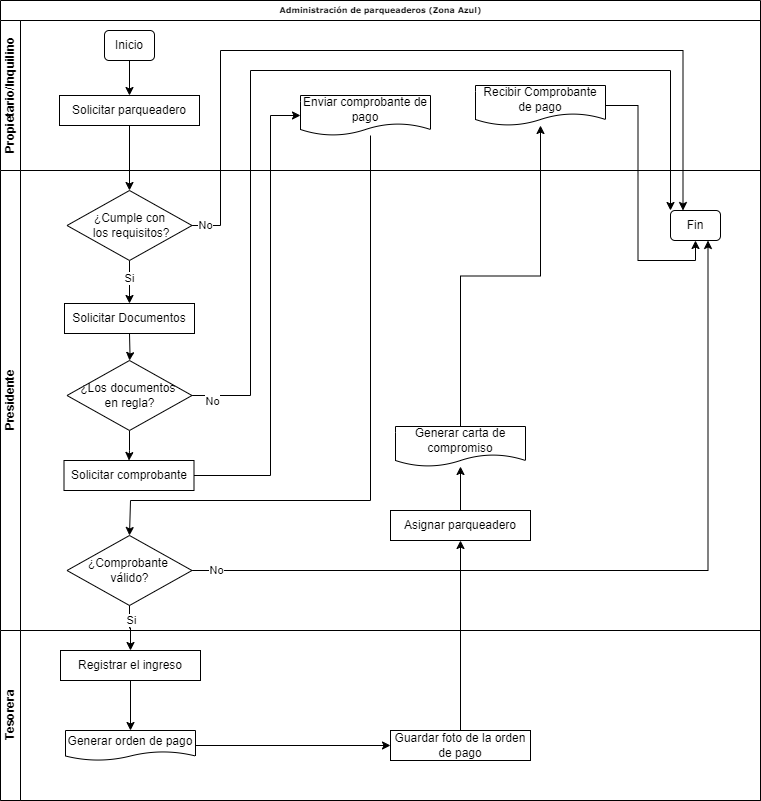
\includegraphics[width=1\textwidth]{resources/images/Diagramade flujo parqueadero-actual}
        \caption{Diagrama de flujo de procesos sistematizado prupuesto de administración de parqueaderos (Zona azul).}
        \label{fig:flujo-proceso propuesto parqueadero azul}
    \end{figure}
    \item Proceso de administración de convocatorias.
    \begin{enumerate}
        \item La directiva del conjunto se reúne para definir la fecha de la convocatoria.
        \item Se registra en el sistema la convocatoria y se notifica a los propietarios o inquilinos mediante la aplicación móvil.
        \item Se lleva a cabo la convocatoria.
        \begin{itemize}
            \item Si es una asamblea se procede al siguiente proceso.
            \item Si es una reunión o sesión de directiva se salta al proceso 6.
        \end{itemize}
        \item Los inquilinos o propietarios registran su asistencia en la aplicación móvil.
        \begin{enumerate}
            \item Si no esta registrado en el sistema el presidente o vicepresidente registra su asistencia de su domicilio al que representa.
            \item Si esta registrado en el sistema se procede al siguiente proceso.
        \end{enumerate}
        \item Se verifica la ubicación del propietario o inquilino mediante la geolocalización.
        \begin{itemize}
            \item Si se encuentra en el rango de geolocalización se registra la asistencia y se procede al siguiente proceso.
            \item Si no se encuentra en el rango de geolocalización no se registra la asistencia.
        \end{itemize}
        \item Se tratan los temas de la convocatoria.
        \item Se propone una votación de los temas a tratar.
        \begin{itemize}
            \item Si existe una votación se procede al siguiente proceso.
            \item Si no existe una votación se salta al proceso 14.
        \end{itemize}
        \item Se registra la votación en el sistema.
        \item Se habilita el voto a los propietarios o inquilinos.
        \item El sistema verifica que el usuario que va a votar sea propietario.
        \begin{itemize}
            \item Si es propietario se procede al siguiente proceso.
            \item Si no es propietario no se registra el voto.
        \end{itemize}
        \item Los propietarios registran su voto en la aplicación móvil.
        \item Se verifica la ubicación del propietario mediante la geolocalización.
        \begin{itemize}
            \item Si se encuentra en el rango de geolocalización se registra el voto y se procede al siguiente proceso.
            \item Si no se encuentra en el rango de geolocalización no se registra el voto.
        \end{itemize}
        \item Se muestra el resultado de la votación desde el sistema.
        \item Se finaliza la convocatoria.
        \item Se sube el acta de la convocatoria al sistema.
        \begin{itemize}
            \item Si es una asamblea se procede al siguiente proceso.
            \item Si es una reunión o sesión de directiva se finaliza el proceso.
        \end{itemize}
        \item Se genera el informe de inasistencia de los propietarios o inquilinos desde el sistema.
        \item Se envía el informe de asistencia a los residentes y se registra la respectiva multa en el sistema.
        \item El propietario o inquilino puede presentar una justificación por la inasistencia en las siguientes 24 horas.
        \item Se verifica la justificación presentada.
        \begin{itemize}
            \item Si la justificación es válida se procede a eliminar la multa del sistema y se finaliza el proceso.
            \item Si la justificación no es válida la multa se mantiene y termina el proceso.
        \end{itemize}
    \end{enumerate}
    \begin{figure}[H]
        \centering
        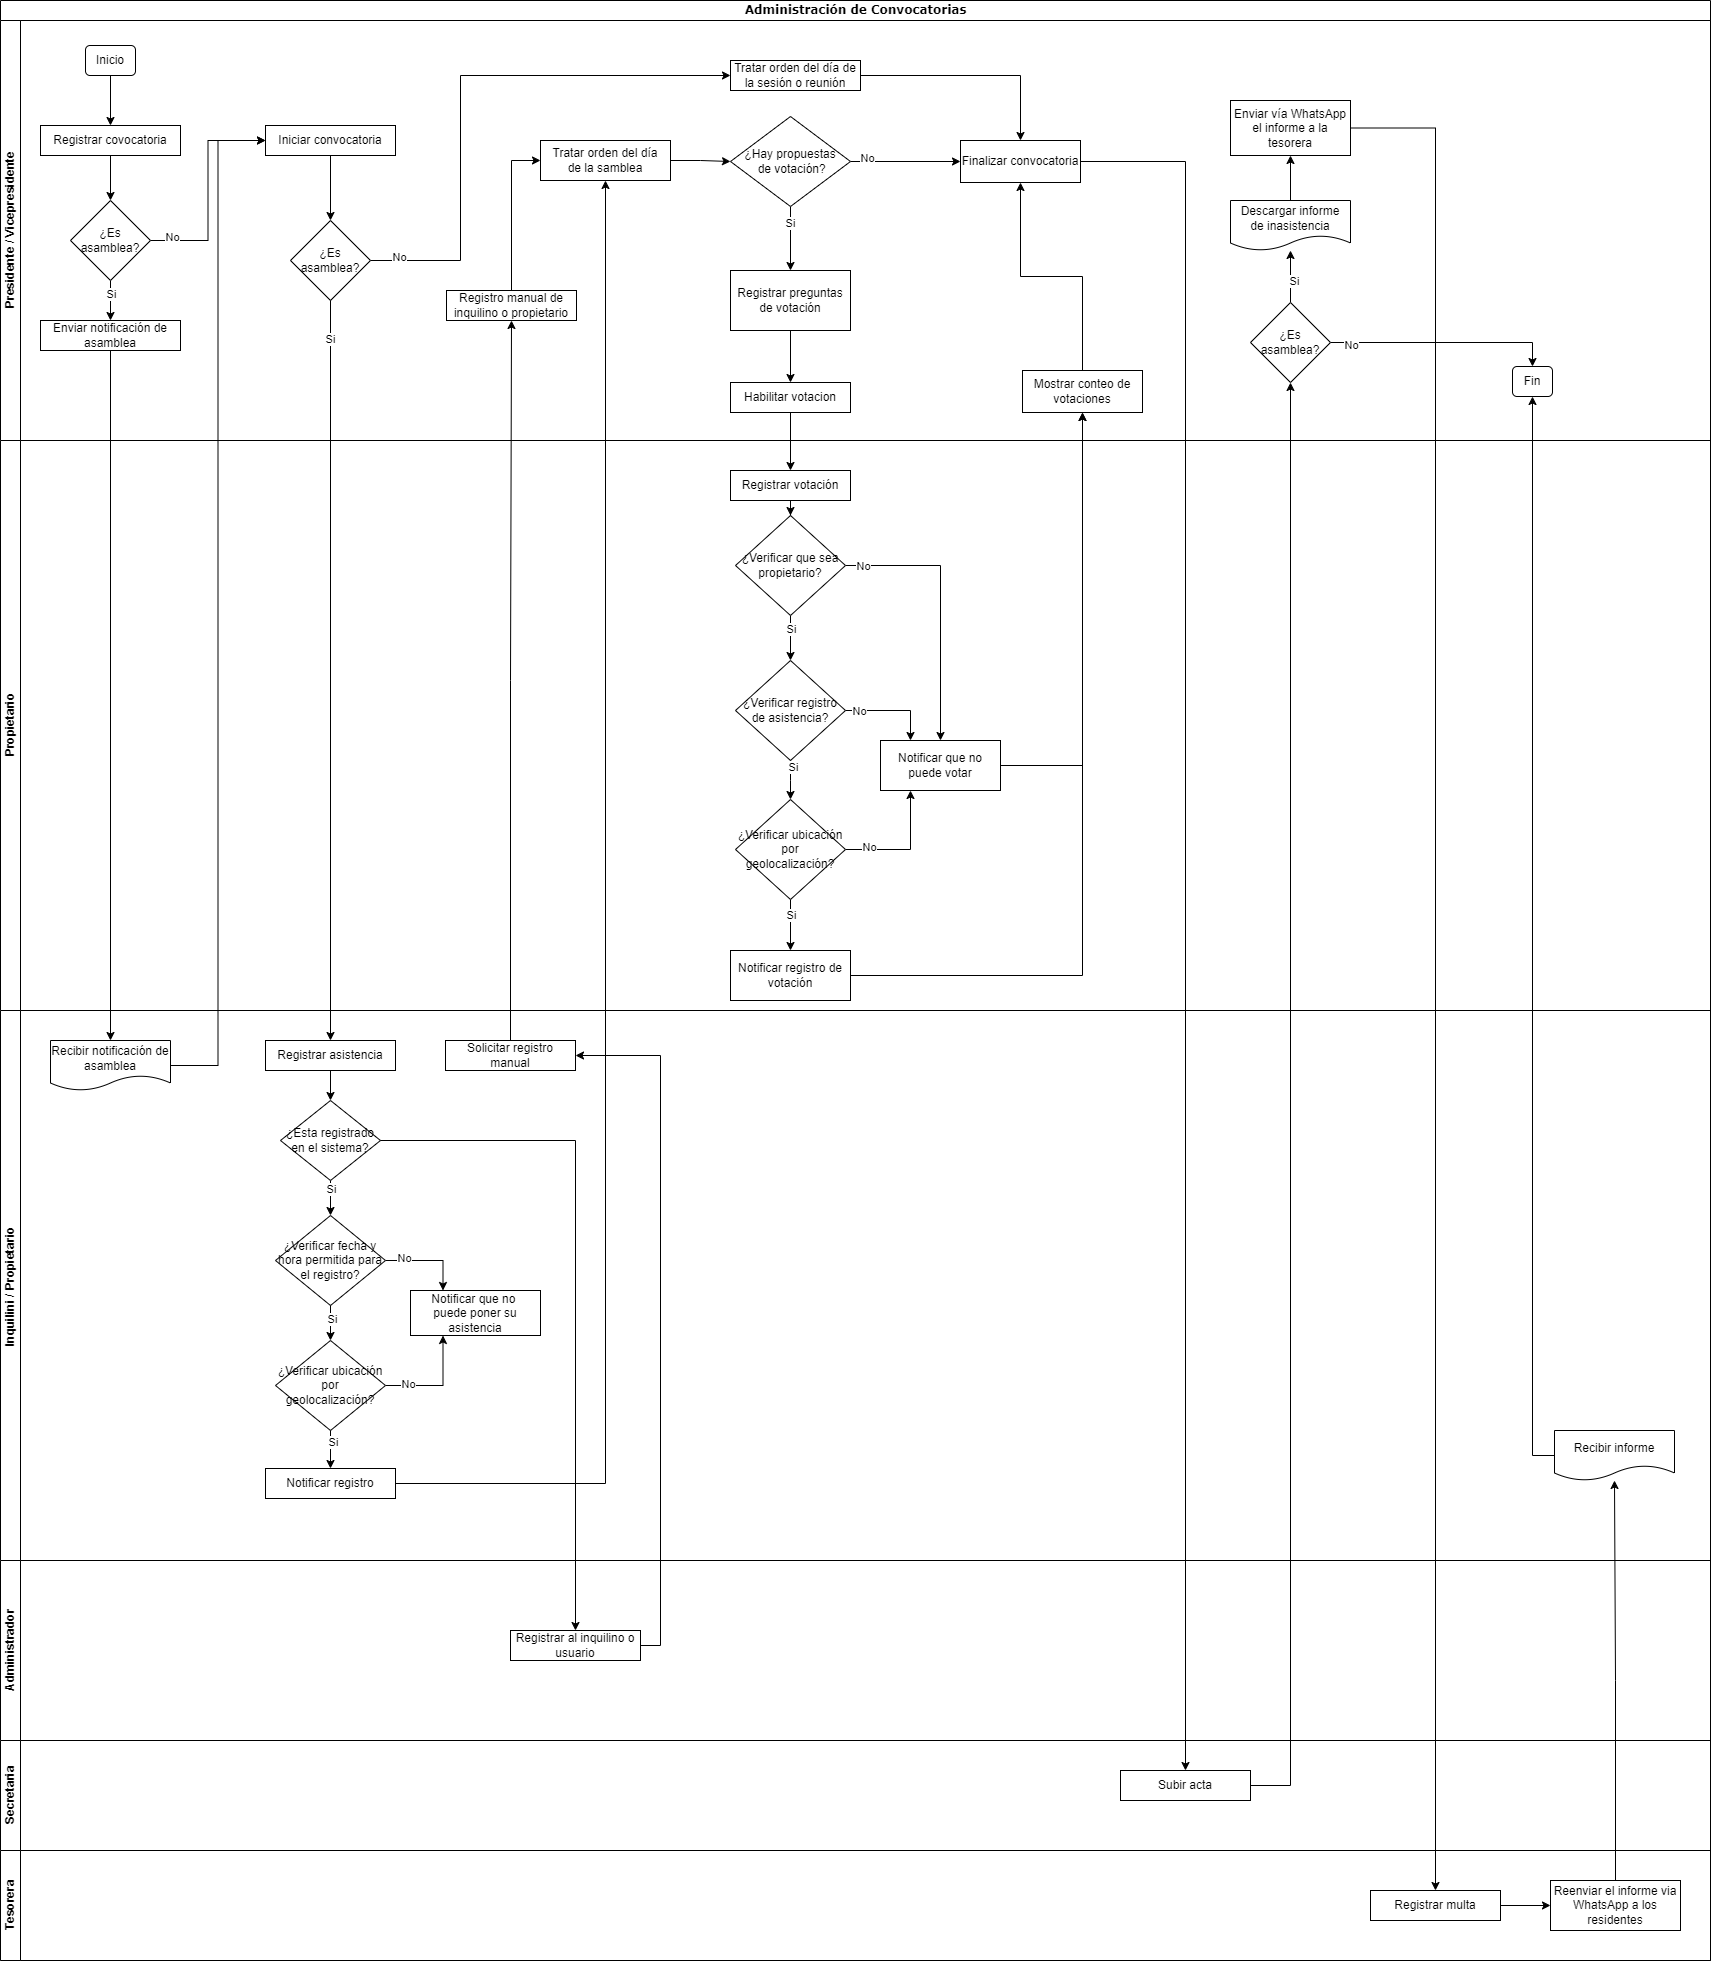
\includegraphics[width=1\textwidth]{resources/images/Diagrama de flujo convocatorias propuesto}
        \caption{Diagrama de flujo de procesos sistematizado prupuesto de convocatorias}
        \label{fig:flujo-proceso de convocatorias propuesto}
    \end{figure}


    \item Proceso de administración financiera.
    \begin{enumerate}
        \item Pagos de obligaciones financieras mensuales
        \begin{enumerate}
            \item El inquilino realiza el pago de la mensualidad de sus obligaciones financieras.
            \item El inquilino envía el comprobante de pago a la tesorera.
            \item La tesorera verifica el comprobante de pago.
            \begin{itemize}
                \item Si el comprobante es válido se procede al siguiente proceso.
                \item Si el comprobante no es válido se notifíca via WhatsApp y se finaliza el proceso.
            \end{itemize}
            \item La tesorera selecciona la residencia del inquilino o propietario.
            \item El sistema verifica hasta que mes abonó el inquilino en su anterior pago.
            \begin{itemize}
                \item Si el inquilino tiene abonos anteriores el sistema coloca el mes siguiente de manera automática y se procede al siguiente paso.
                \item Si el inquilino no tiene abonos se procede al siguiente paso.
            \end{itemize}
            \item Se registra el pago en el sistema.
            \item Se sube el comprobante de pago al sistema.
            \item Se genera una orden de pago.
            \item Se envía por correo electrónico el respaldo de pago al inquilino o propietario.
        \end{enumerate}
        \begin{figure}[H]
            \centering
            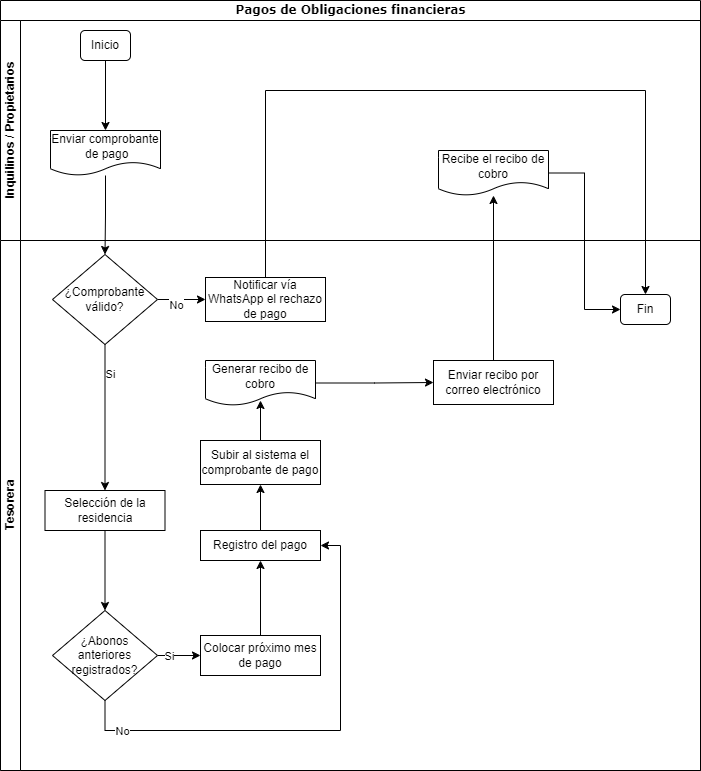
\includegraphics[width=1\textwidth]{resources/images/Diagrama de flujo de proceso pagos obligaciones propuesto}
            \caption{Diagrama de flujo de procesos sistematizado prupuesto de pago de obligaciones financieras mensuales}
            \label{fig:flujo-proceso-pago de obligaciones financieras propuesto}
        \end{figure}

        \item Pagos a proveedores
        \begin{enumerate}
            \item El proveedor envía la factura a la tesorera.
            \item La tesorera verifica la factura.
            \begin{itemize}
                \item Si la factura es válida se procede al siguiente proceso.
                \item Si la factura no es válida se finaliza el proceso.
            \end{itemize}
            \item La tesorera verifíca si el proveedor está registrado en el sistema.
            \begin{itemize}
                \item Si el proveedor está registrado se procede al siguiente proceso.
                \item Si el proveedor no está registrado se le registra en el sistema y se repite el proceso.
            \end{itemize}
            \item La tesorera registra la factura en el sistema.
            \item Se sube la factura al sistema.
        \end{enumerate}

        \begin{figure}[H]
            \centering
            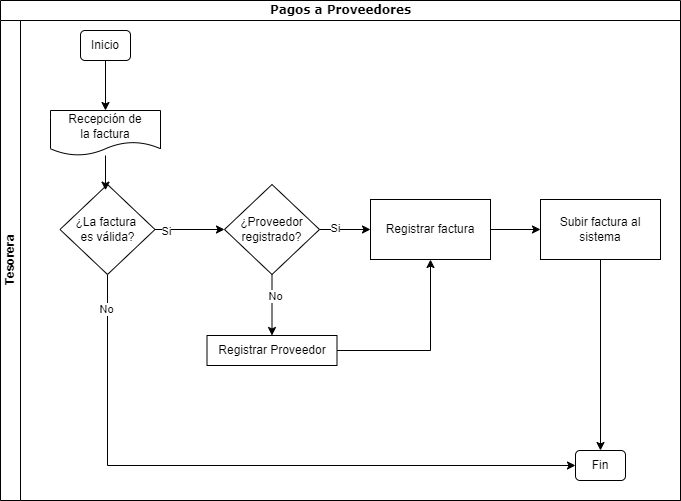
\includegraphics[width=1\textwidth]{resources/images/Diagrama de flujo de proceso pagos a proveedores propuesto}
            \caption{Diagrama de flujo de procesos sistematizado prupuesto de pago a proveedores}
            \label{fig:flujo-proceso-ppago proveedores propuesto}
        \end{figure}
        \item Multas
        \begin{enumerate}
            \item Se registra la multa en el sistema.
            \item Se suben evidencias de la multa al sistema.
            \item Se le notifica al propietario o inquilino la multa mediante la aplicación móvil.
            \item El propietario o inquilino envía el comprobante de pago de la multa.
            \item La tesorera verifica el comprobante de pago.
            \begin{itemize}
                \item Si el comprobante es válido se procede al siguiente proceso.
                \item Si el comprobante no es válido se mantiene la multa, se le notifica por la aplicación móvil el rechazo del pago y se finaliza el proceso.
            \end{itemize}
            \item Se actualiza el estado de la multa en el sistema.
            \item Se genera una orden de pago.
            \item El sistema envía por correo electrónico el respaldo de pago al propietario o inquilino.
        \end{enumerate}
        \begin{figure}[H]
            \centering
            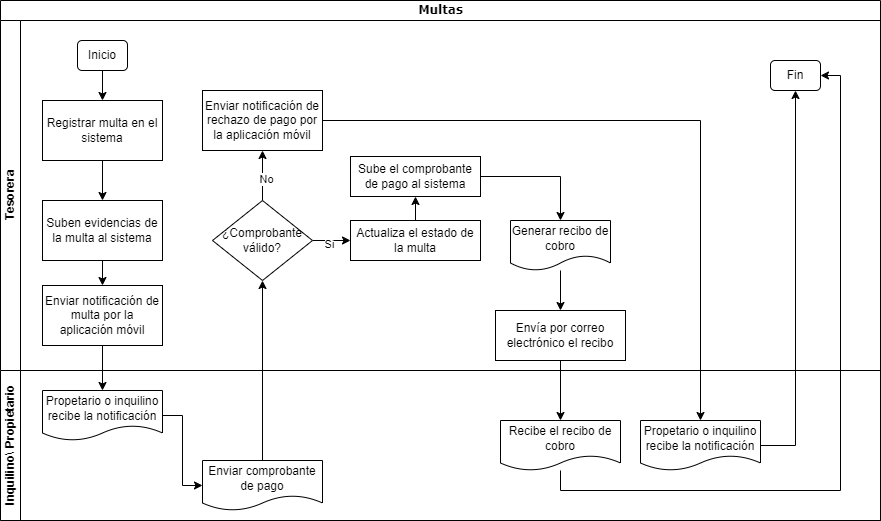
\includegraphics[width=1\textwidth]{resources/images/Diagrama de flujo de proceso multas propuesta}
            \caption{Diagrama de flujo de procesos sistematizado prupuesto de multas}
            \label{fig:flujo-proceso-prupuesto-multas}
        \end{figure}
    \end{enumerate}
\end{itemize}


\subsubsection{Arquitectura}

Para el desarrollo de la propuesta se utilizó una arquitectura cliente-servidor.
El cliente permite a los usuarios interactuar con el sistema mediante la aplicación móvil y el sistema web.
En donde las personas que son parte de la directiva tendrán acceso al sistema web y los propietarios o inquilinos accederán únicamente a la aplicación móvil.
Por otro lado la API que estará alojada en el servidor se encargara de procesar las peticiones de los clientes provenientes de la aplicación móvil y el sistema web, en  donde se proveerán de servicios necesarios para satisfacer los requerimientos tal y como se muestra en la Figura \ref{fig:arquitectura}.
Además de ofrecernos la conexión a la base de datos para la persistencia de los datos.
La base de datos la cual también se encontrará alojada en el servidor, nos permitirá almacenar y servir la información necesaria para el funcionamiento del sistema.
Por último la API se conectará a los servicios de almacenamiento de archivos de AWS S3 para la carga de archivos necesarios para el sistema.

\begin{figure}[H]
    \centering
    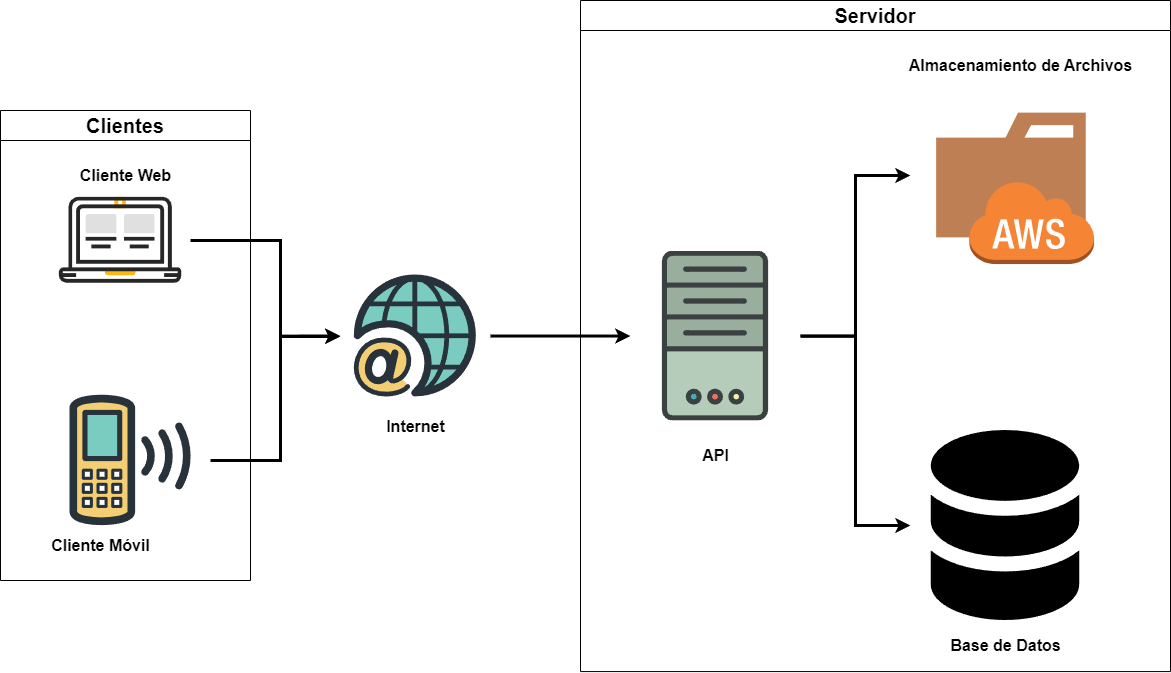
\includegraphics[width=1\textwidth]{resources/images/Arquitectura}
    \caption{Arquitectura del sistema}
    \label{fig:arquitectura}
\end{figure}

\subsubsection{Prototipado}

Con la finalidad de poder presentar a los usuarios finales una vista previa de cómo se verán los sistemas y también como parte de la fase de la metodología RAD se realizaron prototipos de las interfaces de usuario del sistema web y la aplicación móvil.
\bigbreak

\textbf{Prototipo web}
\bigbreak
En la Figura \ref{fig:login} se muestra la vista de la pantalla de inicio de sesión web de los usuarios miembros de la directiva en donde el usuario podrá ingresar sus credenciales para acceder al sistema y en el caso de ser necesario recuperar su contraseña a través de su correo electrónico.

\begin{figure}[H]
    \centering
    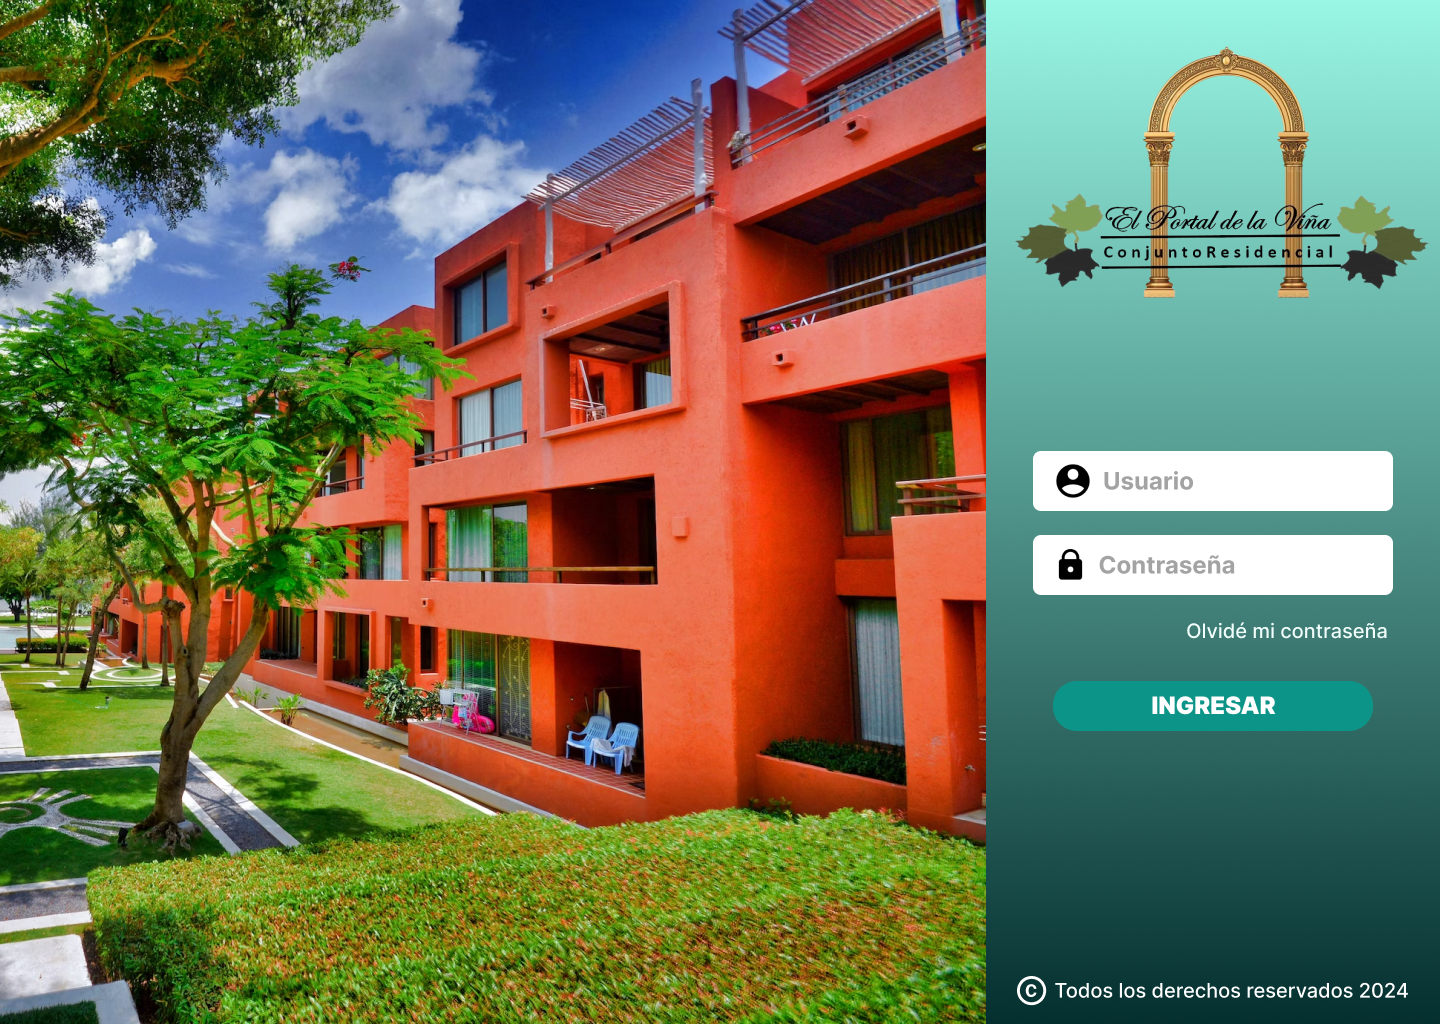
\includegraphics[width=1\textwidth]{resources/images/login}
    \caption{Prototipo de inicio de sesión}
    \label{fig:login}
\end{figure}

En la Figura \ref{fig:nevagacion} se muestra la vista de la barra de navegación del sistema web en donde se visualizan las opciones de menú disponibles para los usuarios miembros de la directiva y en la parte inferior de la misma se muestra el nombre del usuario que ha iniciado sesión asi como la opción de cerrar sesión.

\begin{figure}[H]
    \centering
    
\includegraphics[width=1\textwidth]{resources/images/navegacion}
    \caption{Prototipo de la vista del la barra de navegación}
    \label{fig:nevagacion}
\end{figure}


Una vez iniciada la sesión se mostrara una vista de dashboard en donde se visualizará información relevante para los usuarios miembros de la directiva dependiendo de quien haya iniciado sesión, en el caso de la Figura \ref{fig:dashboard} se muestra la vista del dashboard para el administrador, en la Figura \ref{fig:dashboard-presidente} se muestra la vista del dashboard para presidente y vicepresidente y por último en la Figura \ref{fig:dashboard-tesorera} se muestra la vista del dashboard para la tesorera.

\begin{figure}[H]
    \centering
    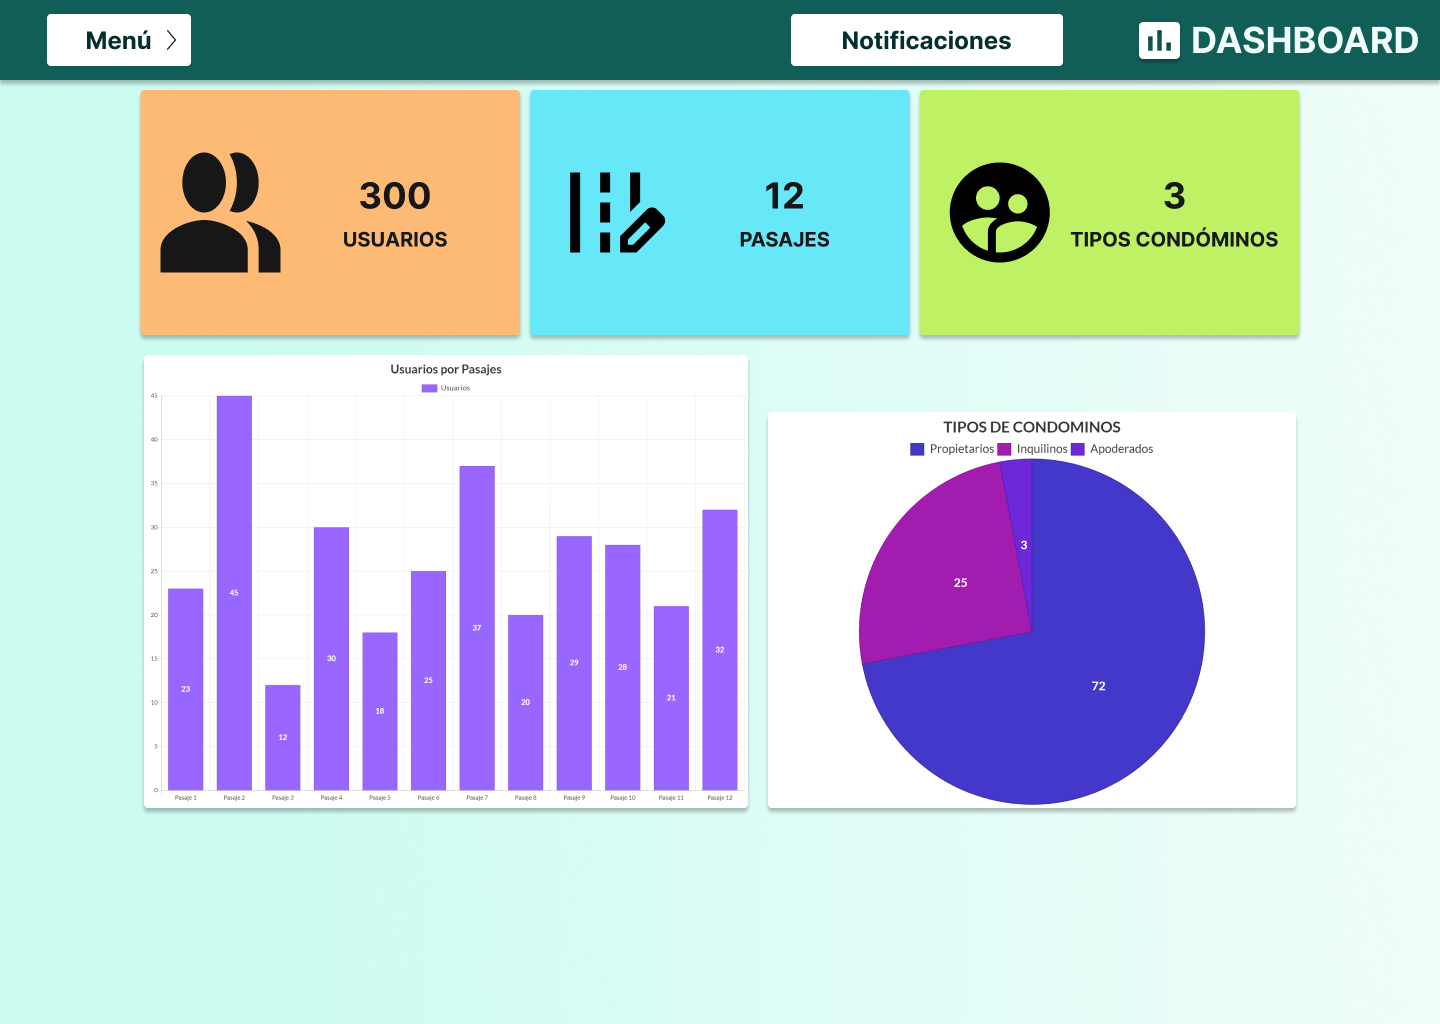
\includegraphics[width=1\textwidth]{resources/images/dashboard}
    \caption{Prototipo de la vista del dashboard de administración}
    \label{fig:dashboard}
\end{figure}

\begin{figure}[H]
    \centering
    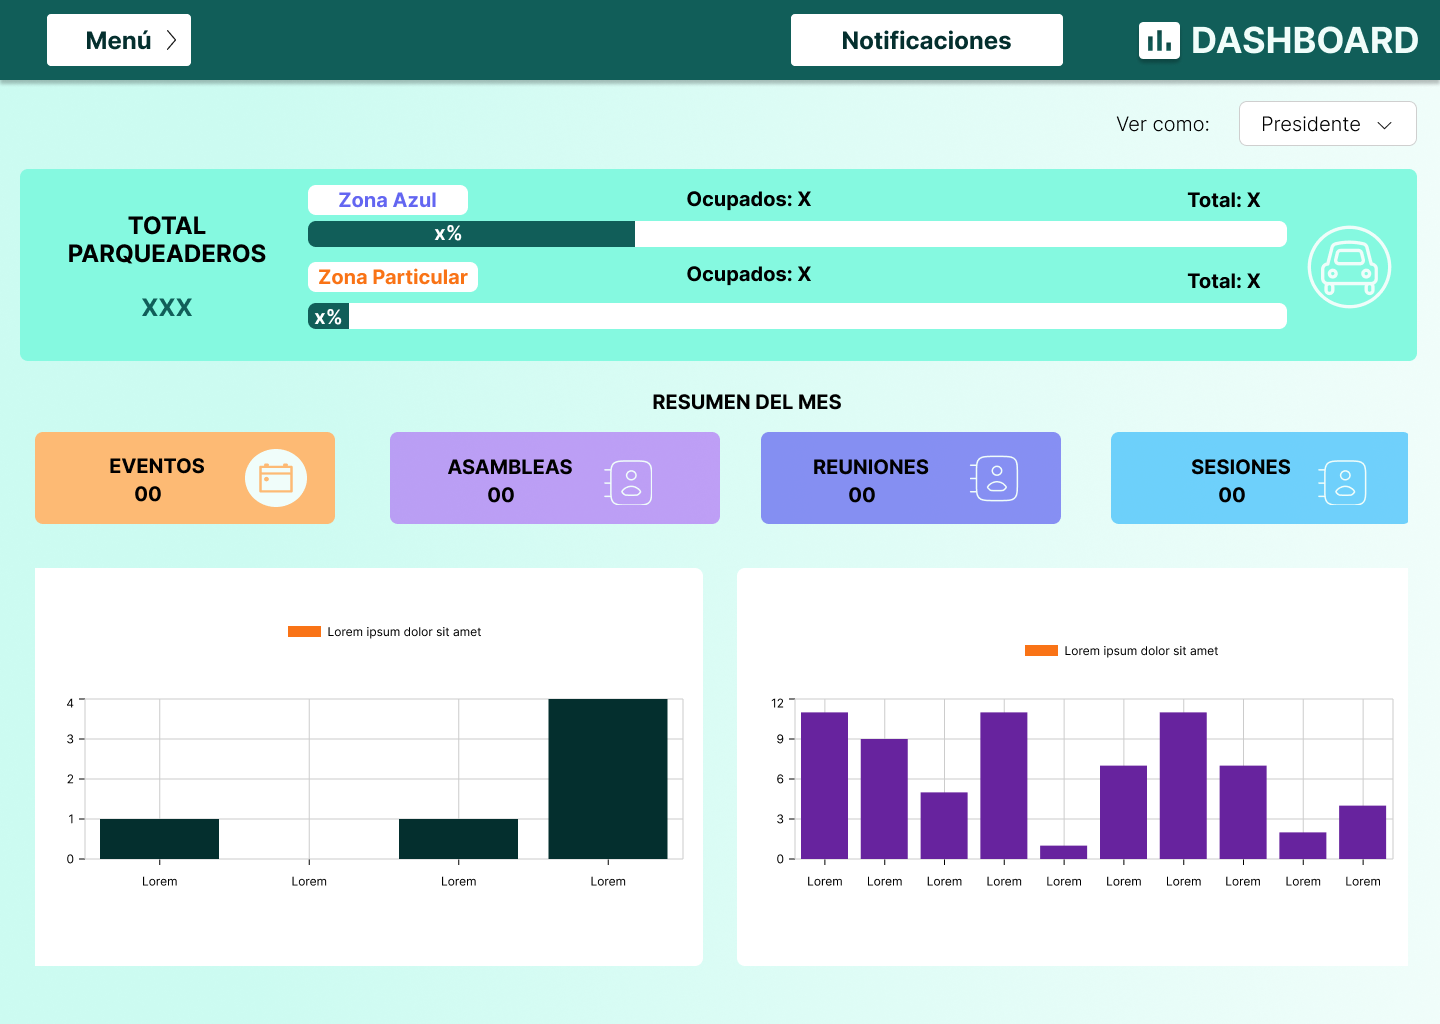
\includegraphics[width=1\textwidth]{resources/images/Dashboard-view-presidente}
    \caption{Prototipo de la vista del dashboard de presidencia}
    \label{fig:dashboard-presidente}
\end{figure}

\begin{figure}[H]
    \centering
    \includegraphics[width=1\textwidth]{resources/images/Dashboard-view-tesorería}
    \caption{Prototipo de la vista del dashboard de tesorería}
    \label{fig:dashboard-tesorera}
\end{figure}

En la Figura \ref{fig:usuarios} se muestra la vista de la administración de usuarios en donde el administrador podrá visualizar, registrar, inhabilitar o editar la información y roles de los demás usuarios.

\begin{figure}[H]
    \centering
    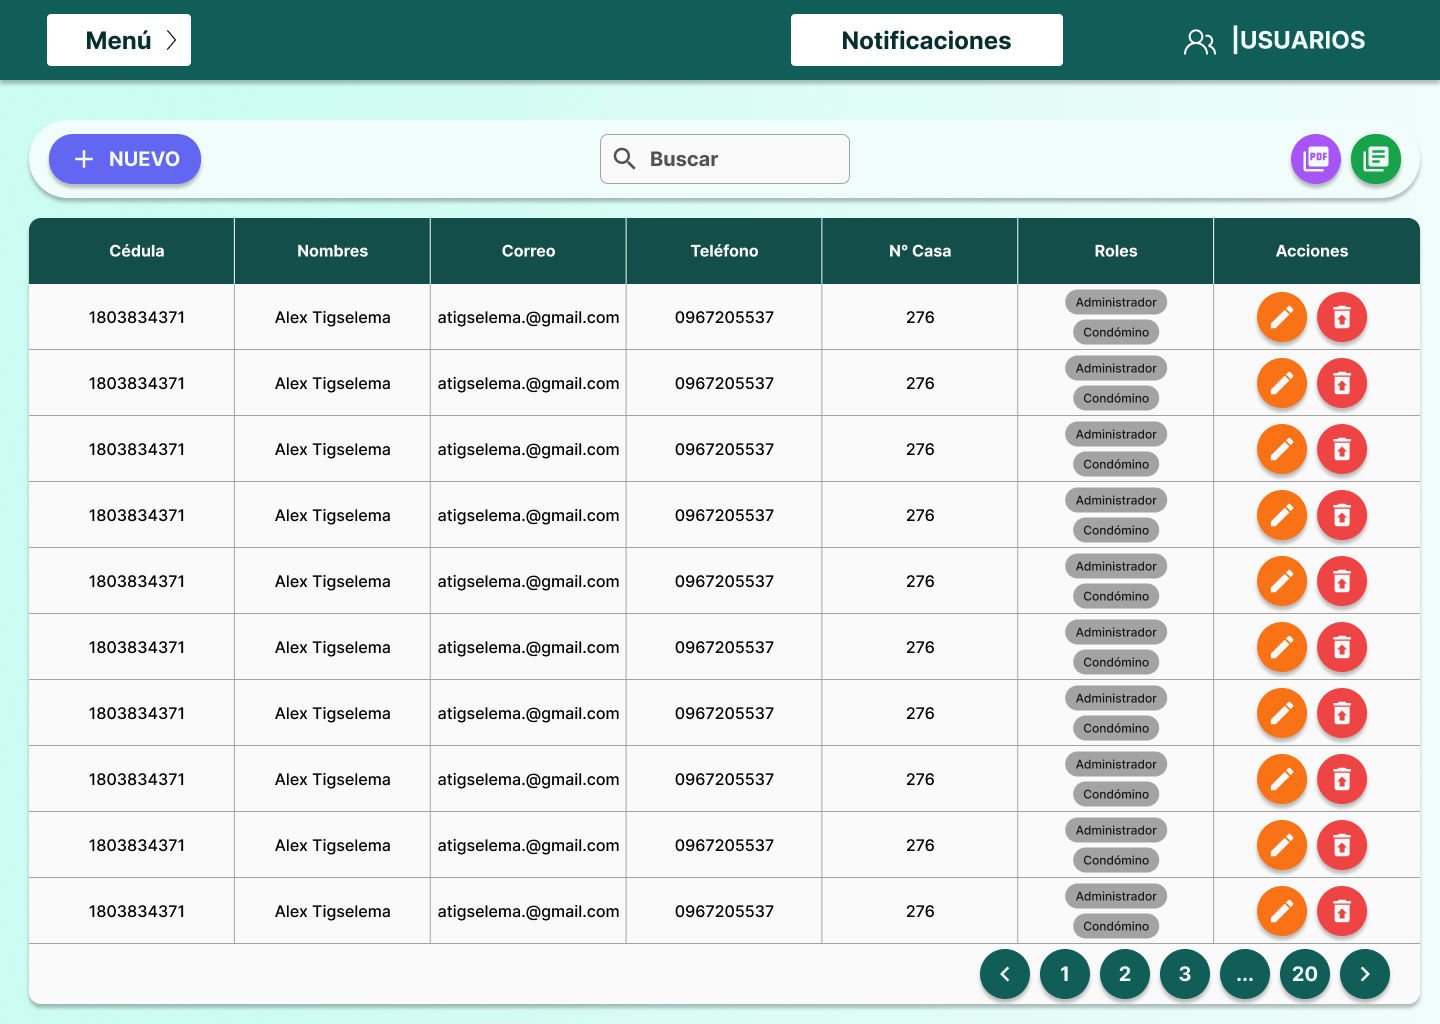
\includegraphics[width=1\textwidth]{resources/images/usuarios}
    \caption{Prototipo de la vista de la administración de usuarios}
    \label{fig:usuarios}
\end{figure}

En la Figura \ref{fig:usuarios formulario} se muestra la vista del formulario para edición o creación de usuarios, en donde el administrador podrá ingresar la información necesaría y seleccionar el rol que cumplirá el usuario a ingresar o editar.

\begin{figure}[H]
    \centering
    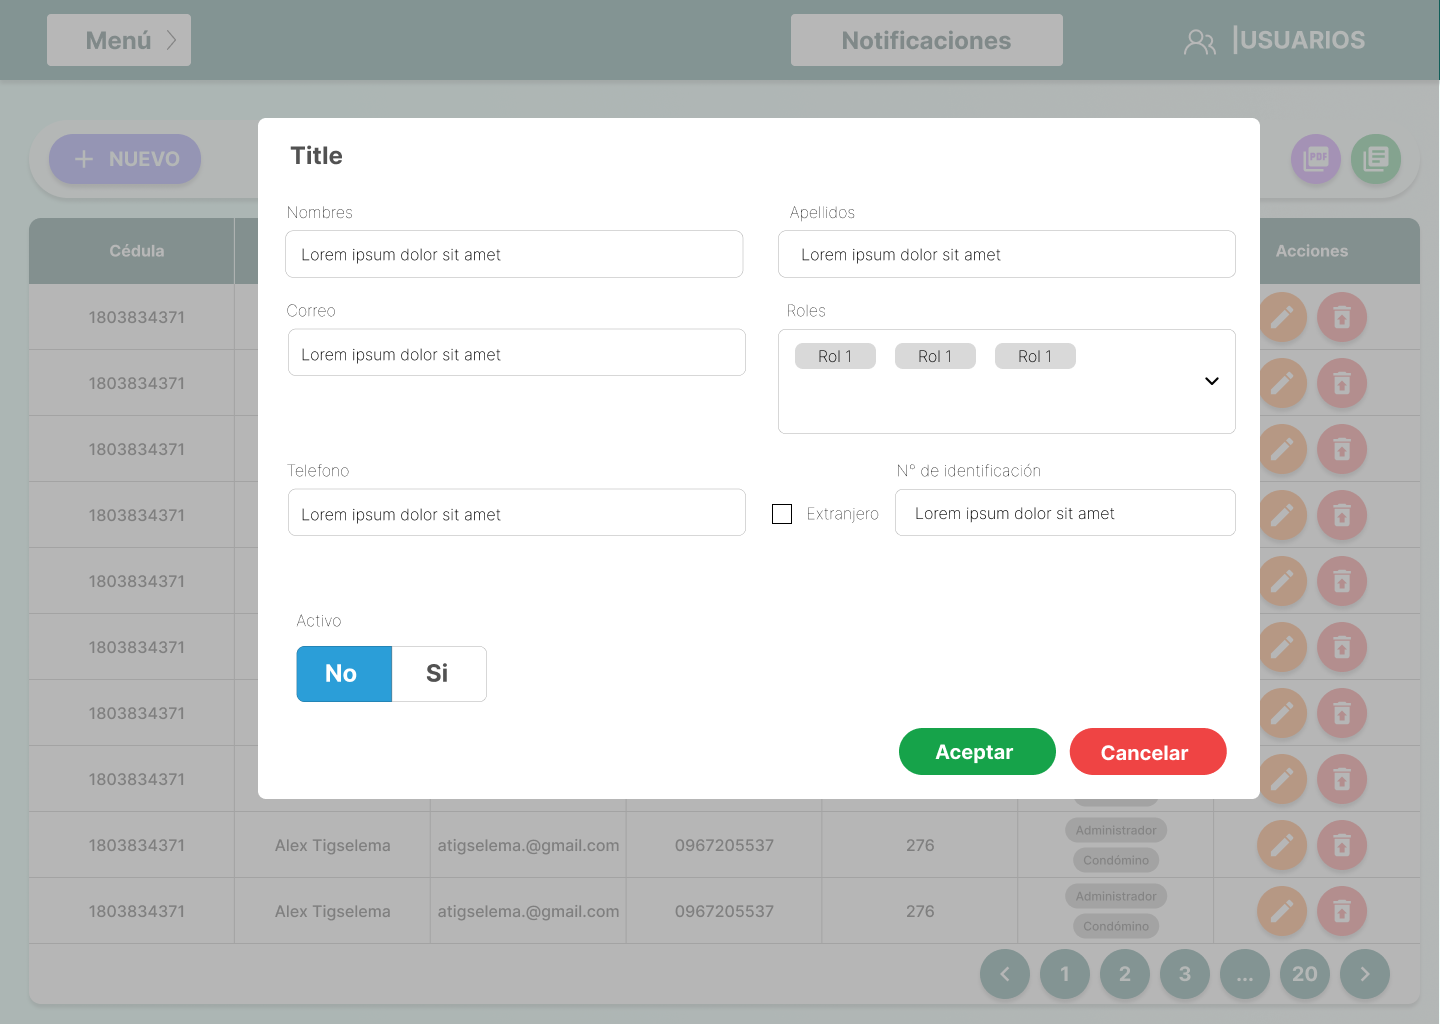
\includegraphics[width=1\textwidth]{resources/images/usuarios formulario}
    \caption{Prototipo de la vista del fomulario para edición o creación de usuarios}
    \label{fig:usuarios formulario}
\end{figure}

En la Figura \ref{fig:geolocalizacion} se muestra la vista de la configuración de la geolocalización en donde el administrador podrá editar la ubicación de las coordenadas y el radio de aceptación mediante la visualización de un mapa del lugar en donde se darán lugar las asambleas.

\begin{figure}[H]
    \centering
    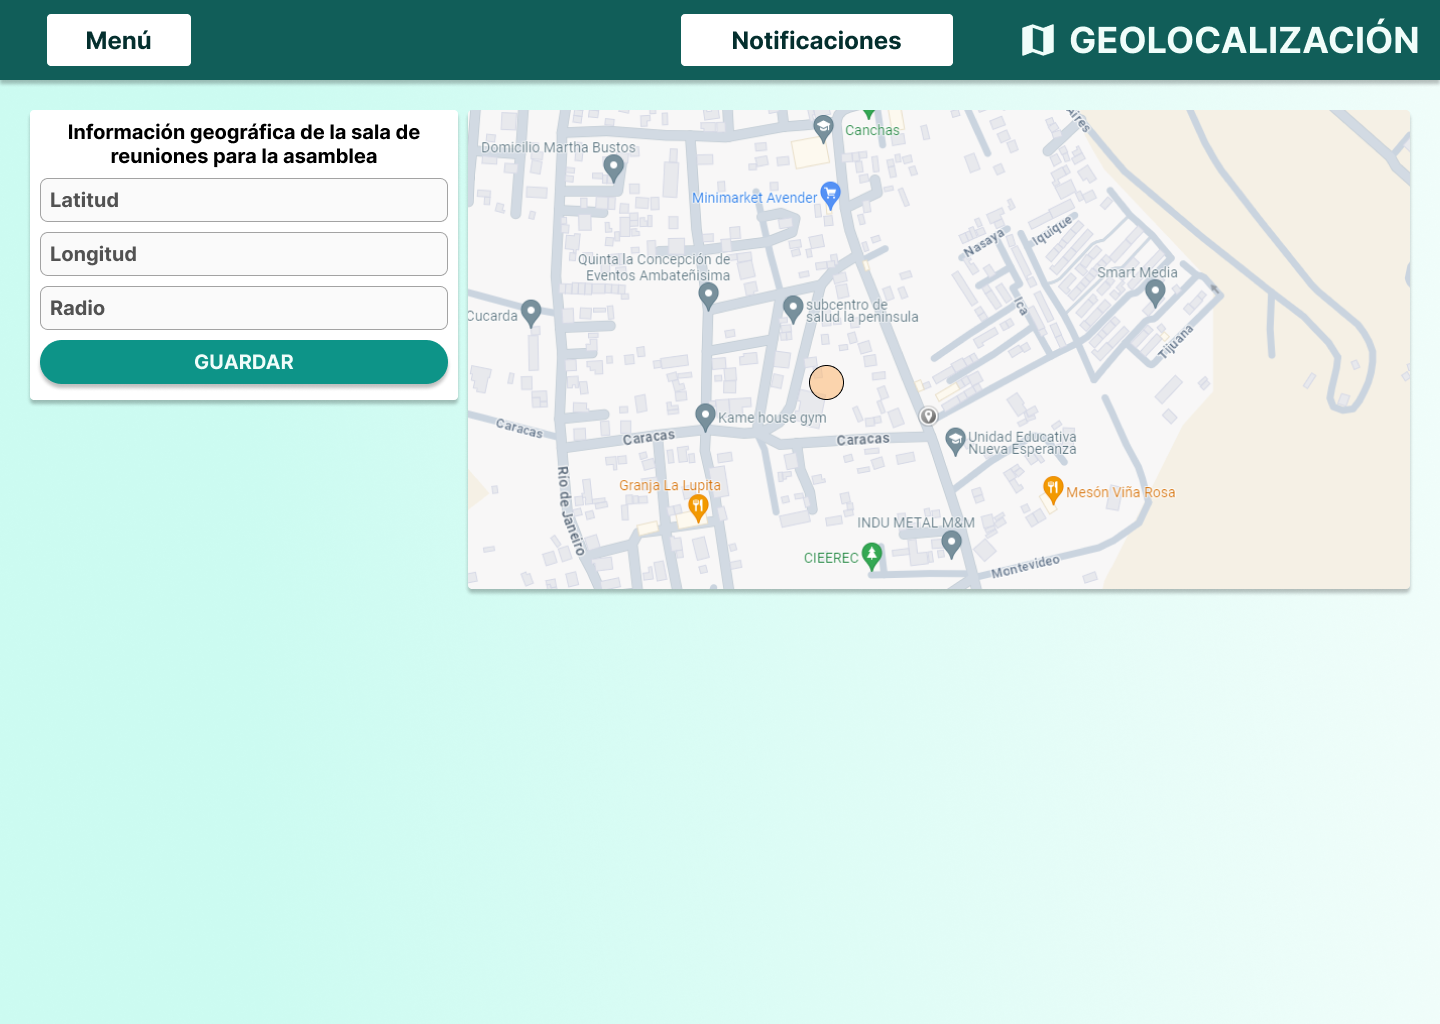
\includegraphics[width=1\textwidth]{resources/images/geolocalizacion}
    \caption{Prototipo de la vista de la configuración de la geolocalización}
    \label{fig:geolocalizacion}
\end{figure}

En la Figura \ref{fig:residencias} se muestra la vista de la administración de residencias en donde el presidente o vicepresidente podrán visualizar o desplegar el formulario de actualización de residente de cada residencia.

\begin{figure}[H]
    \centering
    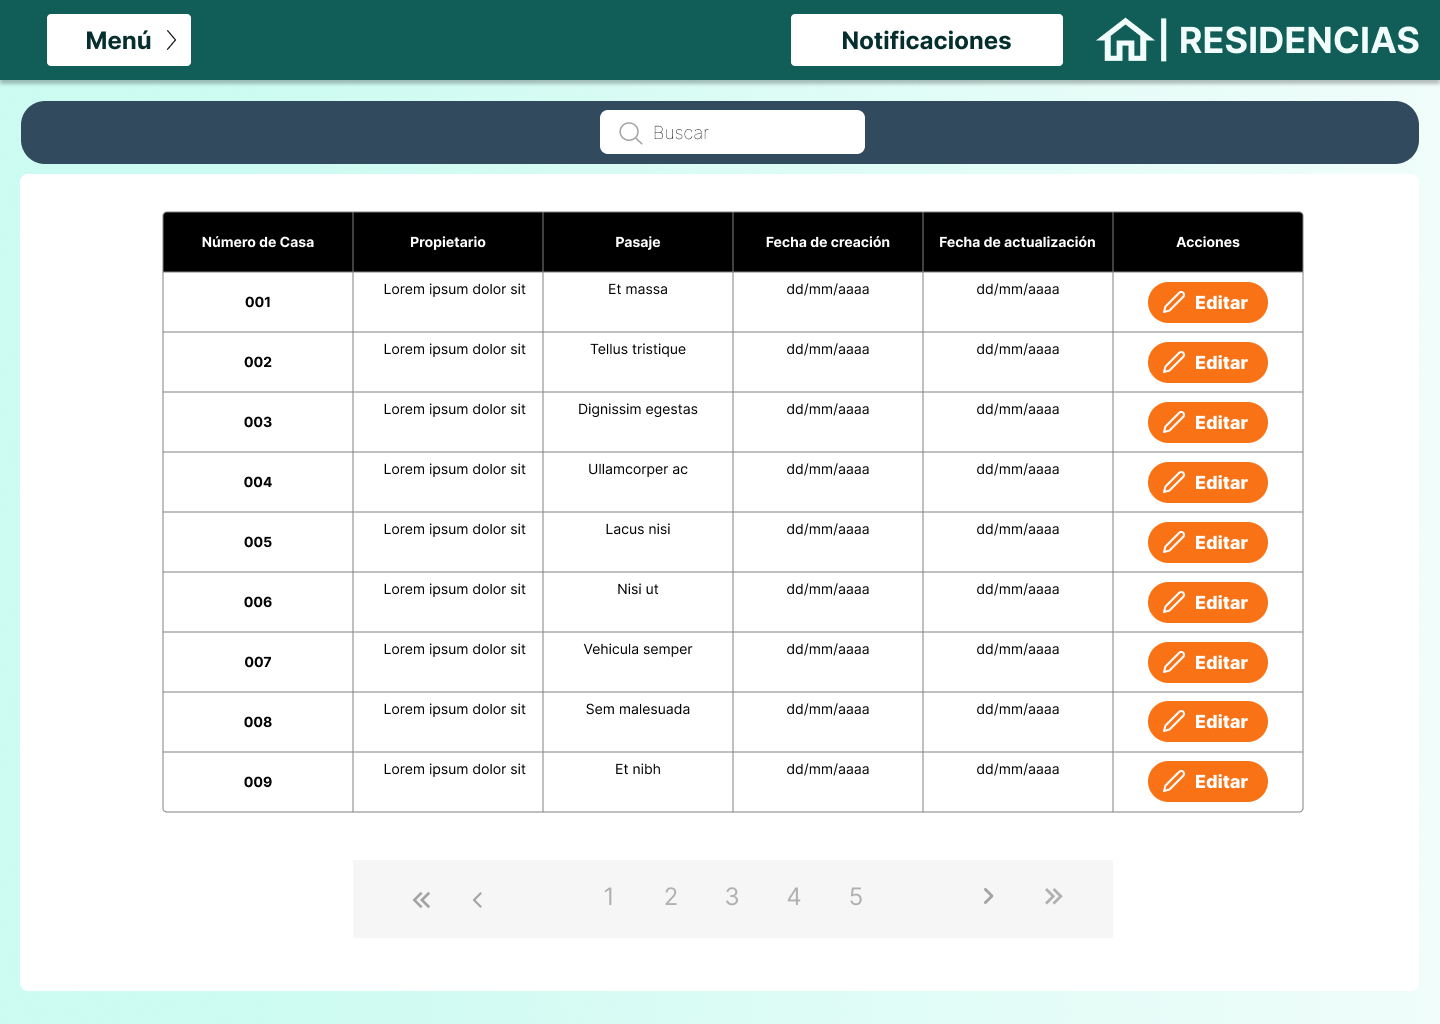
\includegraphics[width=1\textwidth]{resources/images/residencias}
    \caption{Prototipo de la vista de administración de residencias}
    \label{fig:residencias}
\end{figure}


En la Figura \ref{fig:parqueaderos} se muestra la vista de la administración de parqueaderos, en donde mediante la representación de un mapa del condominio el presidente puede visualizar los grupos de parqueaderos por colores en donde los amarillos representan a los parqueaderos partículares y los azules los de zona azul.
Por cada grupo se desplegara una vista emergente de los parqueaderos que forman parte de ese grupo junto con su código de numeración y su estado,
en donde el presidente podrá seleccionar un parqueadero y desplegar el formulario de cambio de residencia asociada a ese parqueadero.
En la parte superior se muestra una barra de navegación para poder cambiar a la vista de visualización de los tipos de parqueaderos Figura \ref{fig:parqueaderos tipos}.
\begin{figure}[H]
    \centering
    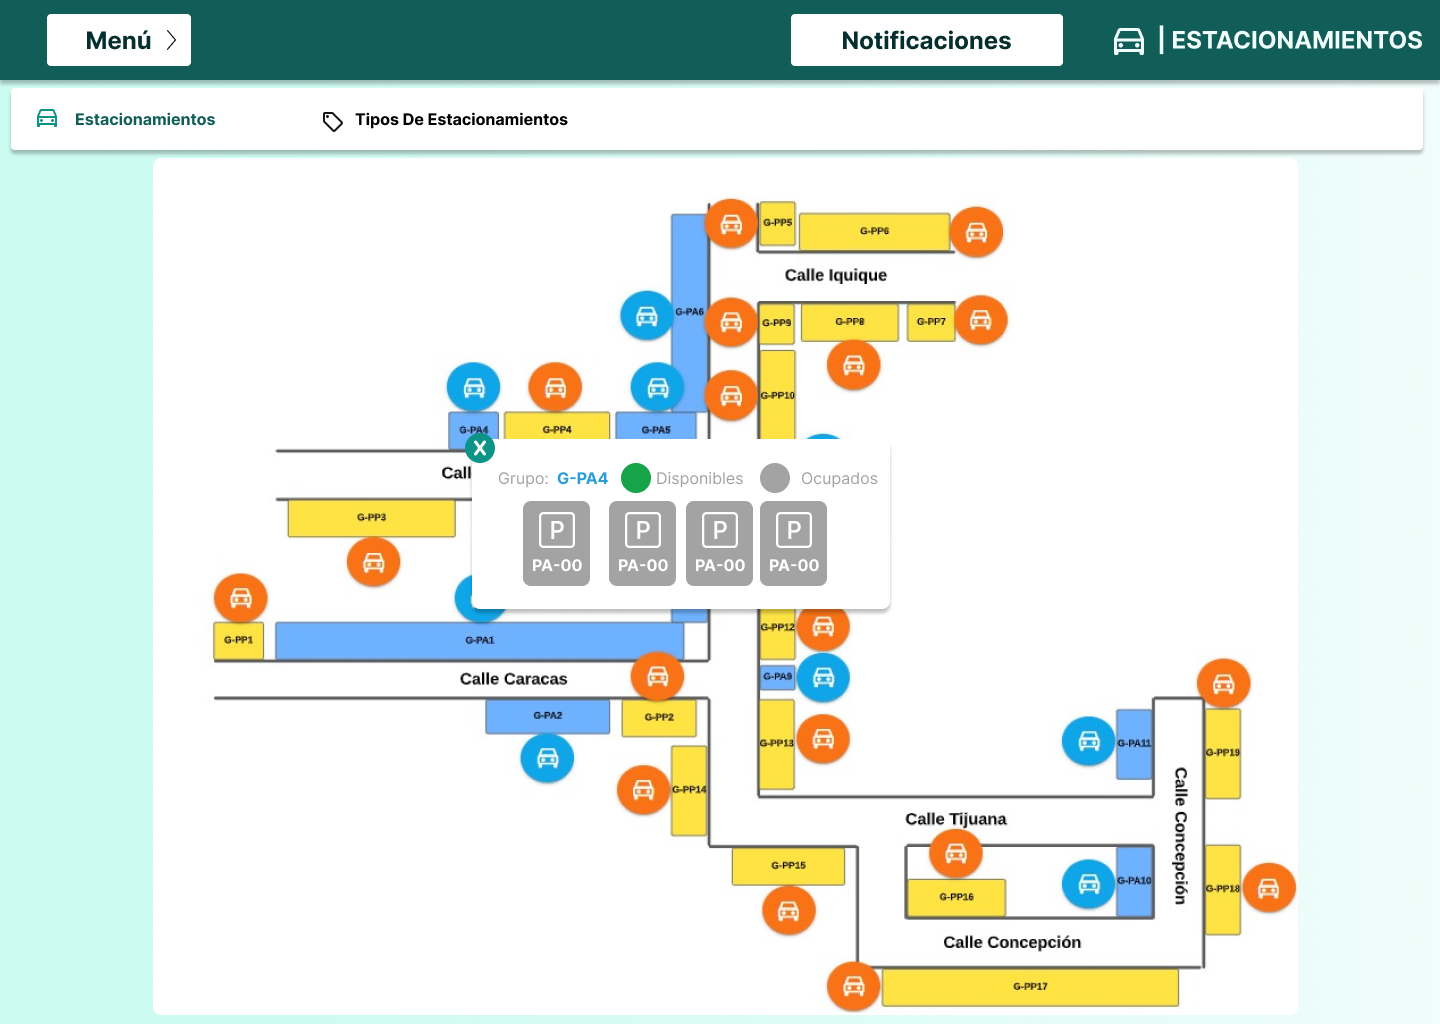
\includegraphics[width=1\textwidth]{resources/images/estacionamientos-organization}
    \caption{Prototipo de la vista de administración de parqueaderos}
    \label{fig:parqueaderos}
\end{figure}

\begin{figure}[H]
    \centering
    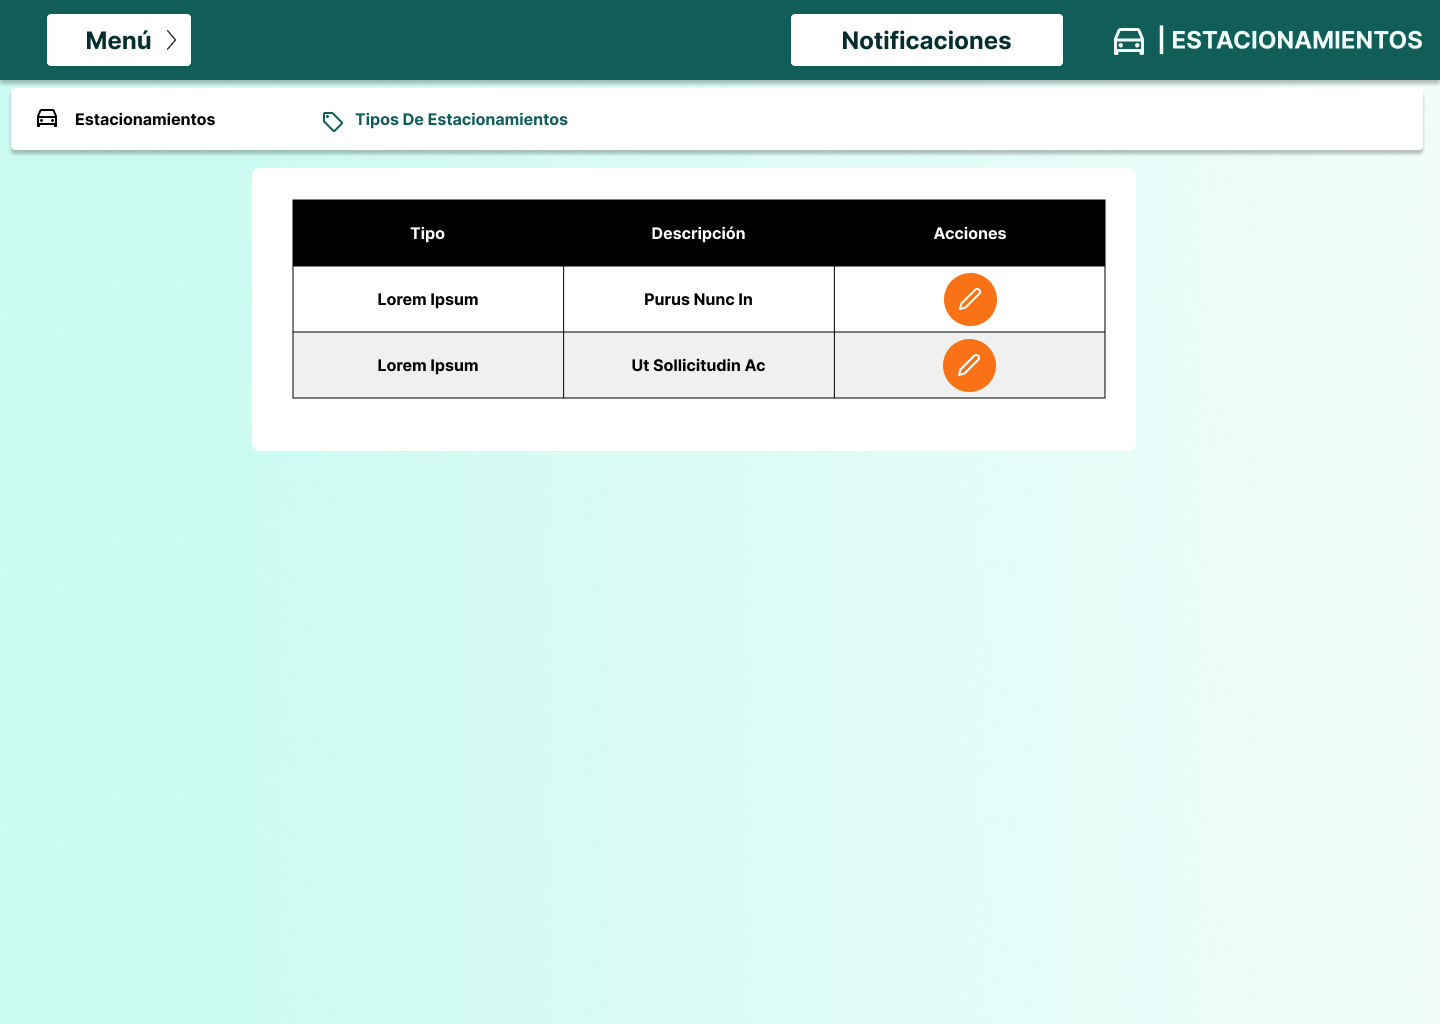
\includegraphics[width=1\textwidth]{resources/images/estacionamientos- type}
    \caption{Prototipo de la vista de administración de tipos de parqueaderos}
    \label{fig:parqueaderos tipos}
\end{figure}

En la Figura \ref{fig:parqueaderos formulario} se muestra la vista del formulario de cambio de residencia asociada a un parqueadero, en donde el presidente podrá seleccionar un residente mediante una tabla de búsqueda Figura \ref{fig:parqueaderos formulario seleccion residente} y seleccionar la residencia que se asociará al parqueadero.

\begin{figure}[H]
    \centering
    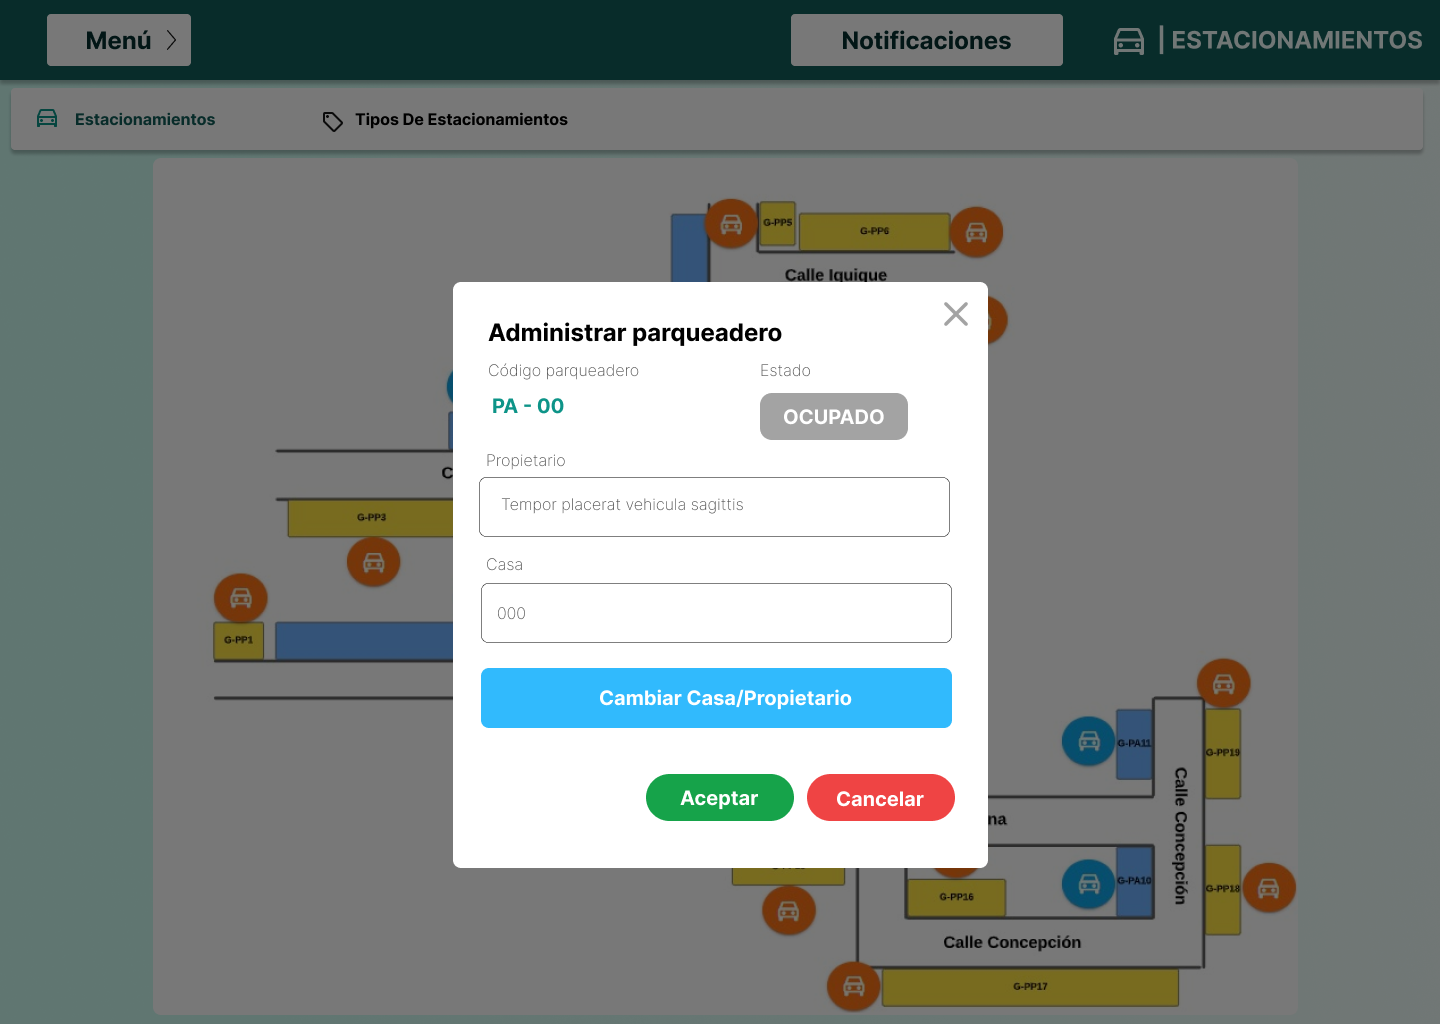
\includegraphics[width=1\textwidth]{resources/images/estacionamientos-organization-form}
    \caption{Prototipo de la vista del formulario de cambio de residencia asociada a un parqueadero}
    \label{fig:parqueaderos formulario}
\end{figure}

\begin{figure}[H]
    \centering
    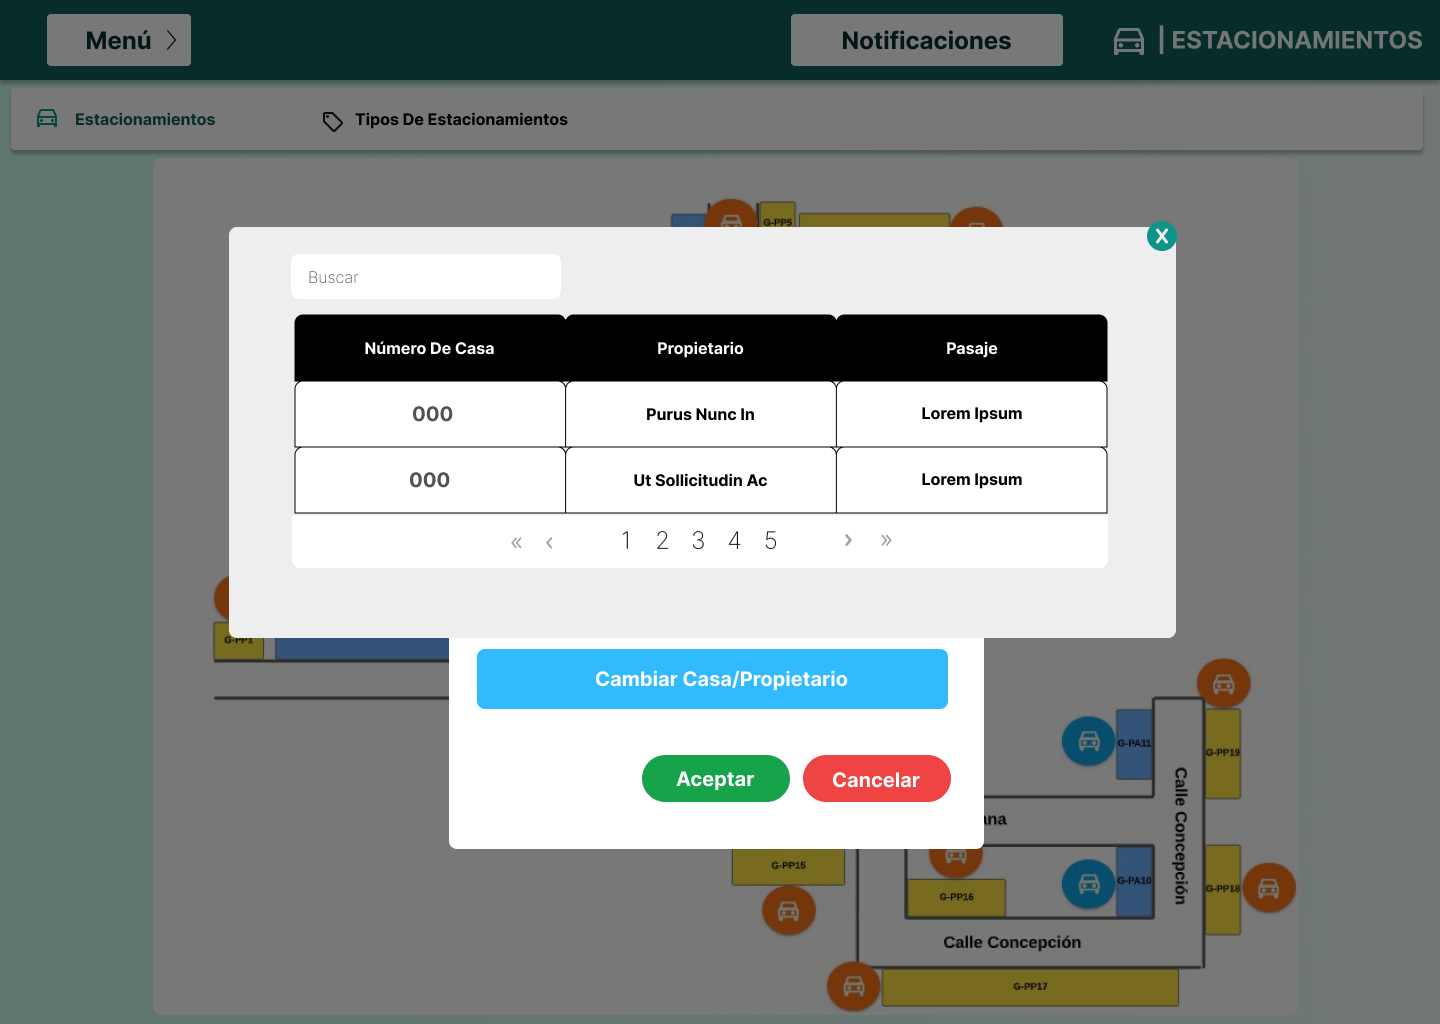
\includegraphics[width=1\textwidth]{resources/images/estacionamientos-form-vista}
    \caption{Prototipo de la vista del formulario en la selección de residencia}
    \label{fig:parqueaderos formulario seleccion residente}
\end{figure}

En la Figura \ref{fig:convocatorias} se muestra la vista de la administración de convocatorias en donde el presidente o vicepresidente podrán visualizar las convocatorias junto con la información relevante de cada una, registrar o editar una convocatoria mediante un formulario Figura \ref{fig:convocatorias-edit}, además de poder desplegar un menú de opciones en donde se podrá visualizar un pista previa de la convocatoria para ser descargada en formato PDF Figura \ref{fig:convocatorias-ver}, finalizar la convocatoria, administrar la asistencia Figura \ref{fig:convocatorias-asistentes} o administrar las votaciones en el caso de ser una asamblea Figura \ref{fig:convocatorias-votaciones}.

\begin{figure}[H]
    \centering
    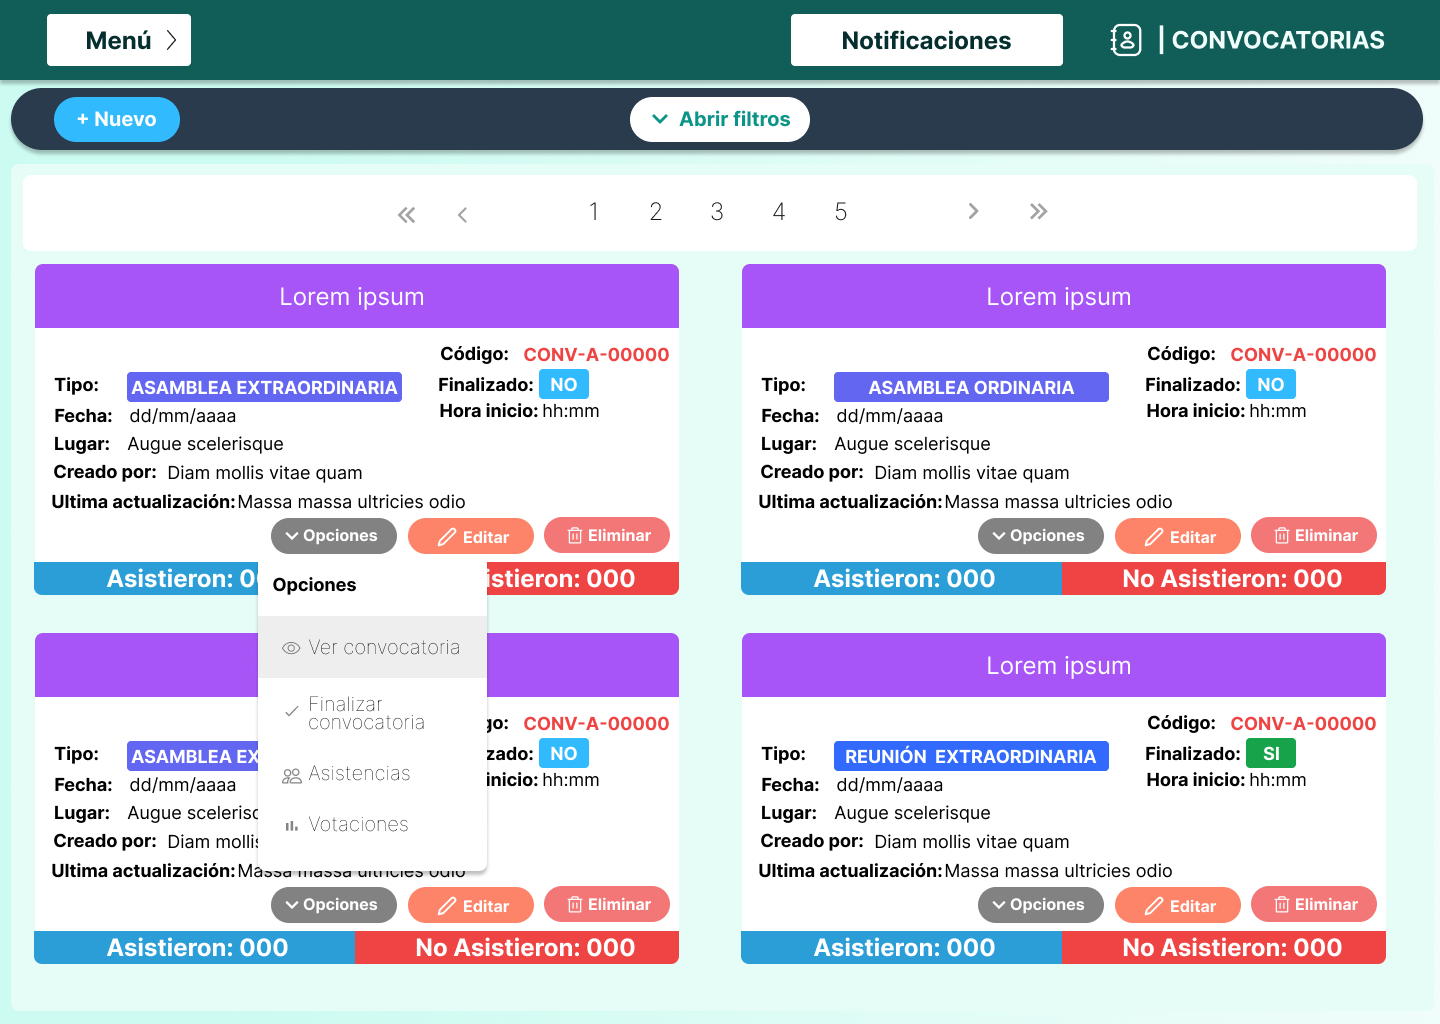
\includegraphics[width=1\textwidth]{resources/images/convocatorias}
    \caption{Prototipo de la vista de la administración de convocatorias}
    \label{fig:convocatorias}
\end{figure}

\begin{figure}[H]
    \centering
    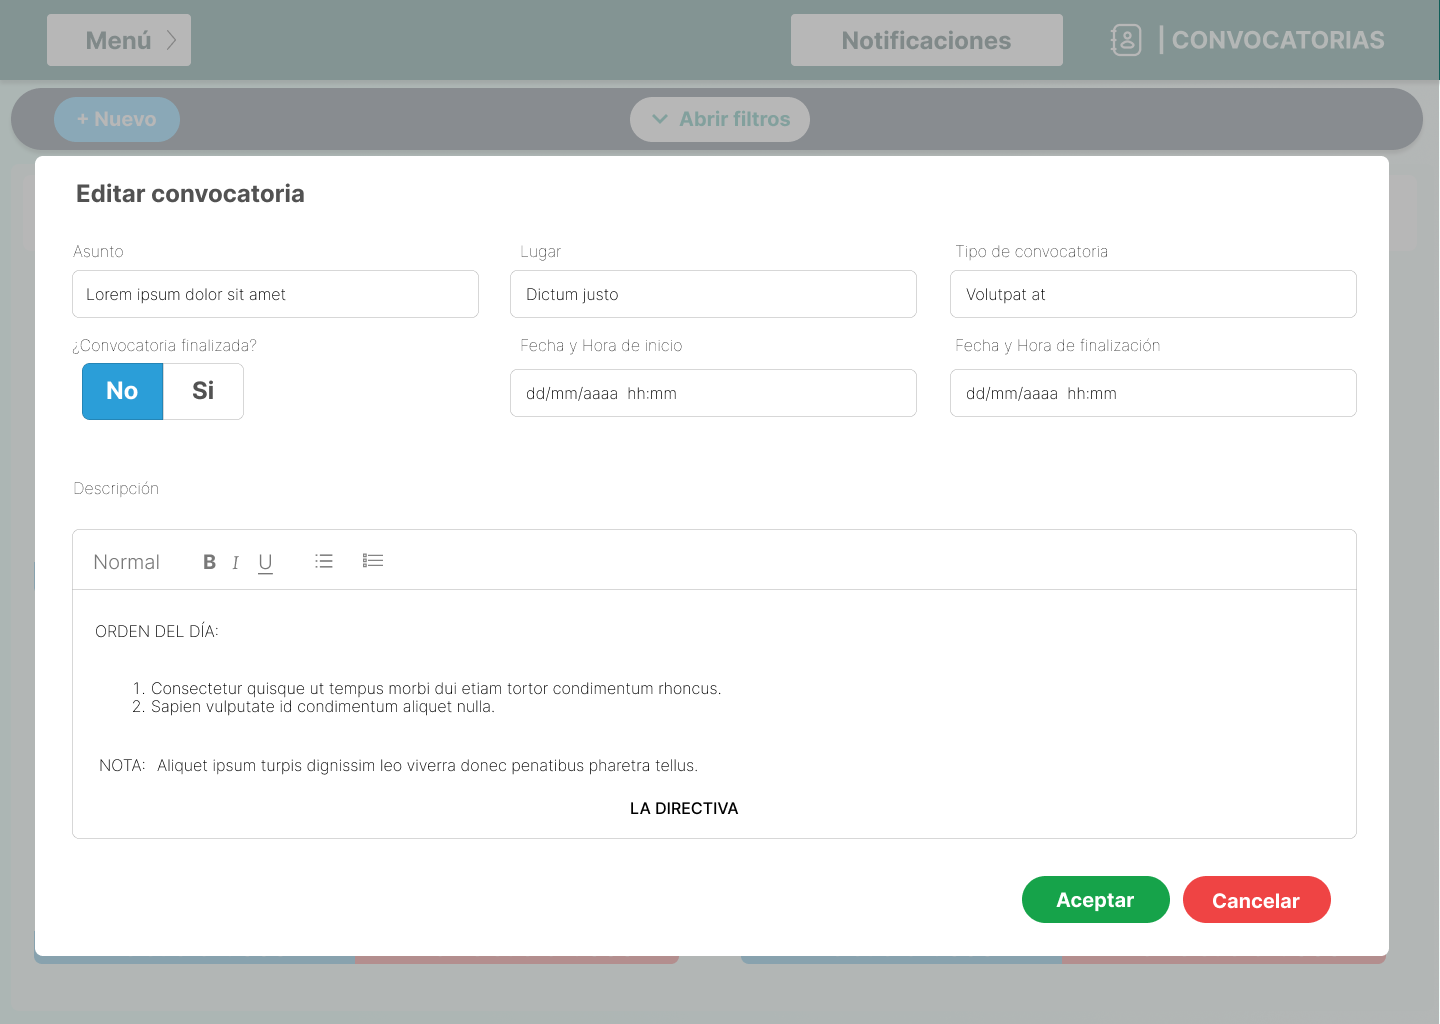
\includegraphics[width=1\textwidth]{resources/images/convocatorias_edit}
    \caption{Prototipo de la vista del formulario de de edición o creación de convocatorias}
    \label{fig:convocatorias-edit}
\end{figure}

\begin{figure}[H]
    \centering
    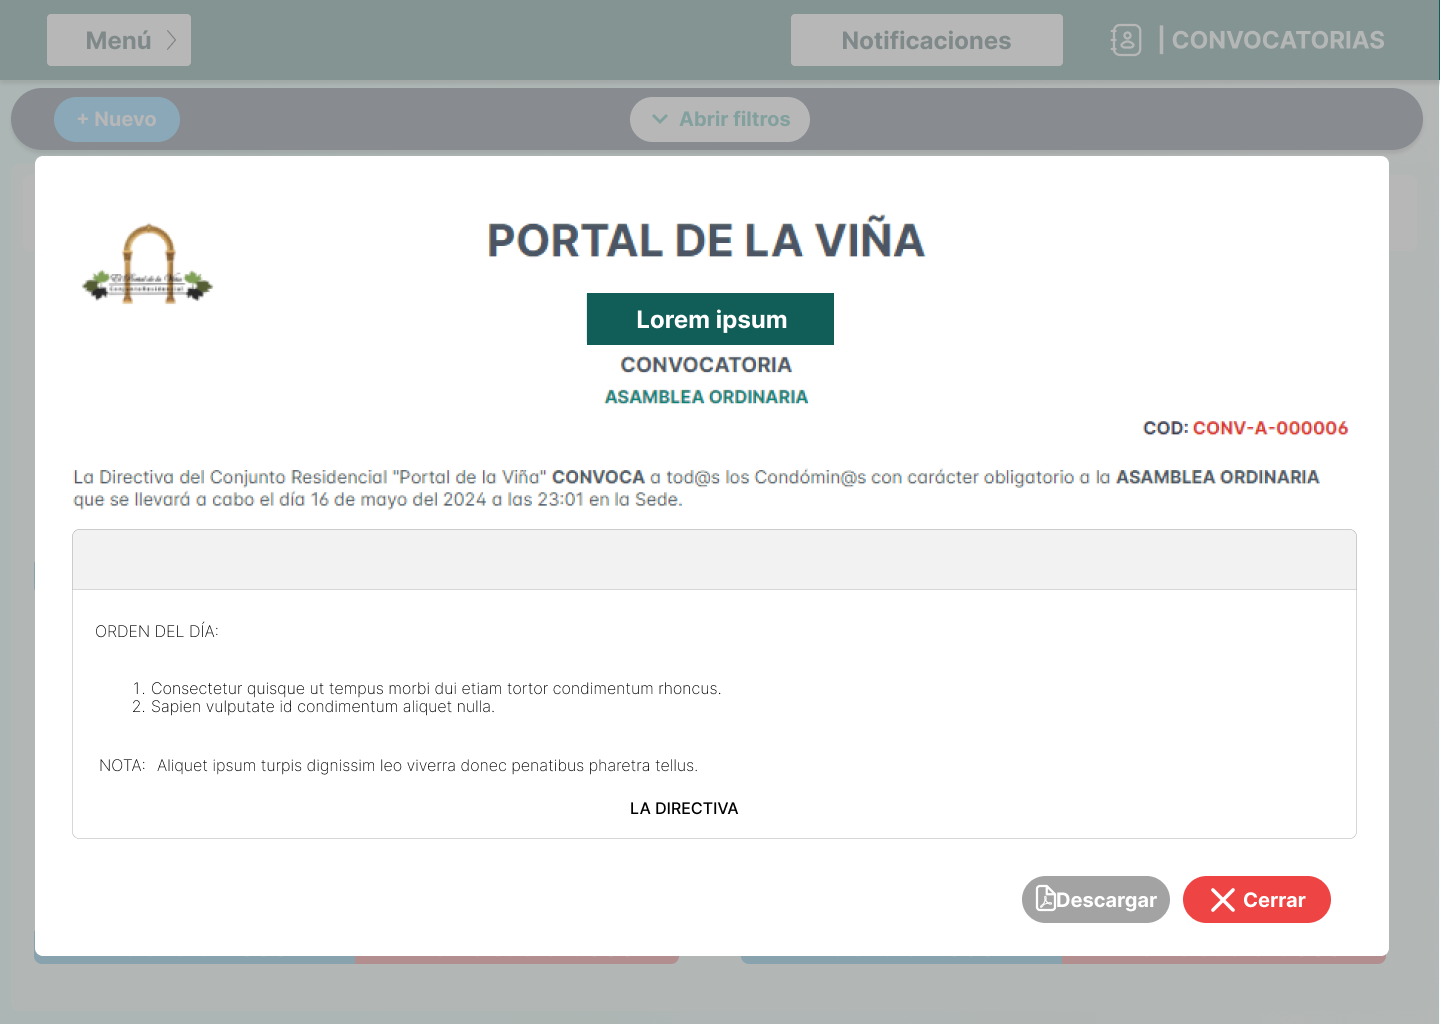
\includegraphics[width=1\textwidth]{resources/images/convocatorias_ver}
    \caption{Prototipo de la vista de vista previa a la descarga de la convocatoria}
    \label{fig:convocatorias-ver}
\end{figure}

\begin{figure}[H]
    \centering
    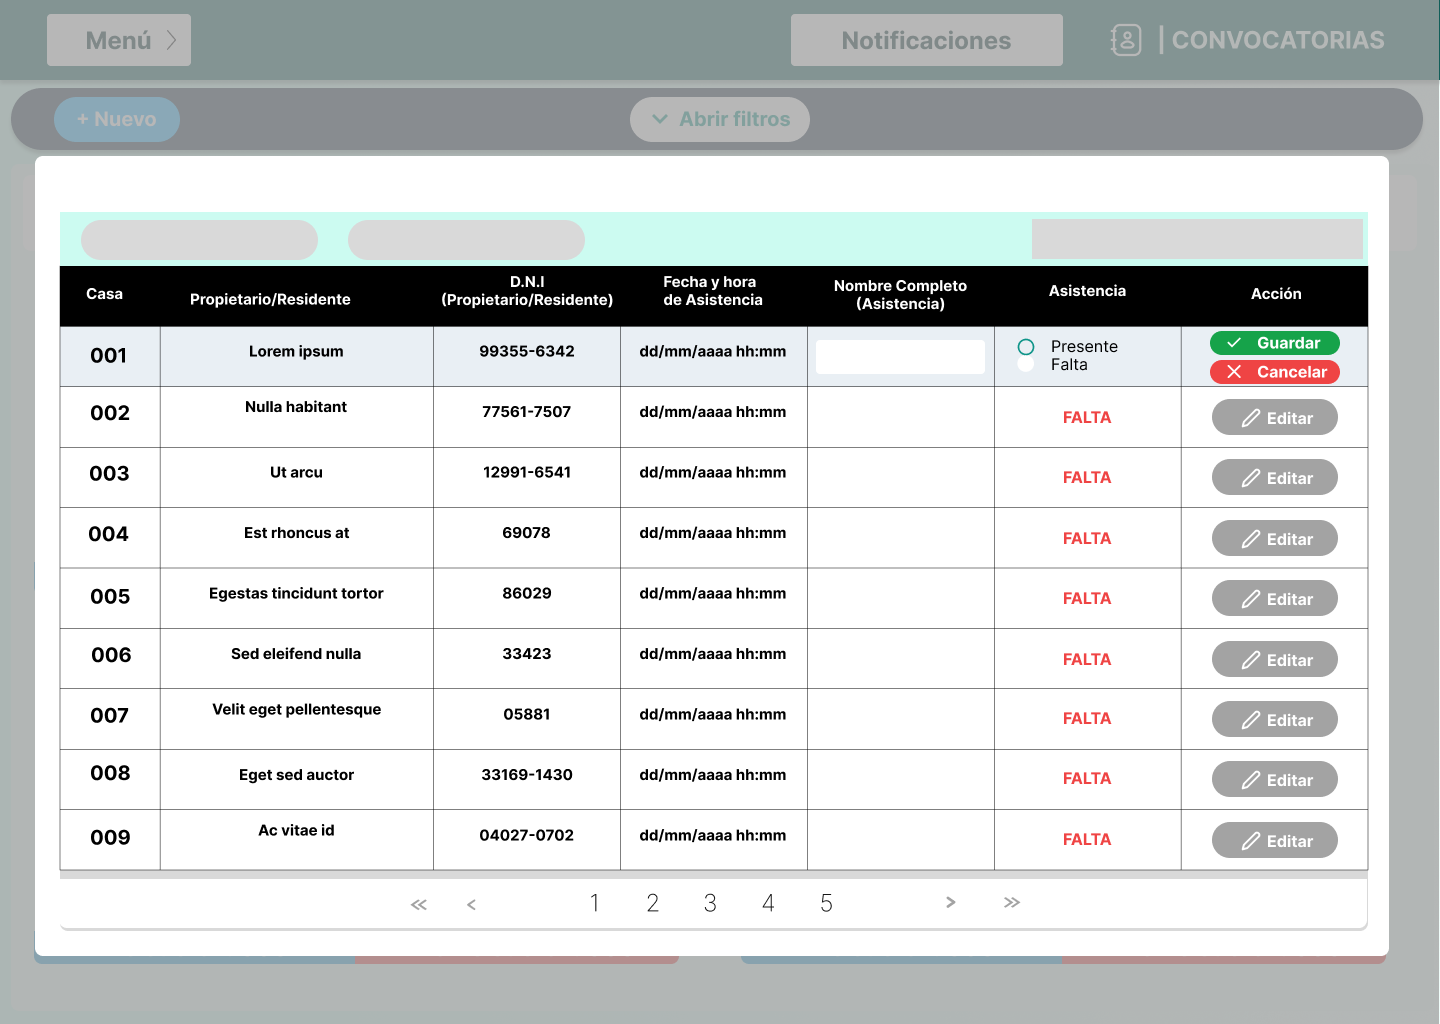
\includegraphics[width=1\textwidth]{resources/images/convocatorias_asistentes}
    \caption{Prototipo de la vista de administración de asistencias en asambleas}
    \label{fig:convocatorias-asistentes}
\end{figure}

\begin{figure}[H]
    \centering
    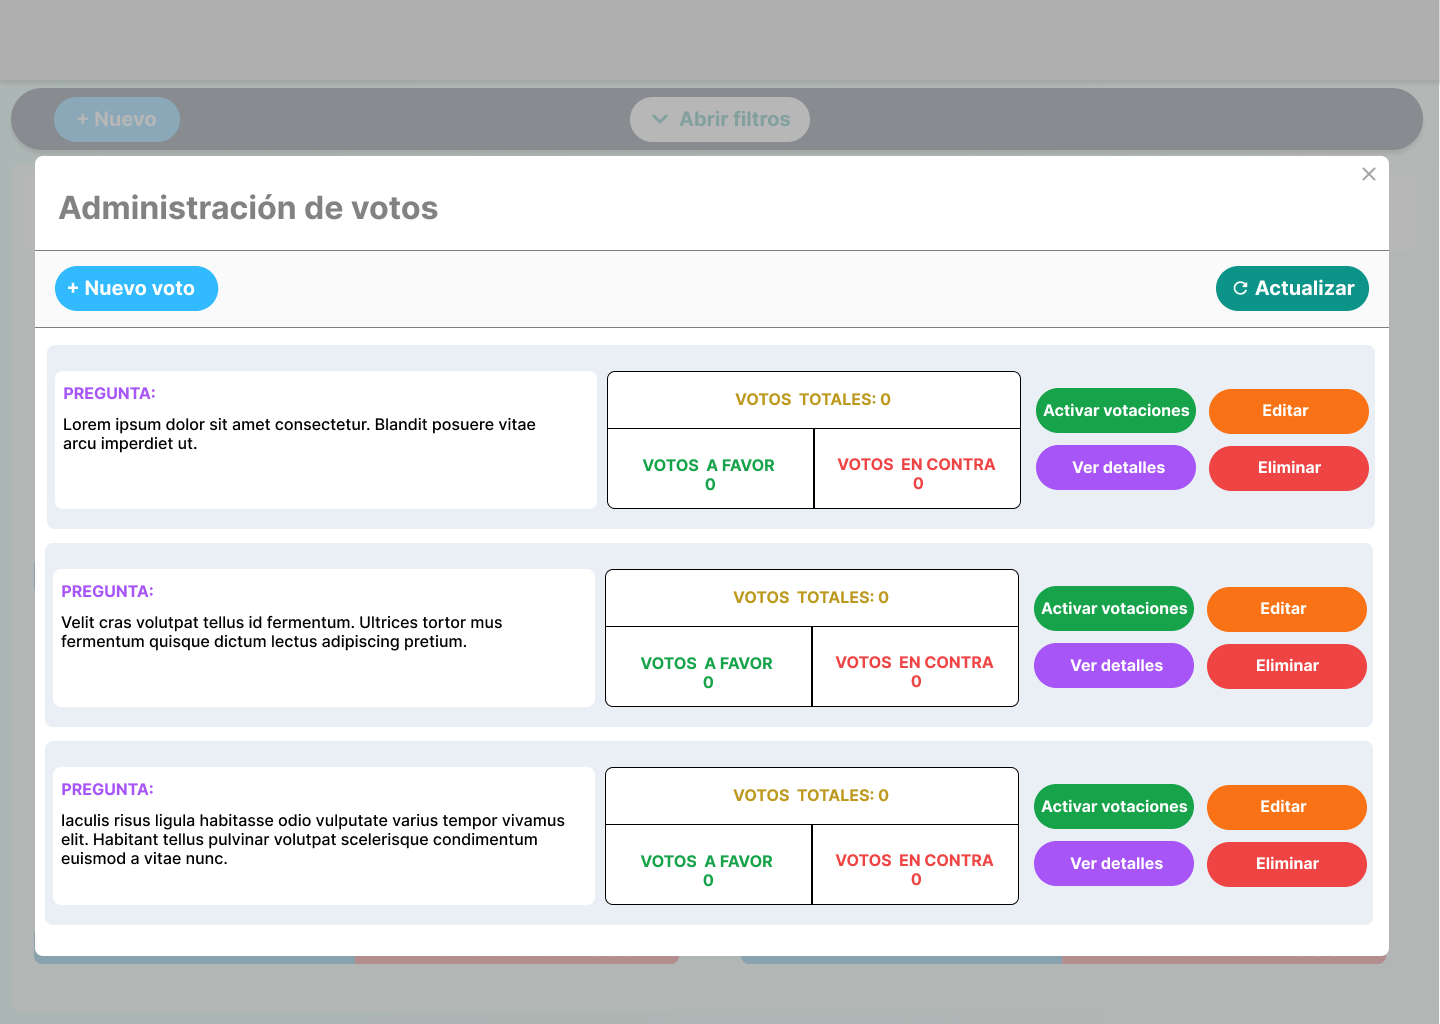
\includegraphics[width=1\textwidth]{resources/images/convocatorias_votaciones}
    \caption{Prototipo de la vista de administración de votaciones en asambleas}
    \label{fig:convocatorias-votaciones}
\end{figure}

En tesorería existen ingresos por tres conceptos los cuales son los ingresos casuales, mensuales y las multas, en la Figura \ref{fig:tesoreria-tipos} se muestra la vista de la administración de los tipos de ingresos mensuales y casuales con las todas las opciones de administración como la creación o edición de cada uno de los registros Figura \ref{fig:tesoreria-tipos-edit} y en la Figura \ref{fig:tesoreria-tipos-multas} se muestra la vista de la administración de los tipos de multas en donde también se visualizan todas las opciones de administración.


\begin{figure}[H]
    \centering
    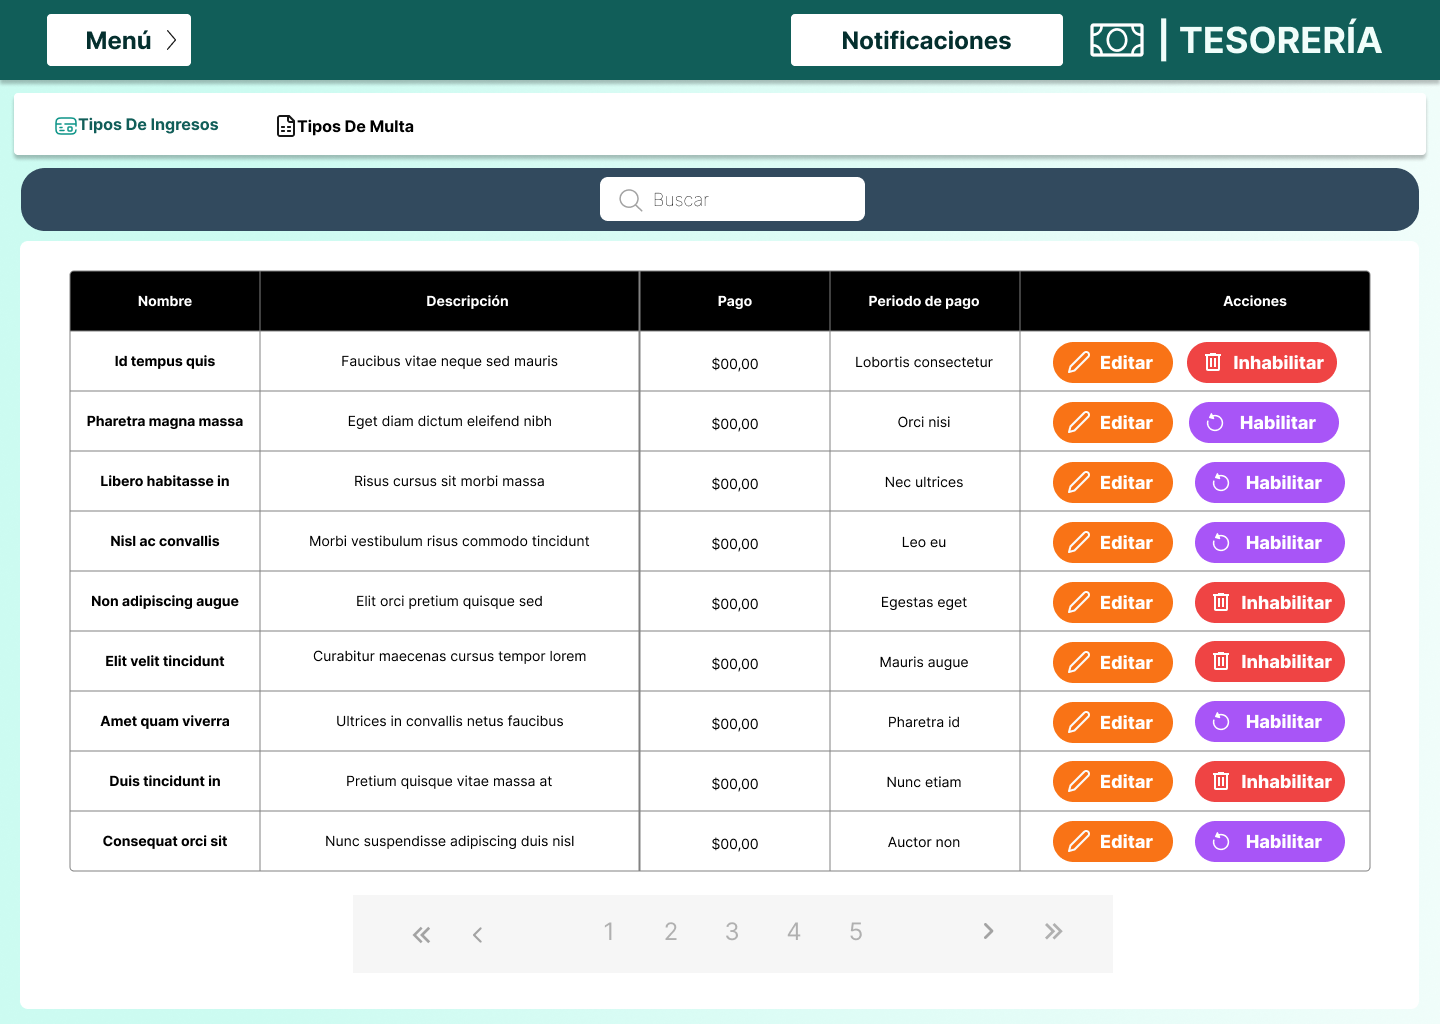
\includegraphics[width=1\textwidth]{resources/images/tesoreia - tipos}
    \caption{Prototipo de la vista de administración de tipos de ingresos casuales y mensuales}
    \label{fig:tesoreria-tipos}
\end{figure}

\begin{figure}[H]
    \centering
    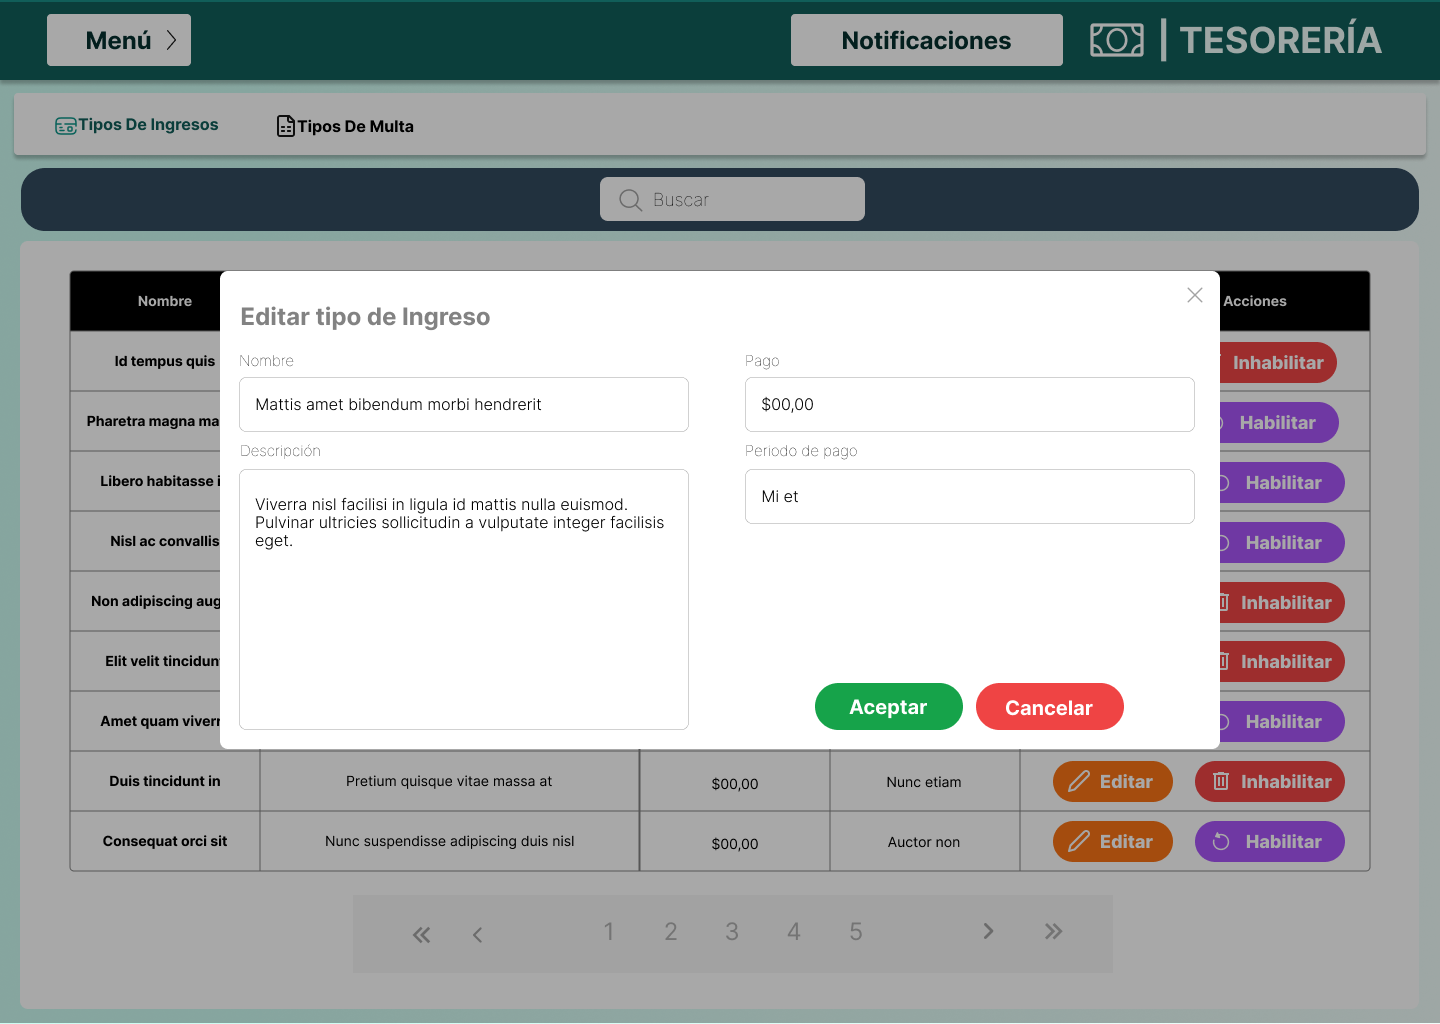
\includegraphics[width=1\textwidth]{resources/images/tesoreia - tipos edit}
    \caption{Prototipo de la vista del formulario de creación y edición de tipos de ingresos casuales y mensuales}
    \label{fig:tesoreria-tipos-edit}
\end{figure}

\begin{figure}[H]
    \centering
    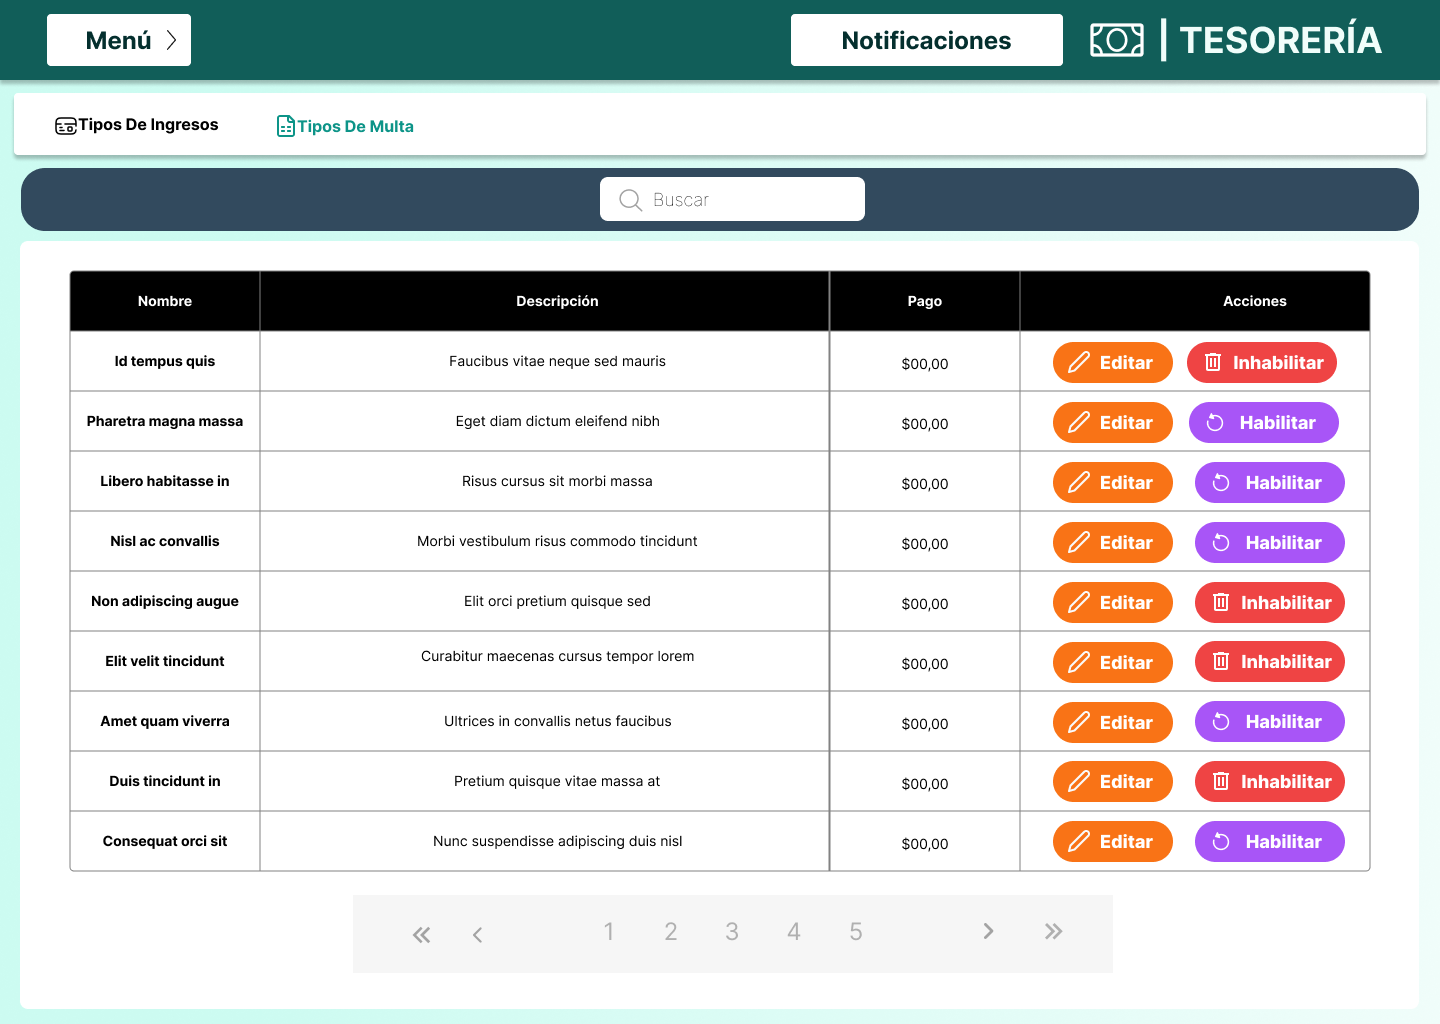
\includegraphics[width=1\textwidth]{resources/images/tesoreia - multas}
    \caption{Prototipo de la vista de administración de tipos de multas}
    \label{fig:tesoreria-tipos-multas}
\end{figure}

Tal como se muestra en la Figura \ref{fig:tesoreria-ingresos-mensuales} en los ingresos mensuales se visualizan los registros de los pagos realizados por los propietarios o inquilinos de alícuotas o parqueaderos azules junto con una imagen del comprobante de pago por parte de los mismos, para la creación o edición de los registros se despliega un formulario Figura \ref{fig:tesoreria-ingresos-mensuales-formulario} en donde se debe seleccionar la casa a la que se le va a realizar el registro del pago, en donde se colocará de forma automática el próximo mes a pagar y se podrá colocar hasta que fecha se realiza el pago, además de subir el comprobante de pago.
Por último en la Figura \ref{fig:tesoreria-ingresos-mensuales-recibo} se muestra la vista del recibo de cobro de los ingresos mensuales la cual puede ser descargada en formato PDF para su firma y envío al propietario o inquilino en el caso de ser necesario.

\begin{figure}[H]
    \centering
    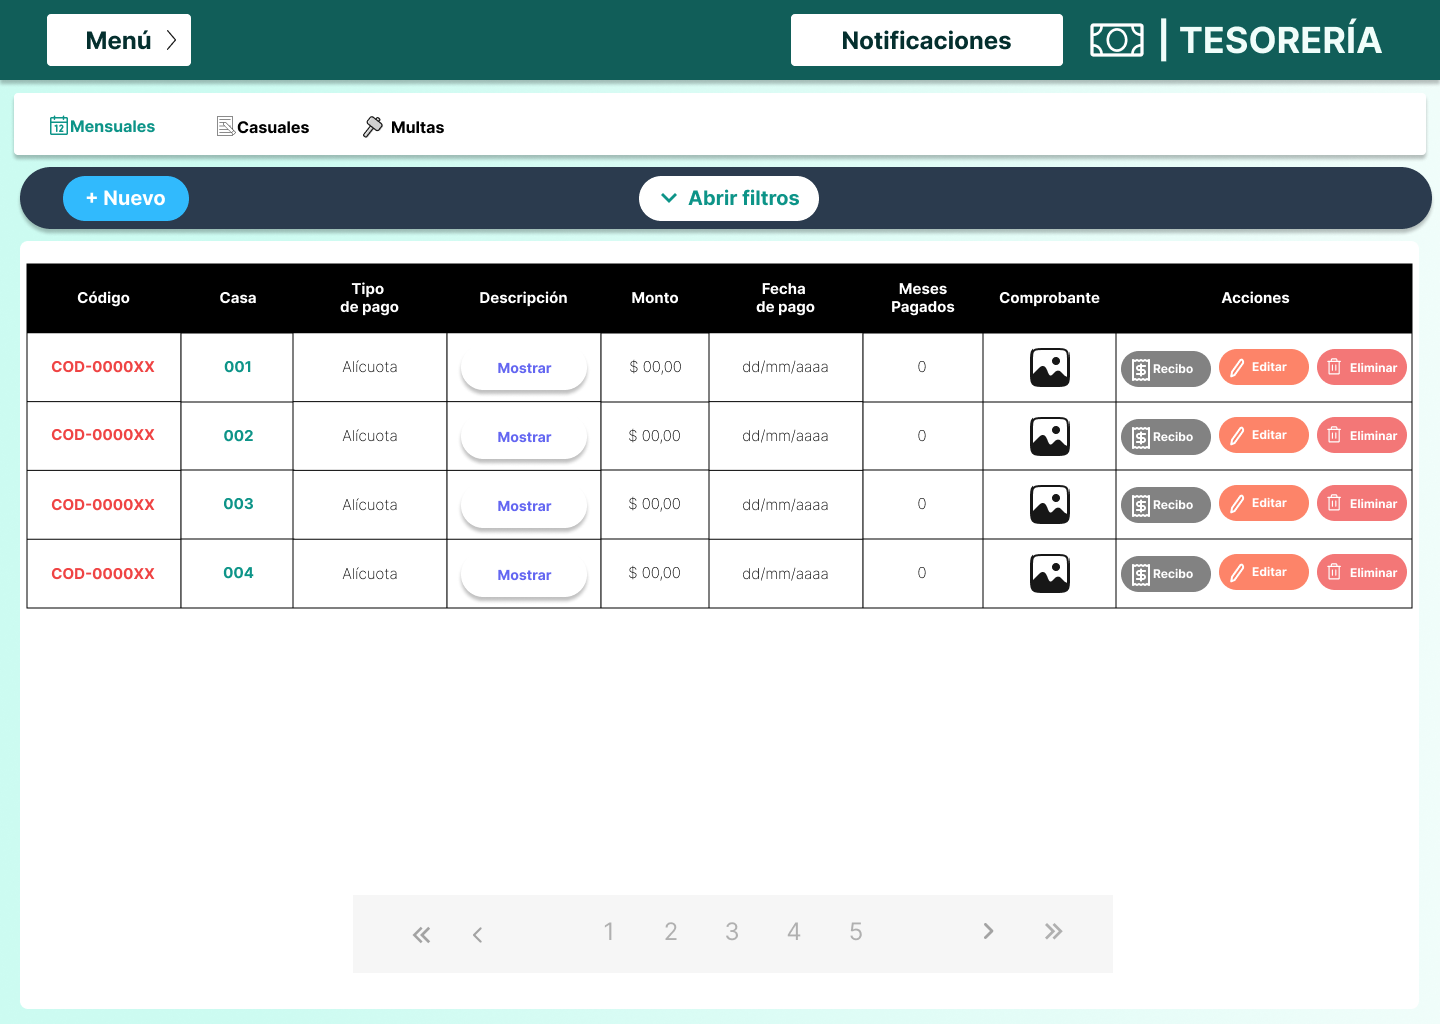
\includegraphics[width=1\textwidth]{resources/images/tesoreia - ingresos - mensuales}
    \caption{Prototipo de la vista de administración de ingresos mensuales}
    \label{fig:tesoreria-ingresos-mensuales}
\end{figure}

\begin{figure}[H]
    \centering
    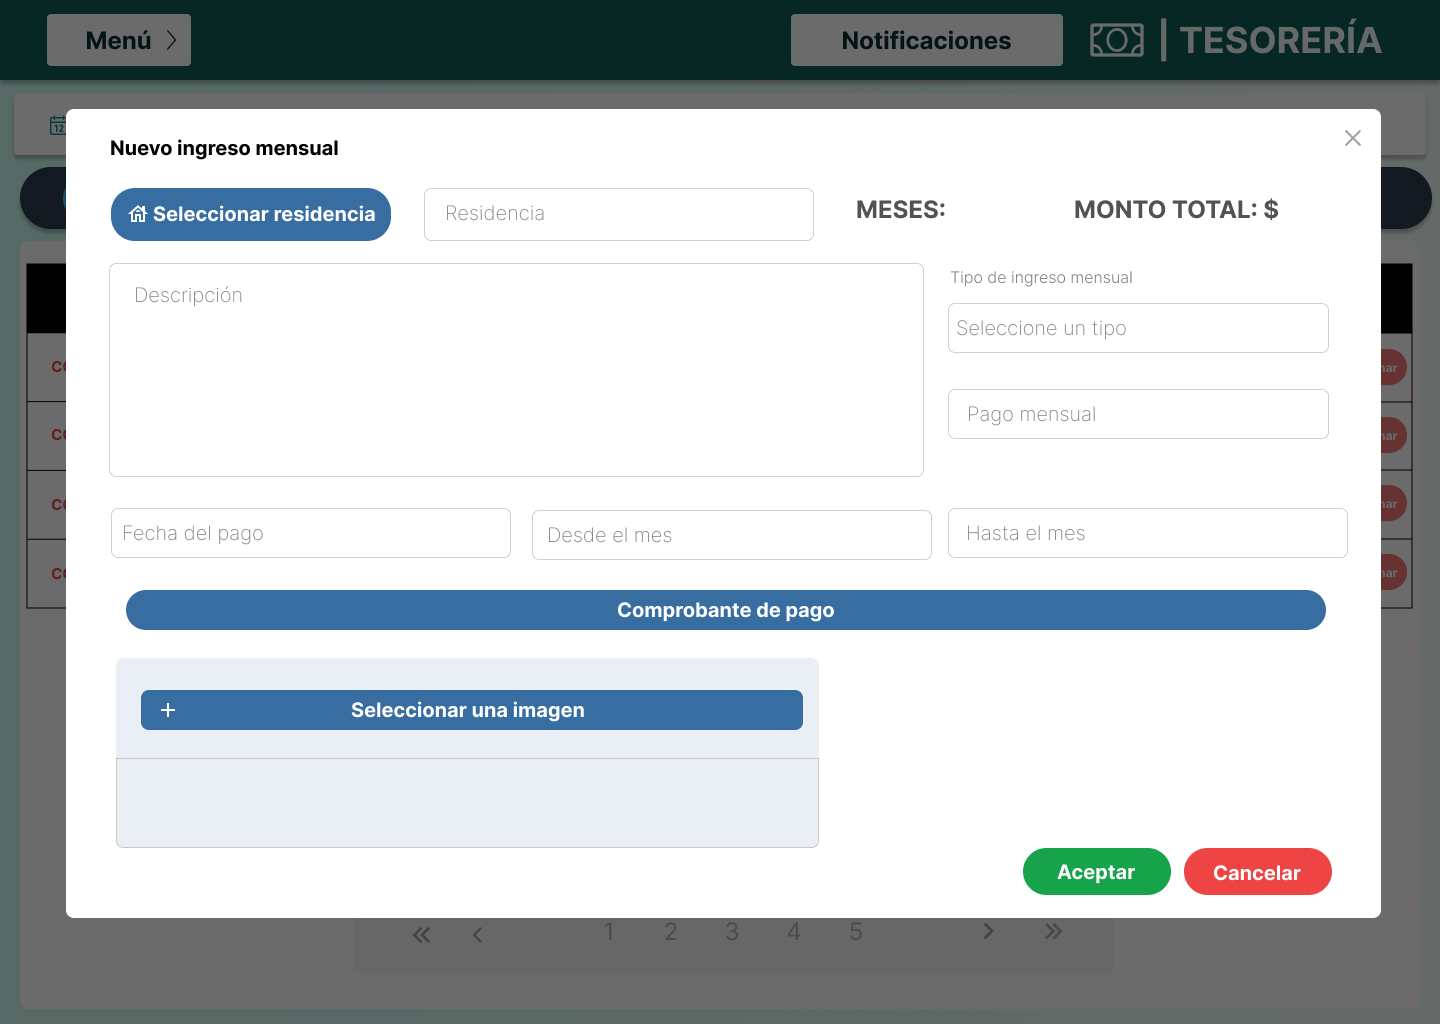
\includegraphics[width=1\textwidth]{resources/images/tesoreia - ingresos - mensuales - edit}
    \caption{Prototipo de la vista del formulario de creación y edición de ingresos mensuales}
    \label{fig:tesoreria-ingresos-mensuales-formulario}
\end{figure}

\begin{figure}[H]
    \centering
    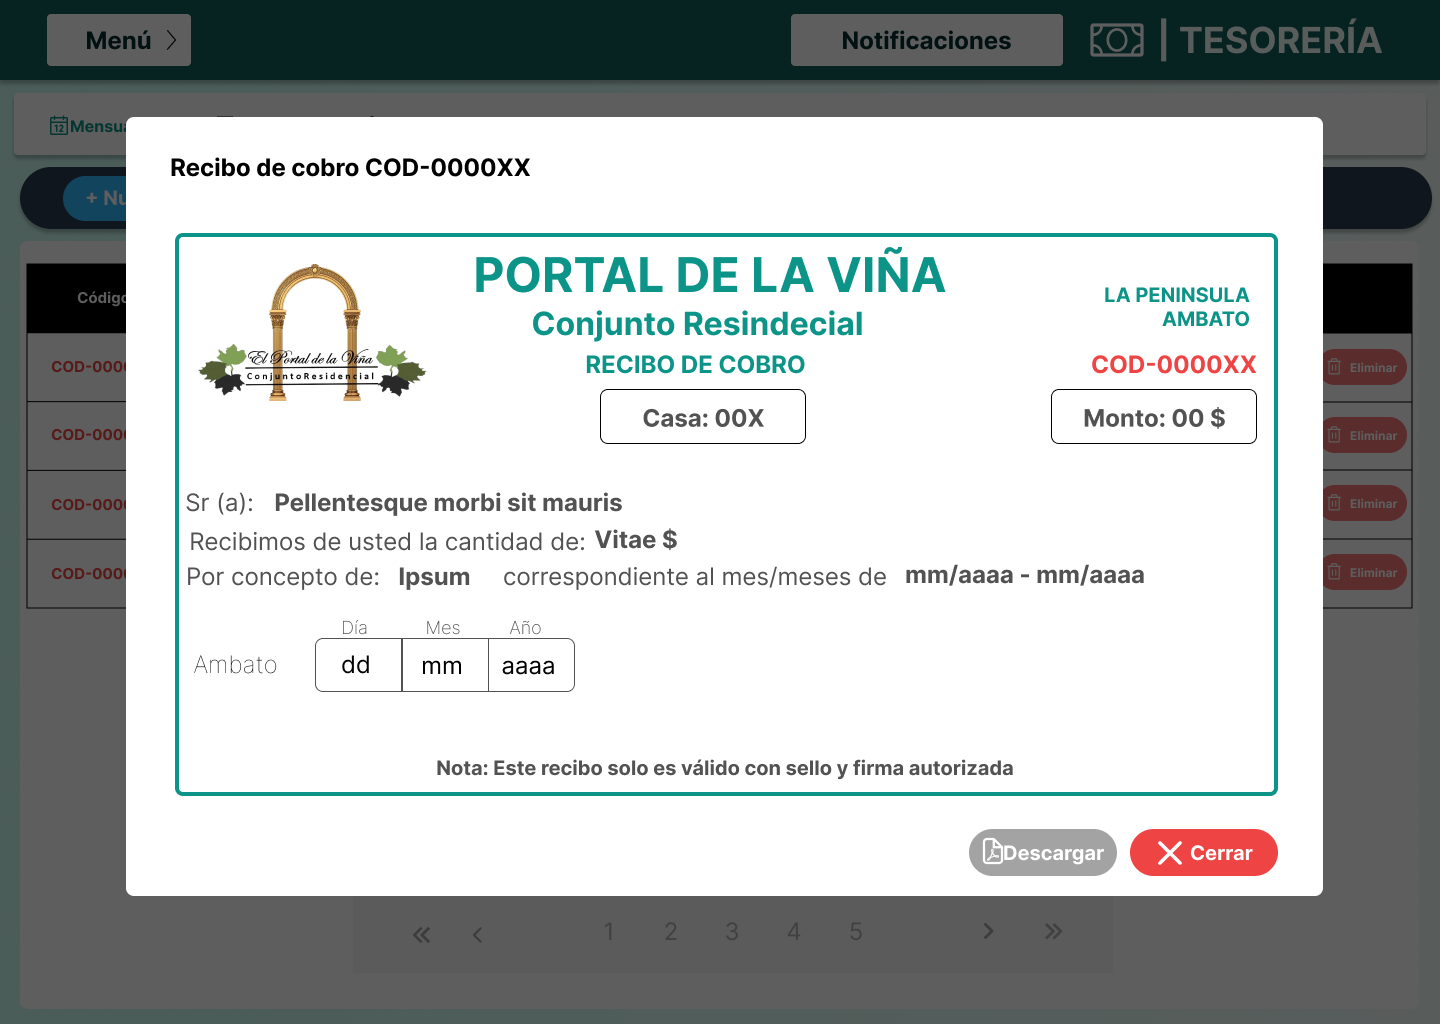
\includegraphics[width=1\textwidth]{resources/images/tesoreia-ingresos-mensuales-recibo}
    \caption{Prototipo de la vista del recibo de cobro generado por el sistema}
    \label{fig:tesoreria-ingresos-mensuales-recibo}
\end{figure}

En el caso de las múltas, son administradas de una forma muy similar a los pagos mensuales salvo que no tienen un rango de fechas de pago, en la Figura \ref{fig:tesoreria-ingresos-multas} se muestra el listado de registros de pagos de multas en los cuales se puede revisar el estado de las mismas para verificar si están pagadas o no, las evidencias de la multa y el comprobante de pago por parte del residente.
Para crear o editar un registro se despliega un formulario Figura \ref{fig:tesoreria-ingresos-multas-formulario} en donde se selecciona la residencia que será multada, el tipo de multa, junto con la fecha de la infracción, opcionalmente se pueden subir las evidencias y el comprobante de pago si en el caso de que sea una multa que ya se ha pagado para posteriormente generar un recibo de cobro de multa en formato PDF que ya se mostró en el proceso anterior Figura \ref{fig:tesoreria-ingresos-mensuales-recibo}.

\begin{figure}[H]
    \centering
    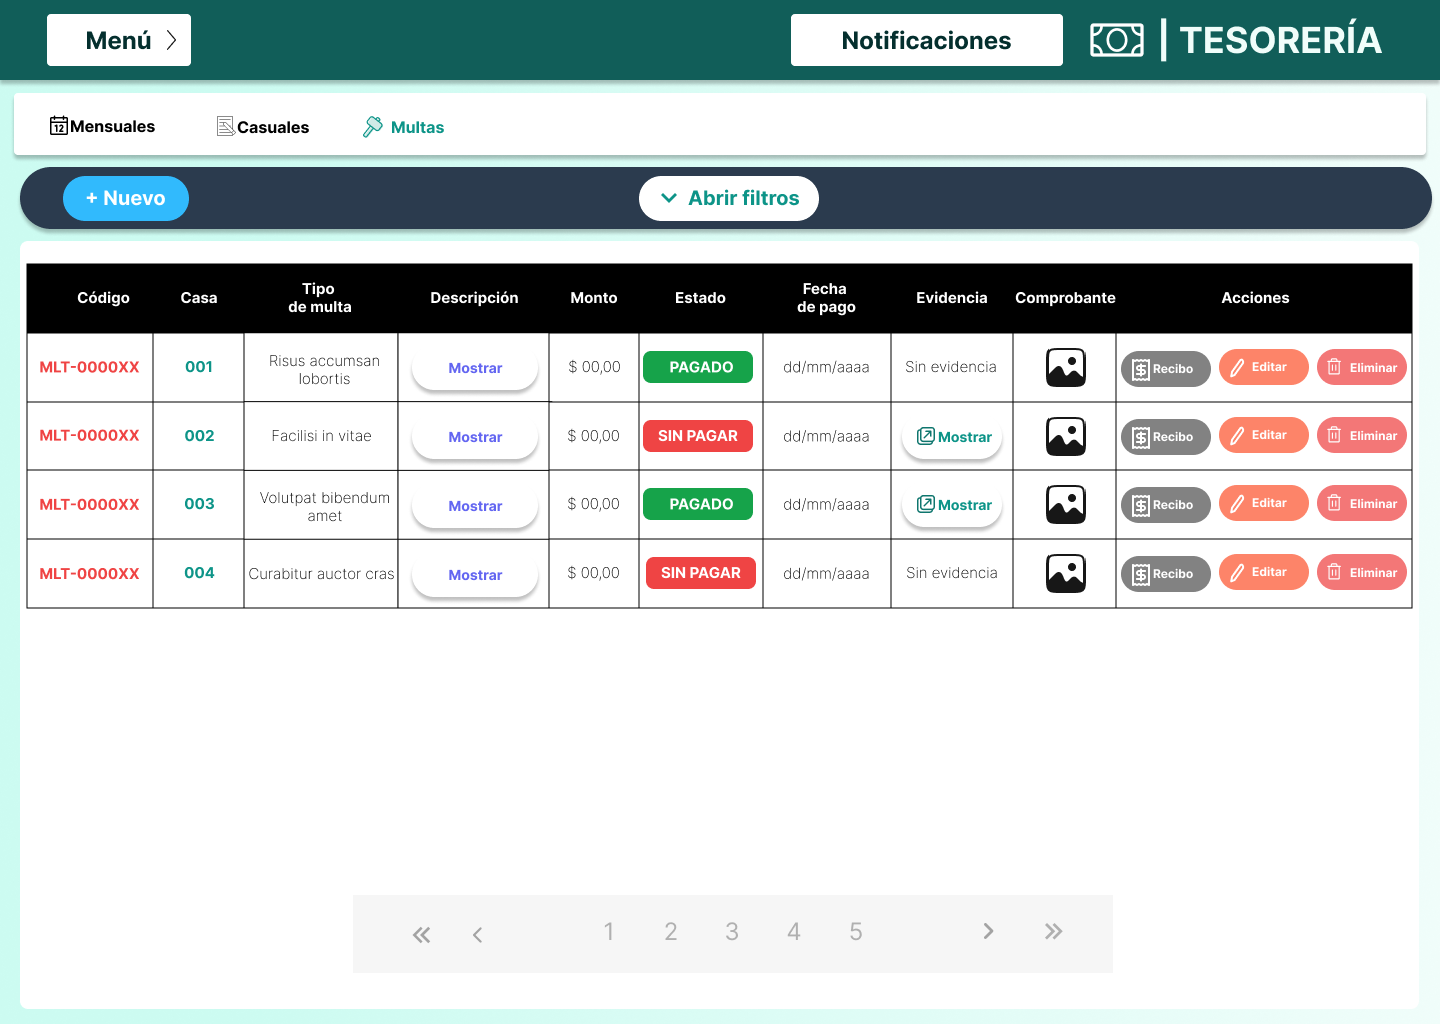
\includegraphics[width=1\textwidth]{resources/images/tesoreia - ingresos - multas}
    \caption{Prototipo de la vista de la administración de multas}
    \label{fig:tesoreria-ingresos-multas}
\end{figure}

\begin{figure}[H]
    \centering
    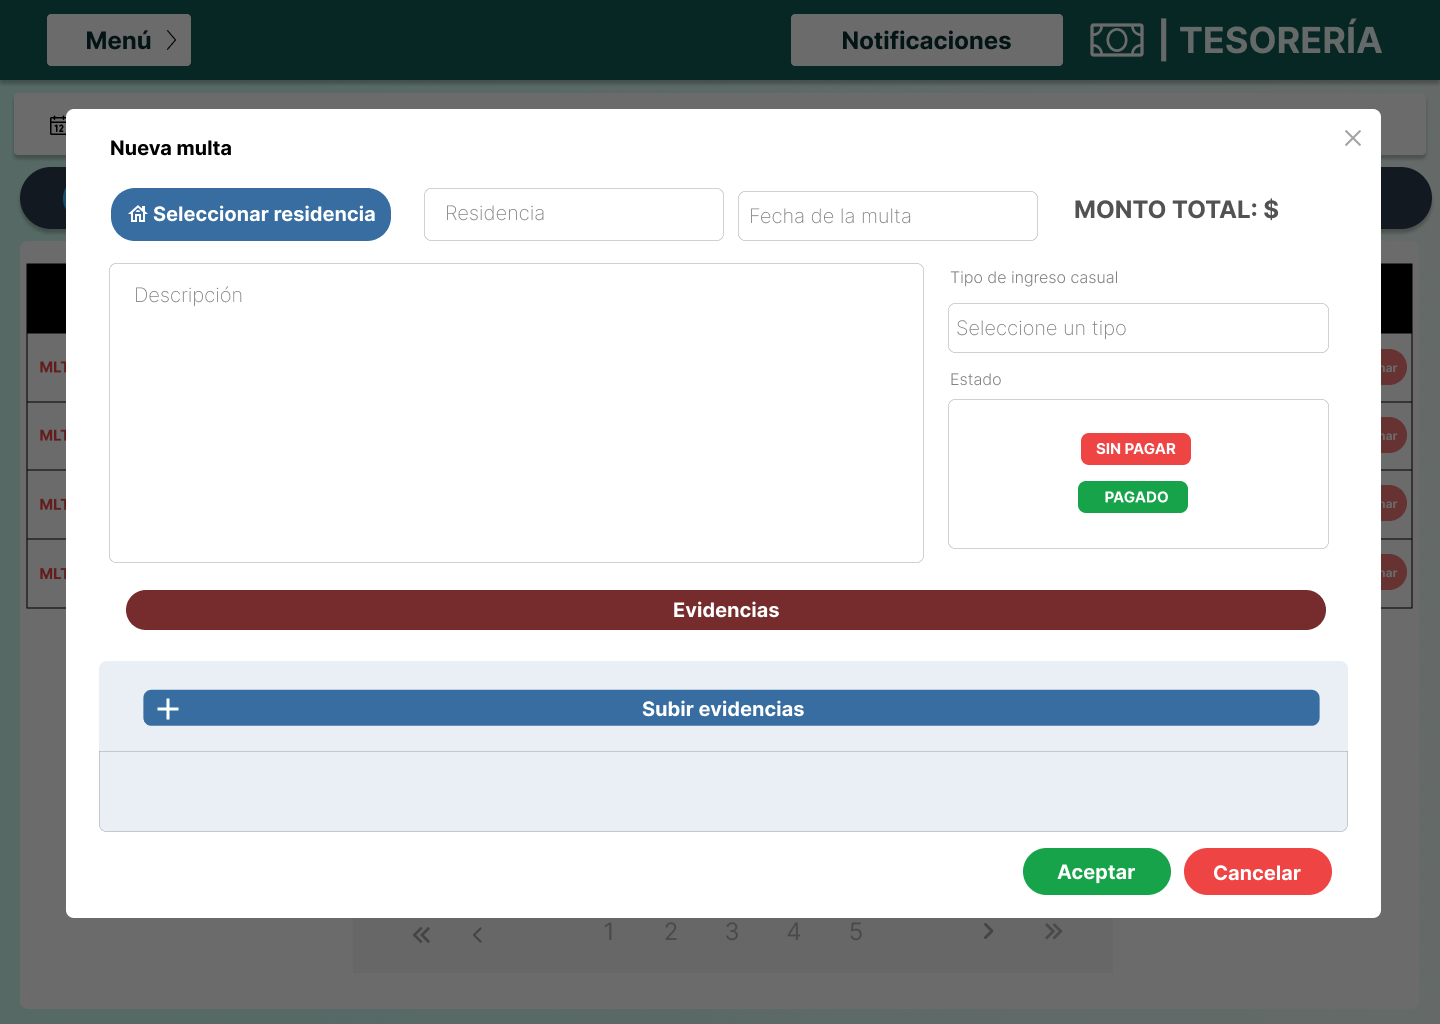
\includegraphics[width=1\textwidth]{resources/images/tesoreia - ingresos - multas -formulario}
    \caption{Prototipo de la vista del formulario de creación y edición de ingresos multas}
    \label{fig:tesoreria-ingresos-multas-formulario}
\end{figure}

Para el registro de egresos en la Figura \ref{fig:tesoreria-egresos} se muestra la vista administradora de los egresos en los cuales se pueden visualizar, registrar o editar los registros de los pagos a proveedores o eliminarlos en caso de ser necesario.
Posteriormente a este proceso se tienen la administración de los tipos de egresos Figura \ref{fig:tesoreria-egresos-tipos} y también la administración de los proveedores Figura \ref{fig:tesoreria-egresos-proveedores} en donde en ambos casos se pueden visualizar, registrar, editar o inhabilitar.
Continuando con los egresos en la Figura \ref{fig:tesoreria-egresos-formulario} se muestra la vista del formulario para edición o registro en donde se necesita seleccionar el proveedor, el tipo de egreso, la fecha de la factura, el monto registrado en la factura, la factura o comprobante expendida por el proveedor y una descripción del egreso.

\begin{figure}[H]
    \centering
    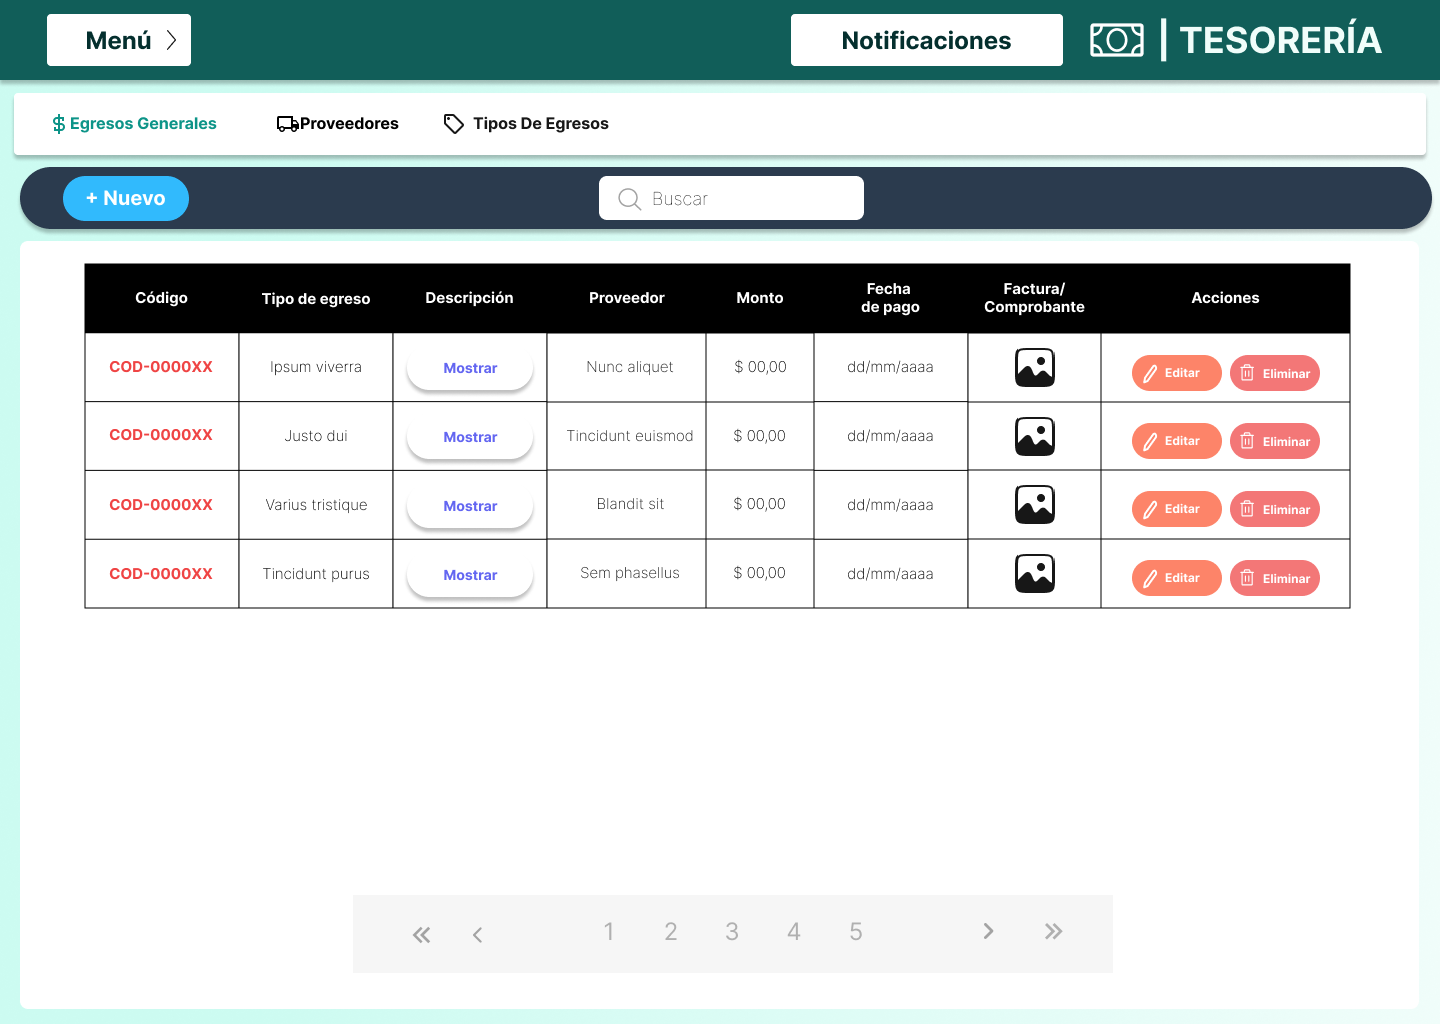
\includegraphics[width=1\textwidth]{resources/images/tesoreia - egresos - generales}
    \caption{Prototipo de la vista de la administración de egresos}
    \label{fig:tesoreria-egresos}
\end{figure}

\begin{figure}[H]
    \centering
    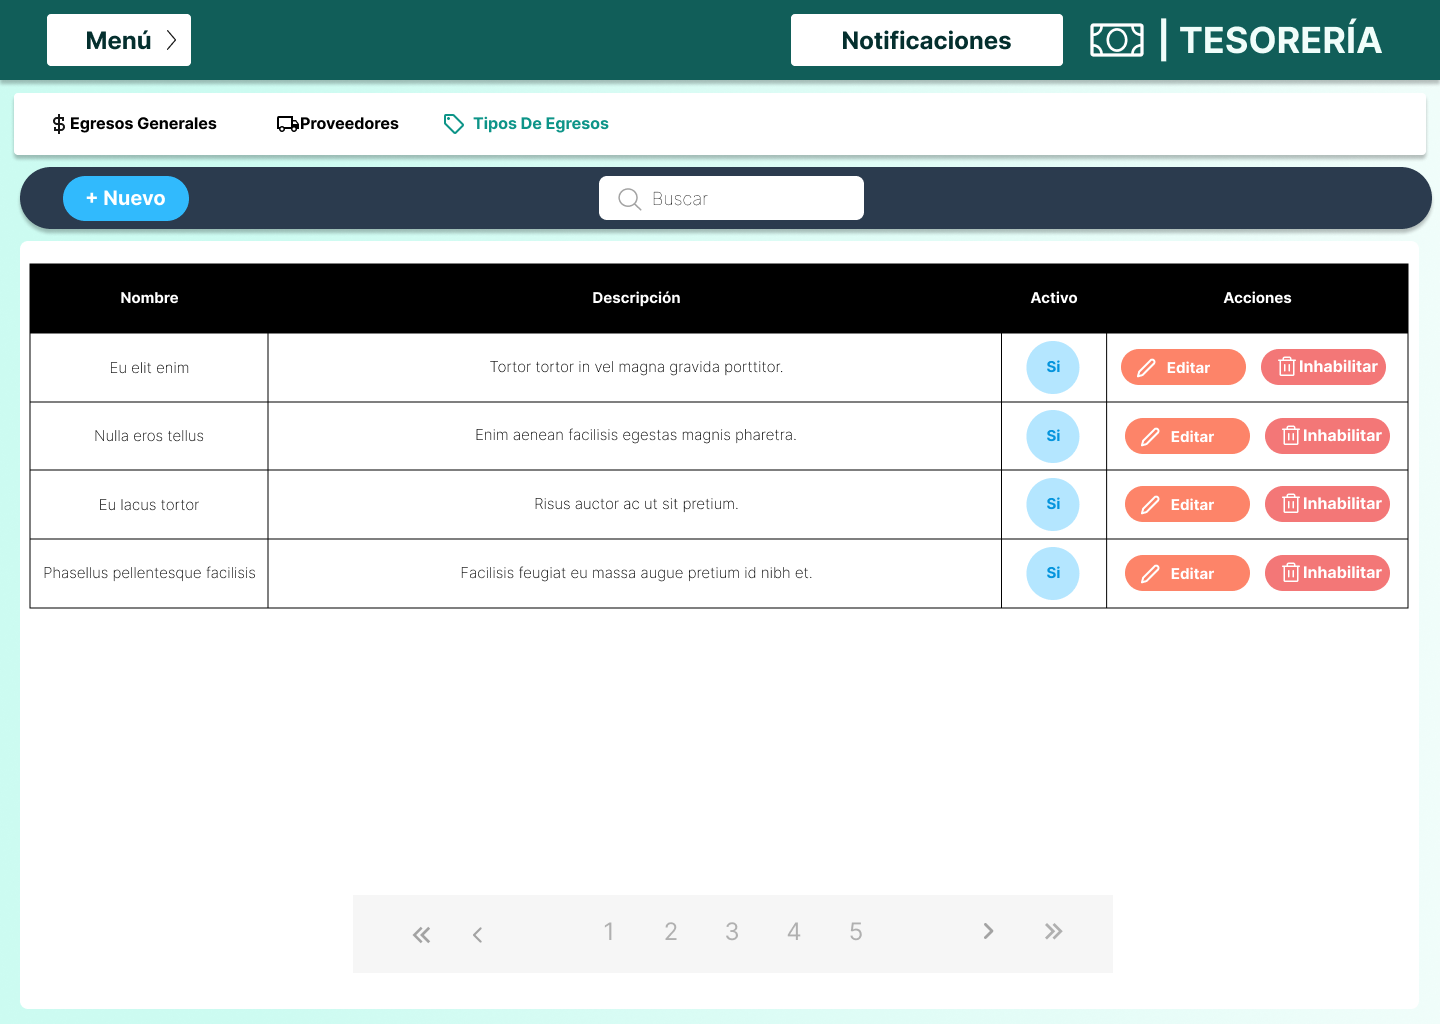
\includegraphics[width=1\textwidth]{resources/images/tesoreia - egresos - tipos}
    \caption{Prototipo de la vista de la administración de tipos de egresos}
    \label{fig:tesoreria-egresos-tipos}
\end{figure}

\begin{figure}[H]
    \centering
    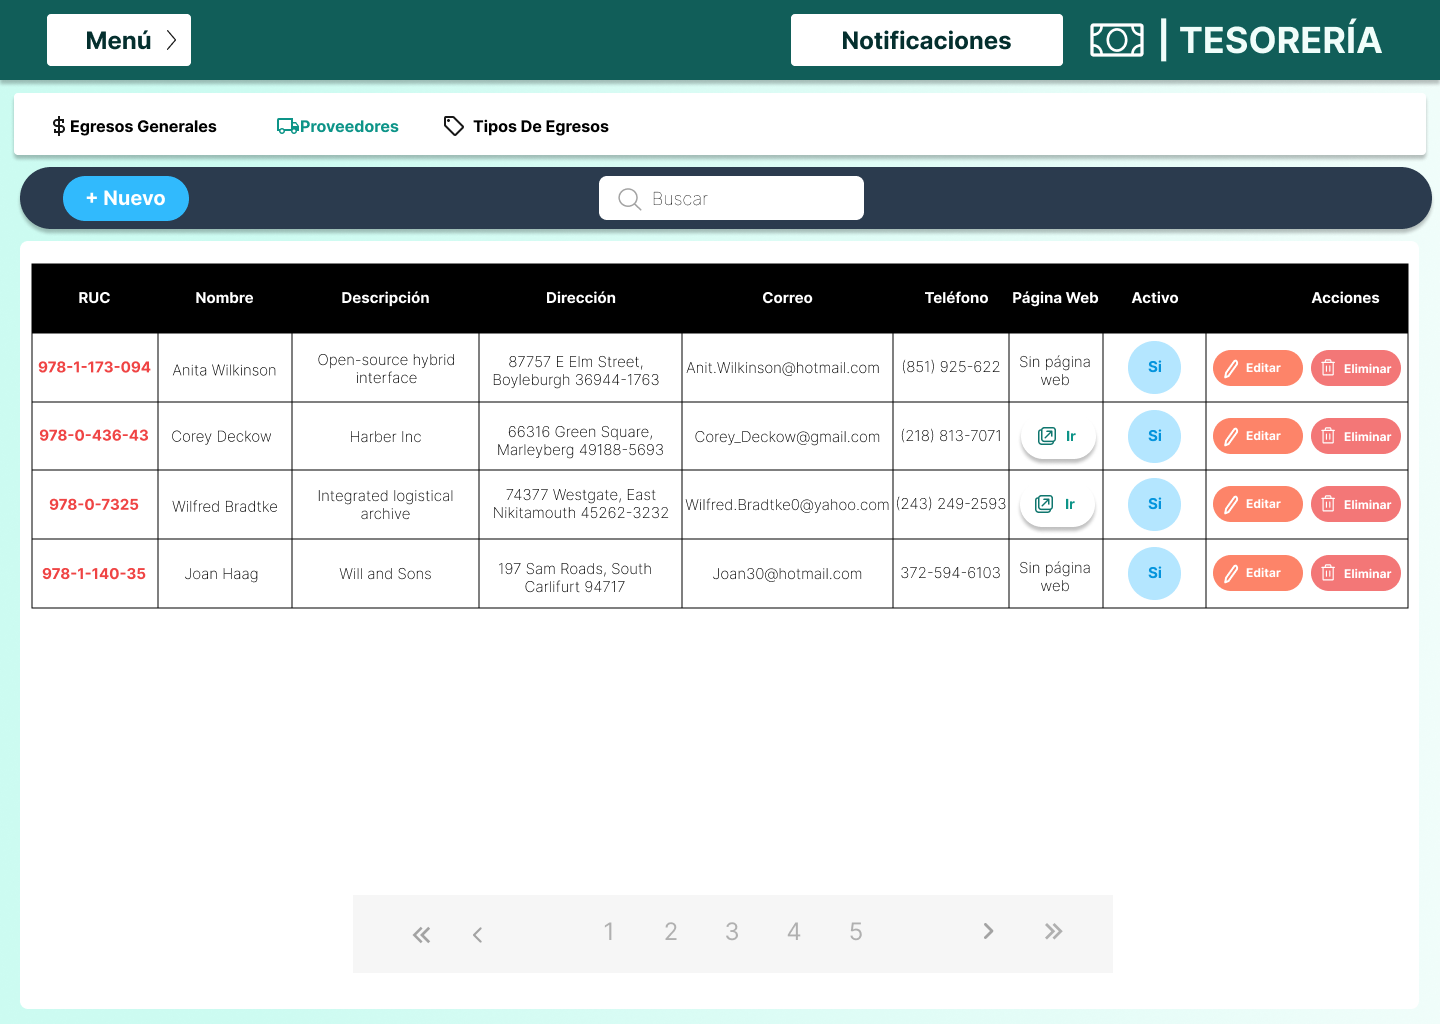
\includegraphics[width=1\textwidth]{resources/images/tesoreia - egresos - proveedores}
    \caption{Prototipo de la vista de la administración de proveedores}
    \label{fig:tesoreria-egresos-proveedores}
\end{figure}

\begin{figure}[H]
    \centering
    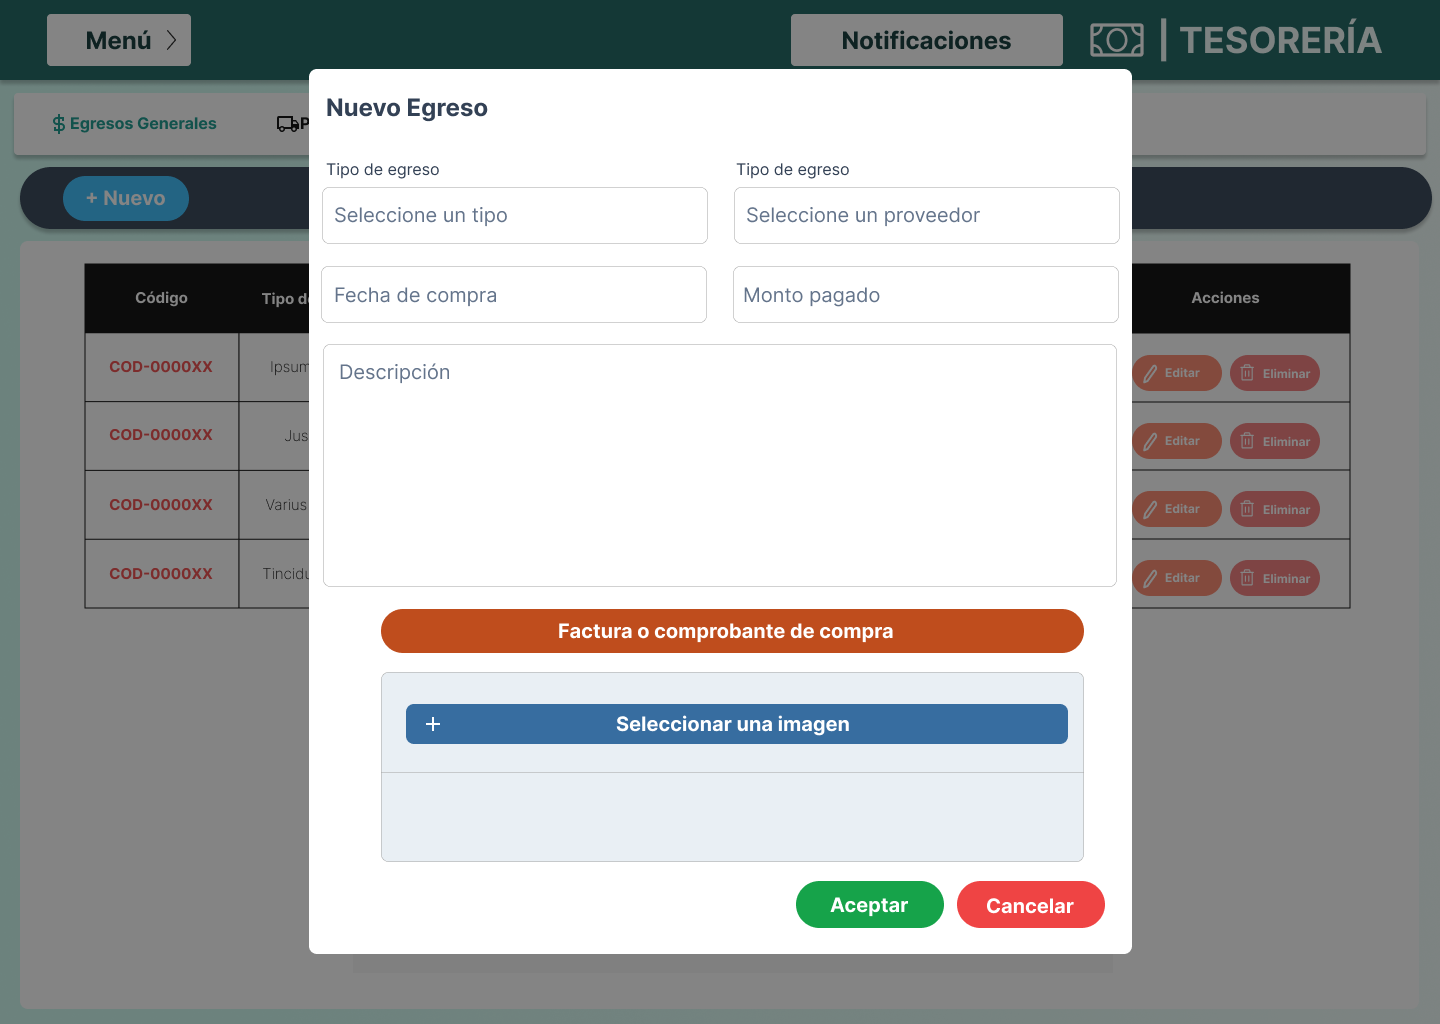
\includegraphics[width=1\textwidth]{resources/images/tesoreia - egresos - generales-edit}
    \caption{Prototipo de la vista del formulario de creación y edición de egresos}
    \label{fig:tesoreria-egresos-formulario}
\end{figure}

\textbf{Prototipo móvil}
\bigbreak

Para el inicio de sesión en la aplicación móvil tan como se muestra en la Figura \ref{fig:login-movil} el usuario debe proporcionar sus credenciales de acceso, además de también contar con la opción de poder recuperar la contraseña mediante su correo electrónico.

\begin{figure}[H]
    \centering
    \fbox{
\includegraphics[width=0.3\textwidth]{resources/images/Login-movil}}
    \caption{Prototipo de la vista del inicio de sesión}
    \label{fig:login-movil}
\end{figure}

En la parte inferior se puede ver la barra de navegación con las opciones del menú de la aplicación Figura \ref{fig:navegacion-movil} en donde se visualizan las opciones de eventos, hogar, asambleas y perfil.

\begin{figure}[H]
    \centering
    \fbox{
\includegraphics[width=0.3\textwidth]{resources/images/navegacion-movil}}
    \caption{Prototipo de la vista de la barra de navegación}
    \label{fig:navegacion-movil}
\end{figure}

Al iniciar sesión como primera vista se mostrarán los eventos próximos a realizarse en el condominio Figura \ref{fig:login-eventos}los cuales pueden ser eventos sociales o eventos de asambleas, adicionalmente se podrá ver de una forma más detallada la información de cada evento como se muestra en la Figura \ref{fig:login-eventos-detalle} en donde se visualiza la fecha, hora, lugar y descripción del evento.

\begin{figure}[H]
    \centering
    \fbox{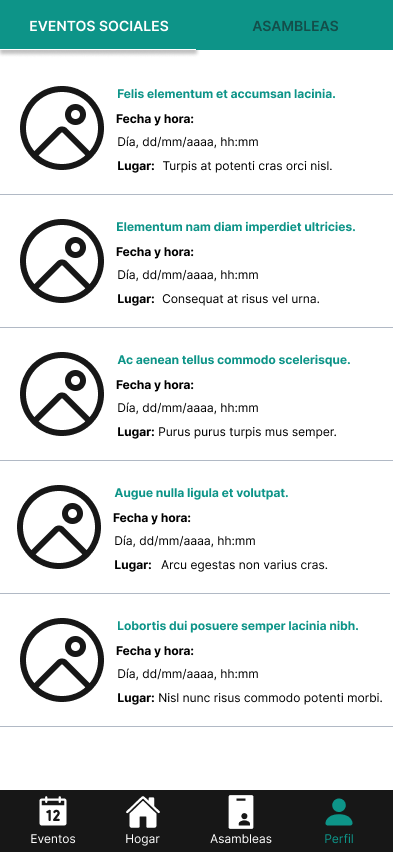
\includegraphics[width=0.3\textwidth]{resources/images/eventos-movil}}
    \caption{Prototipo de la vista de eventos próximos}
    \label{fig:login-eventos}
\end{figure}


\begin{figure}[H]
    \centering
    \fbox{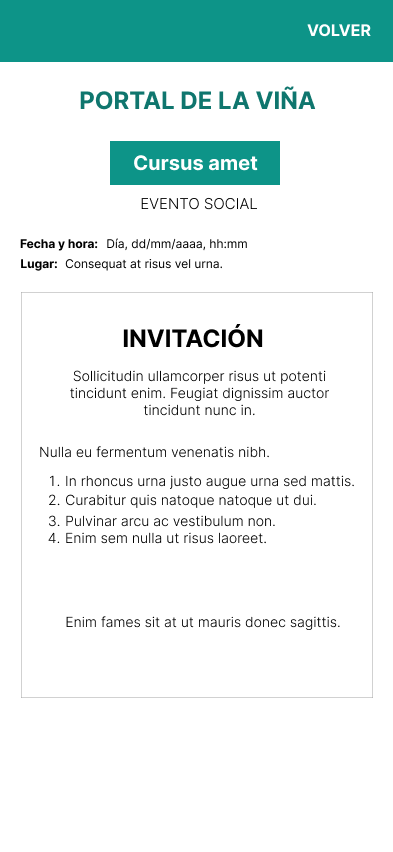
\includegraphics[width=0.3\textwidth]{resources/images/eventos-detalle}}
    \caption{Prototipo de la vista detallada de un evento}
    \label{fig:login-eventos-detalle}
\end{figure}

En la sección de asambleas se mostrará únicamente la asamblea que se dará lugar en el día actual Figura \ref{fig:asambleas-movil}, en donde se podrá visualizar la información más relevante como la fecha de inicio, la ficha límite pára poder registrar la asistencia, el lugar en donde se dará la asamblea y la opción de poder registrar o votar en la asamblea.


En el caso de querer registrar la asistencia se mostrará la o las residencias asociadas al usuario que ha iniciado sesión en donde tendrá que registrar su asistencia por cada una de sus residencias como se muestra en la Figura \ref{fig:asambleas-asistencia-movil}.
También se mostrarán en la parte superior indicaciones a tomar en cuenta para el registro de asistencia en la asamblea.


Por otro lado en el caso de que se quiera votar en la asamblea se mostrarán las preguntas a votar habilitadas por el presidente o vicepresidente en donde el usuario podrá decidir si esta a favor o en contra de la pregunta tal como se muestra en la Figura \ref{fig:asambleas-votacion-movil}.
Al igual que en el registro también para las votaciones se mostrarán indicaciones en la parte superior.

\begin{figure}[H]
    \centering
    \fbox{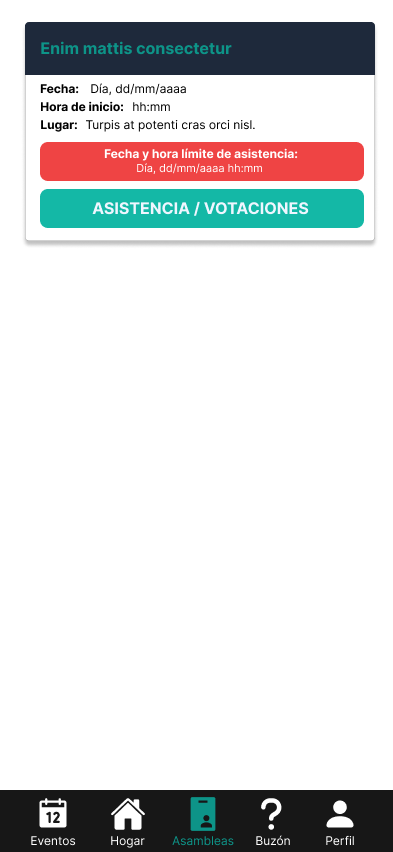
\includegraphics[width=0.3\textwidth]{resources/images/Asambleas-movil}}
    \caption{Prototipo de la vista de asambleas del día actual}
    \label{fig:asambleas-movil}
\end{figure}

\begin{figure}[H]
    \centering
    \fbox{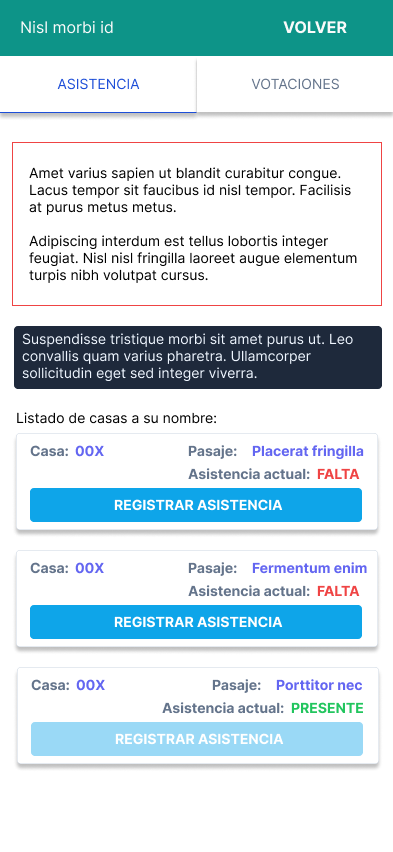
\includegraphics[width=0.3\textwidth]{resources/images/Asambleas-asistencia-movil}}
    \caption{Prototipo de la vista del registro de asistencia en asambleas}
    \label{fig:asambleas-asistencia-movil}
\end{figure}

\begin{figure}[H]
    \centering
    \fbox{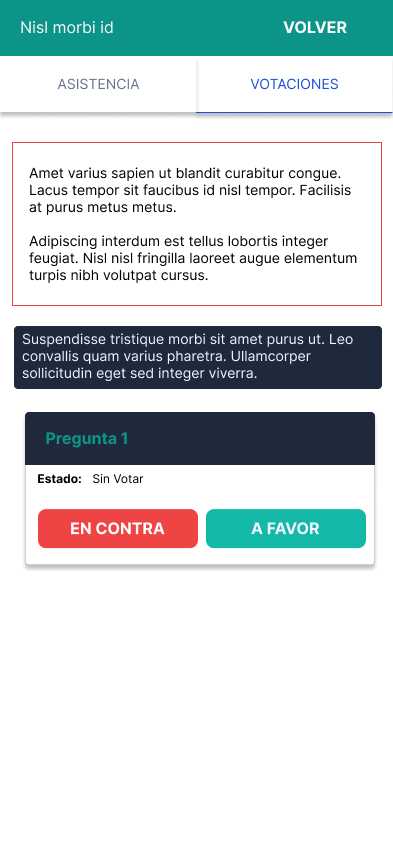
\includegraphics[width=0.3\textwidth]{resources/images/Asambleas-voto-movil}}
    \caption{Prototipo de la vista del perfil}
    \label{fig:asambleas-votacion-movil}
\end{figure}

Por último el usuario podrá visualizar su perfil en donde podrá ver su información personal además de las opciones de cierre de sesión y cambio de contraseña Figura \ref{fig:perfil-movil}.

\begin{figure}[H]
    \centering
    \fbox{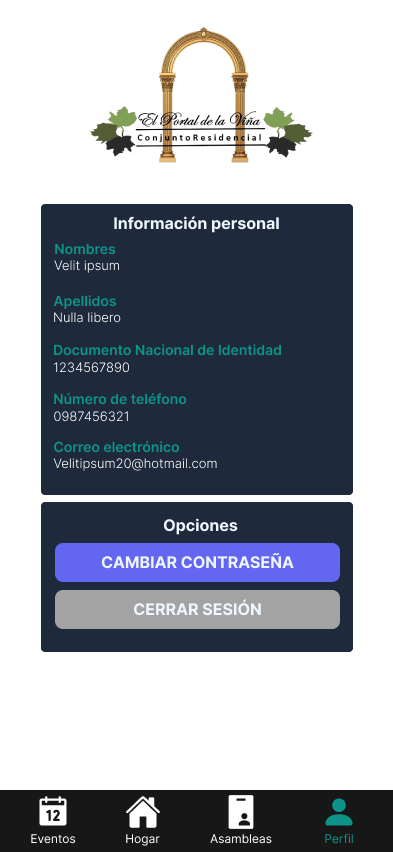
\includegraphics[width=0.3\textwidth]{resources/images/perfil-movil}}
    \caption{Prototipo de la vista del registro de voto en asambleas}
    \label{fig:perfil-movil}
\end{figure}

\subsection{Construcción}\label{subsec:construccion}
En la siguiente sección se detalla la construcción de la propuesta de los sistemas de administración de condominios, en donde se detallan los procesos que se siguieron para el desarrollo de los sistemas.
\subsubsection{Backend}

\paragraph{Dependencias de la API}

Las dependencias necesarias para el sistema de la API se utilizó Maven como gestor de dependencias.
En la Figura \ref{fig:api-dependencies} se muestra el archivo \textit{pom.xml} en donde se establecierón las dependencias necesarias para el desarrollo de la API.
El listado de todas las dependencias usadas en la API se detallan en el Anexo \ref{app:dependencias-api}.

\begin{figure}[H]
    \centering
    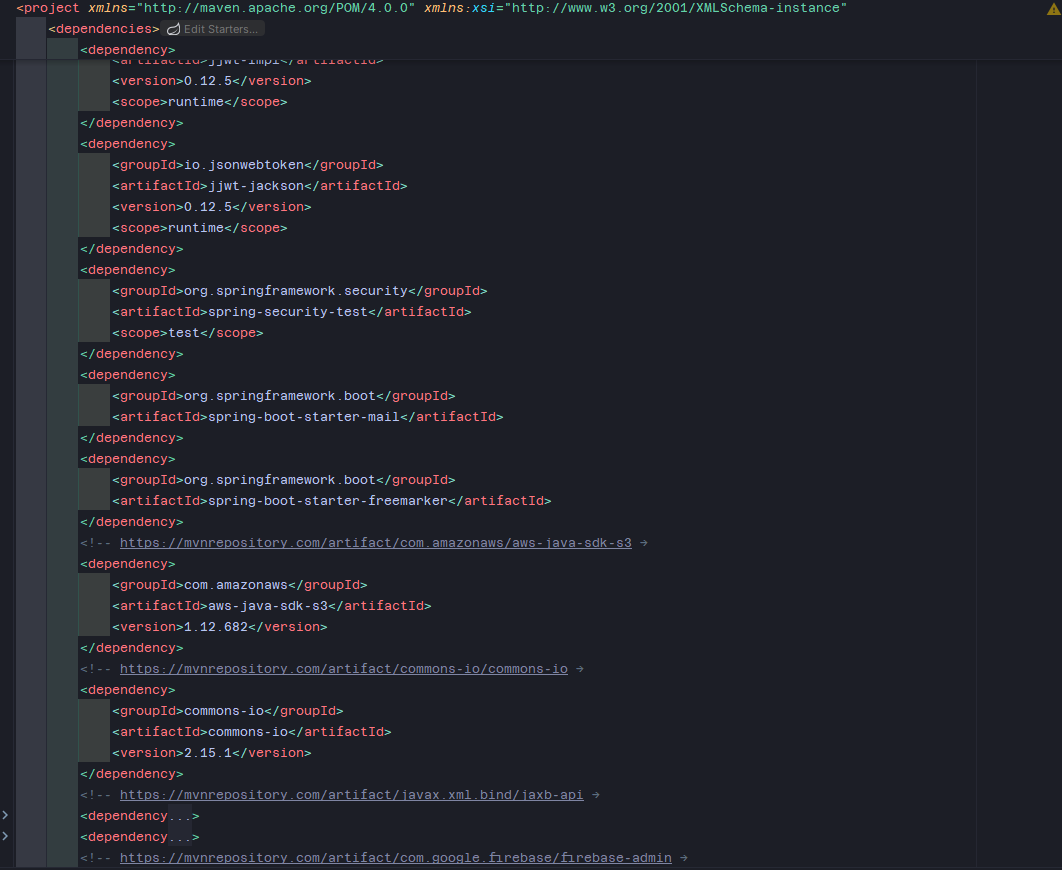
\includegraphics[width=1\textwidth]{resources/images/maven}
    \caption{Archivo \textit{pom.xml} con las dependencias Maven de la API}
    \label{fig:api-dependencies}
\end{figure}

\paragraph{Configuración de las propiedades de la API}
Para la configuración de las propiedades de la API se utilizó el archivo \textit{application.properties} en donde se establecieron las propiedades de conexión a la base de datos, el puerto en el que se ejecutará la API, la configuración del envío de mensajes via Simple Mail Transfer Protocol (SMTP), el archivo de configuración de Firebase y las variables de configuración de los servicios de almacenamiento de archivos de Amazon Web Services (AWS) Amazon Simple Storage Service (S3) como se muestra en la Figura \ref{fig:api-properties}.

\begin{figure}[H]
    \centering
    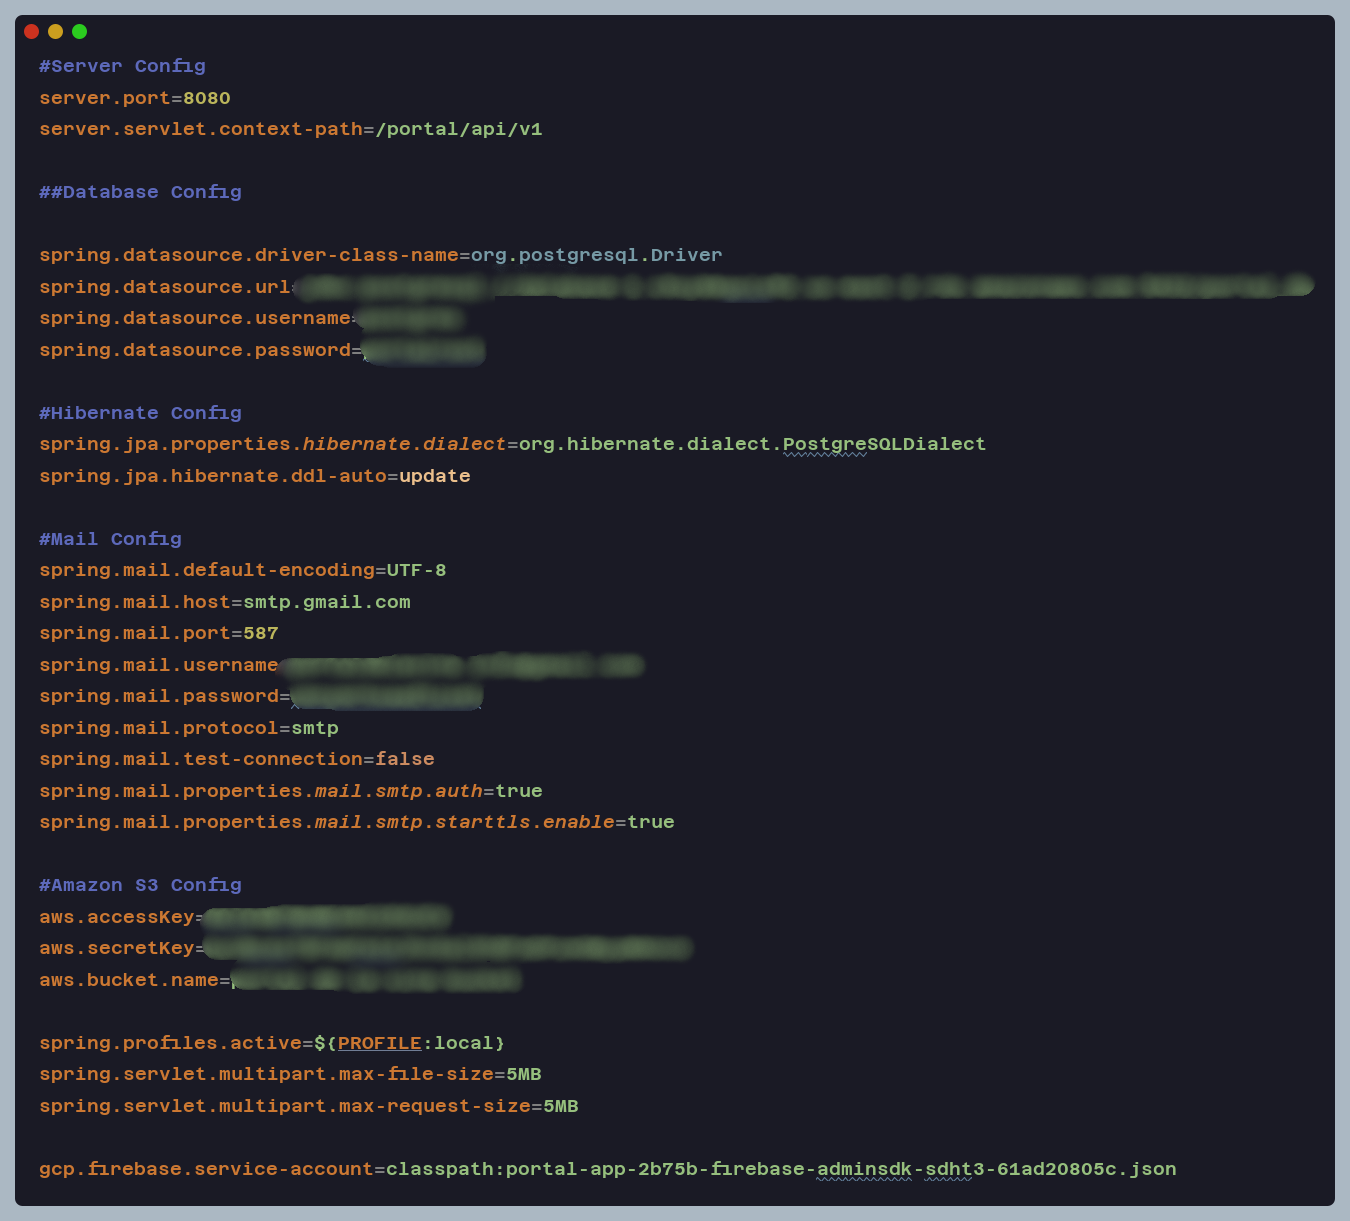
\includegraphics[width=1\textwidth]{resources/images/properties}
    \caption{Código de configuración de propiedades de la API}
    \label{fig:api-properties}
\end{figure}

\paragraph{Configuración de la seguridad de la API}

Como parte de la configuración de la seguridad de la API se utilizó Spring Security en donde se establecierón las reglas de seguridad para el acceso a los puntos de entrada expuestos en la APi mediante el uso de Json Web Token (JWT) como mecanismo de autenticación y autorización.
Adicionalmente se configurarón los Cross-Origin Resource Sharing (CORS) para permitir el acceso a la API desde la aplicación móvil y el sistema web como se muestran en la Figura \ref{fig:security}.

\begin{figure}[H]
    \centering
    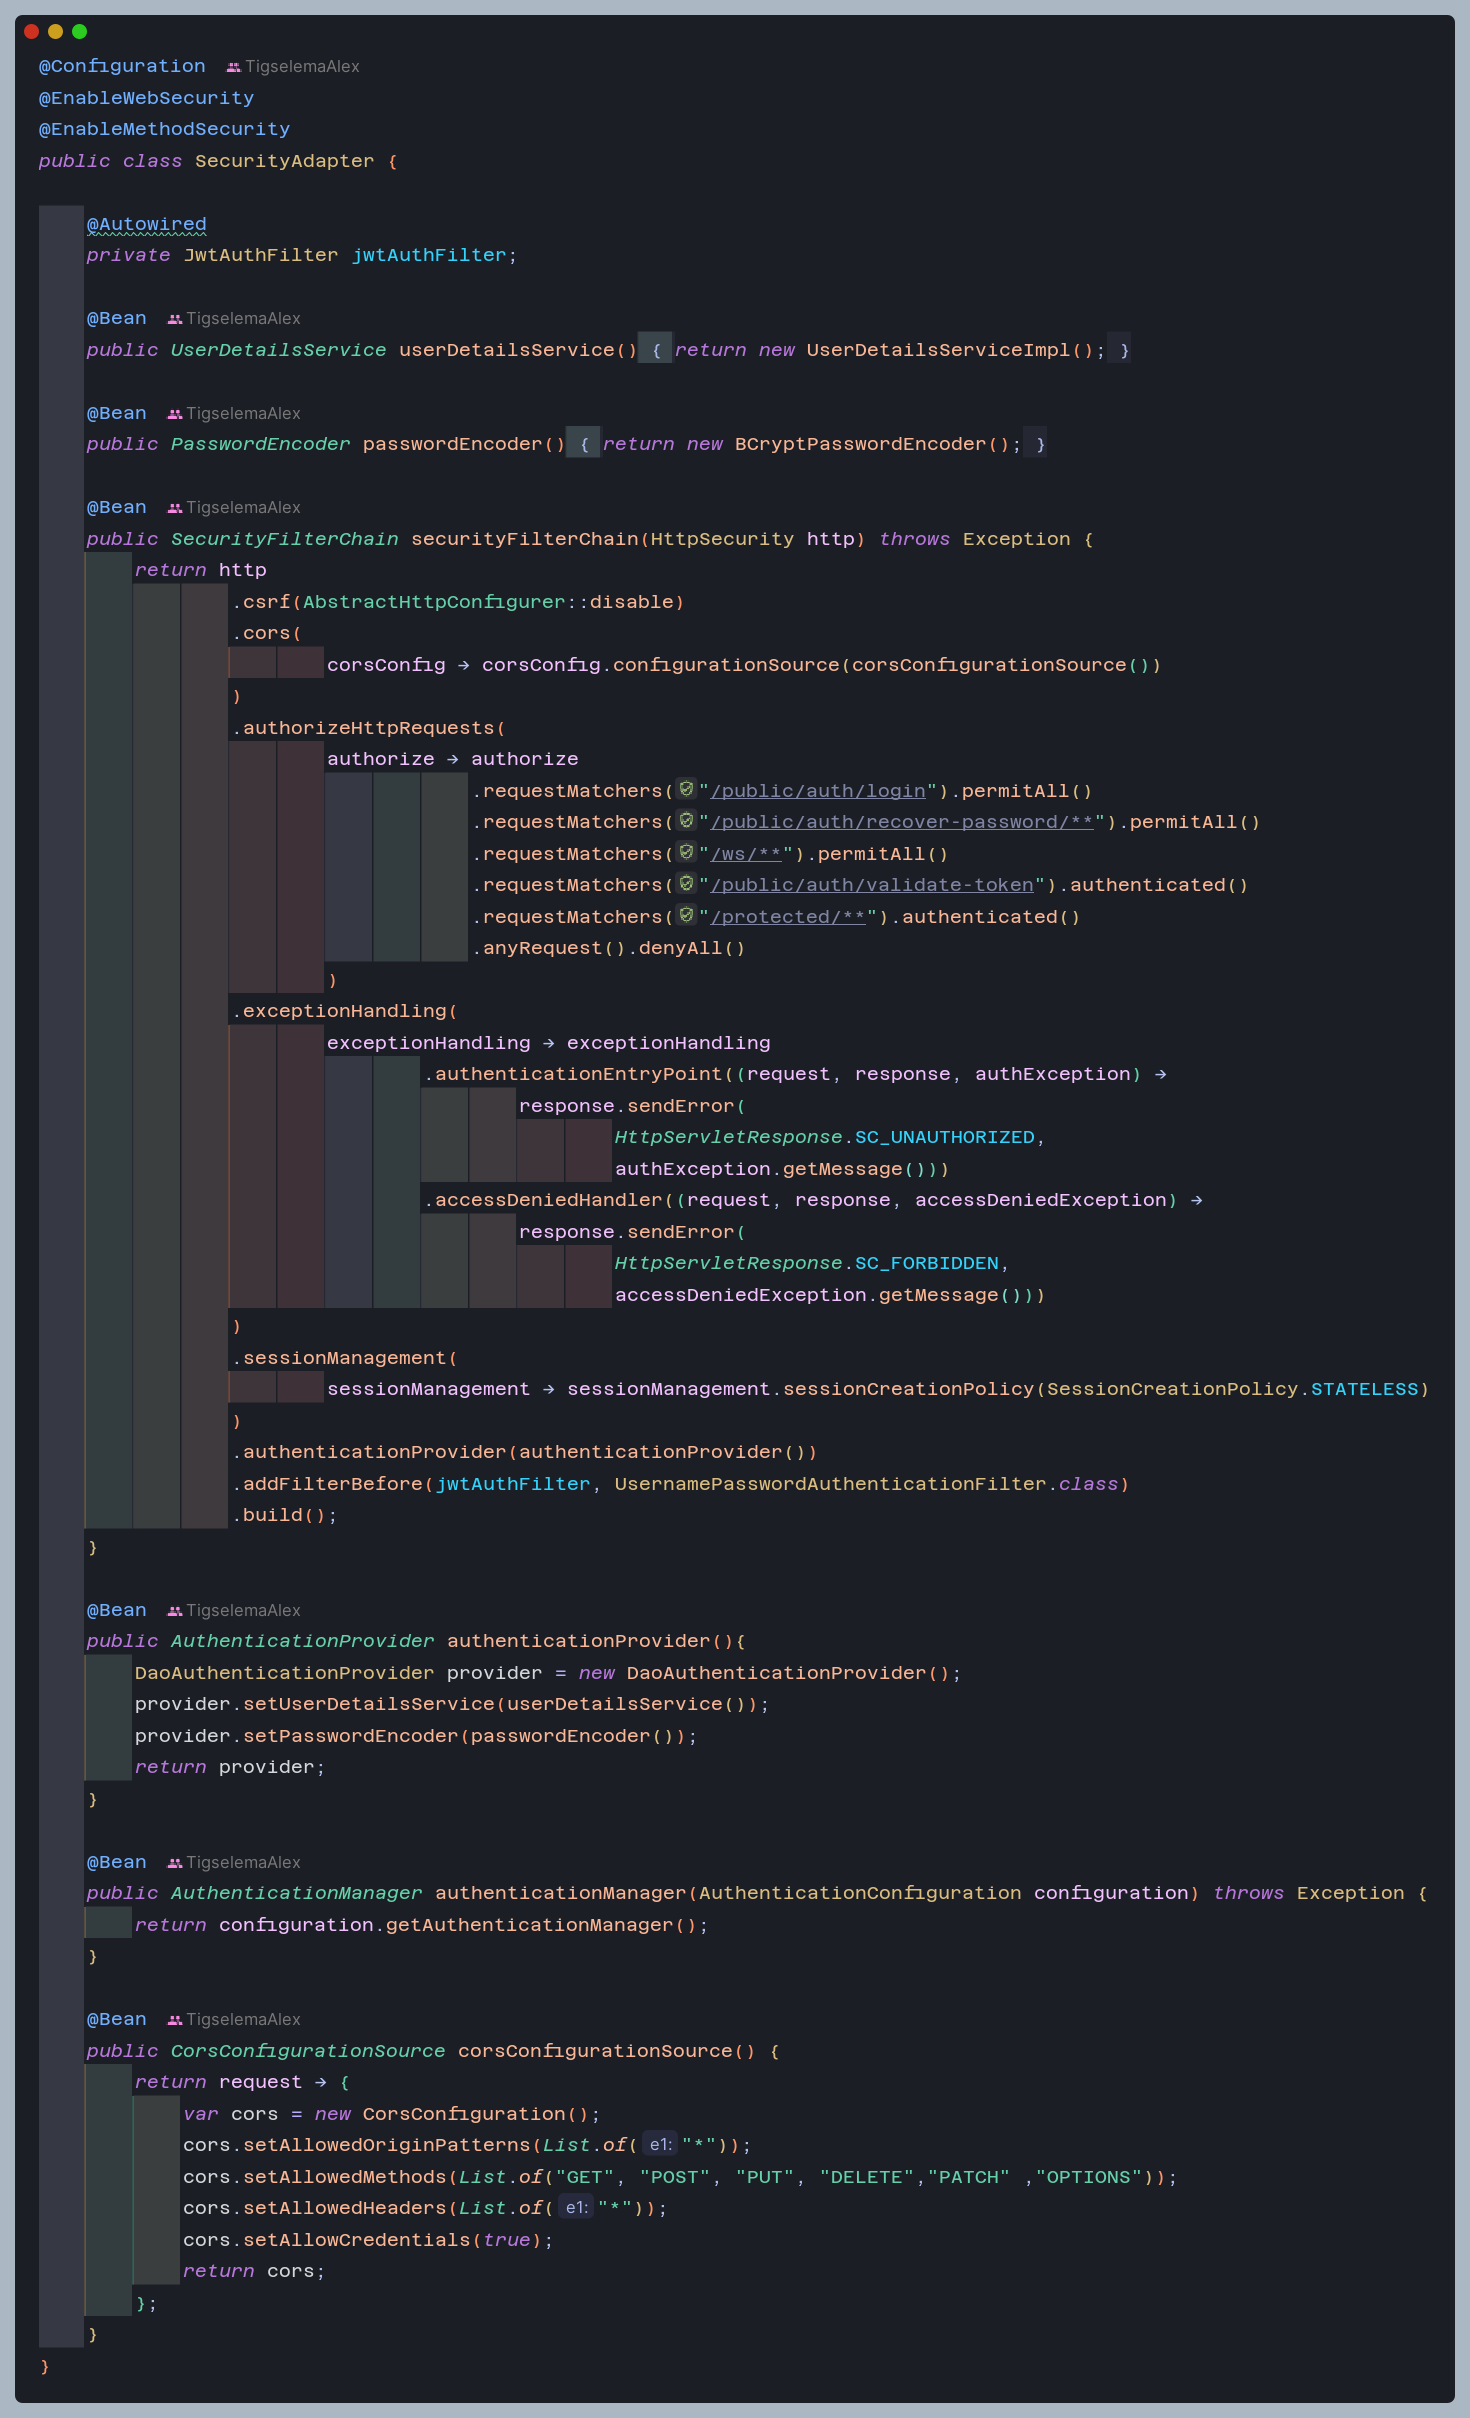
\includegraphics[width=1\textwidth]{resources/images/security}
    \caption{Código de configuración de seguridad de la API}
    \label{fig:security}
\end{figure}

\paragraph{Acceso y persistencia de datos}

Para el acceso y persistencia de datos se utilizó Spring Data JPA.
Spring Data JPA es un proyecto de Spring que facilita la creación de tablas en la base de datos y la realización de operaciones CRUD (Create, Read, Update, Delete) sobre las mismas.
Para lograr esto Spring Data JPA hace uso del mapeo objeto-relacional (ORM) de Hibernate.
\bigbreak
Para la creación de las entidades se útiliza la anotación @Entity para indicarle a Spring que esa clase será mapeada a una tabla en la base de datos.
En la Figura \ref{fig:abstract-entity} se muestra una clase abstracta AbstractEntity que contiene los atributos comunes a todas las entidades como el id, la fecha de creación, la fecha de actualización y si está activo o no.
En la Figura \ref{fig:entity} se muestra una entidad con herencia de la claseAbstractEntity, en donde se establecen los atributos y las relaciones con otras entidades para que sean mapeadas en la base de datos.

\begin{figure}[H]
    \centering
    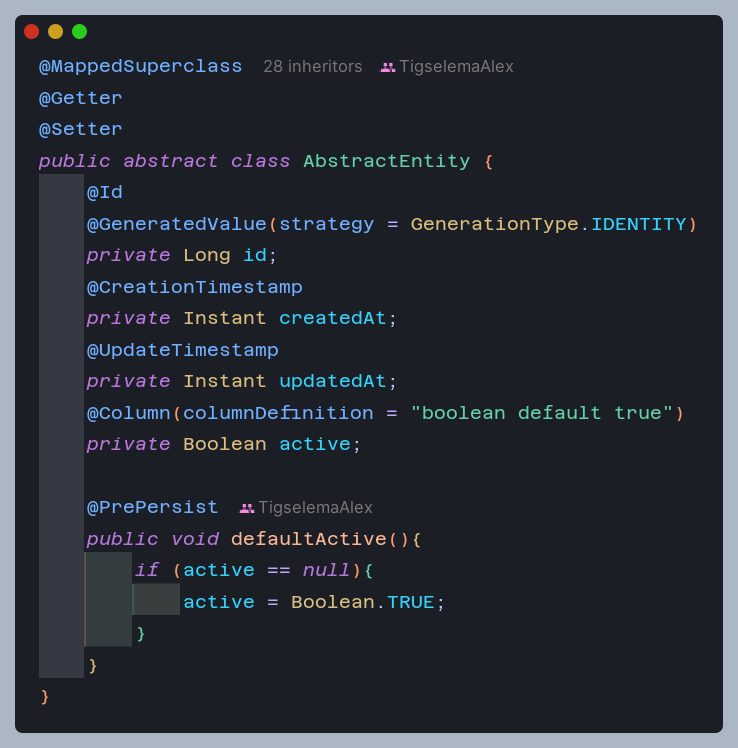
\includegraphics[width=1\textwidth]{resources/images/abstractEntity}
    \caption{Código de la clase abstracta base para las demas entidades AbstractEntity}
    \label{fig:abstract-entity}
\end{figure}

\begin{figure}[H]
    \centering
    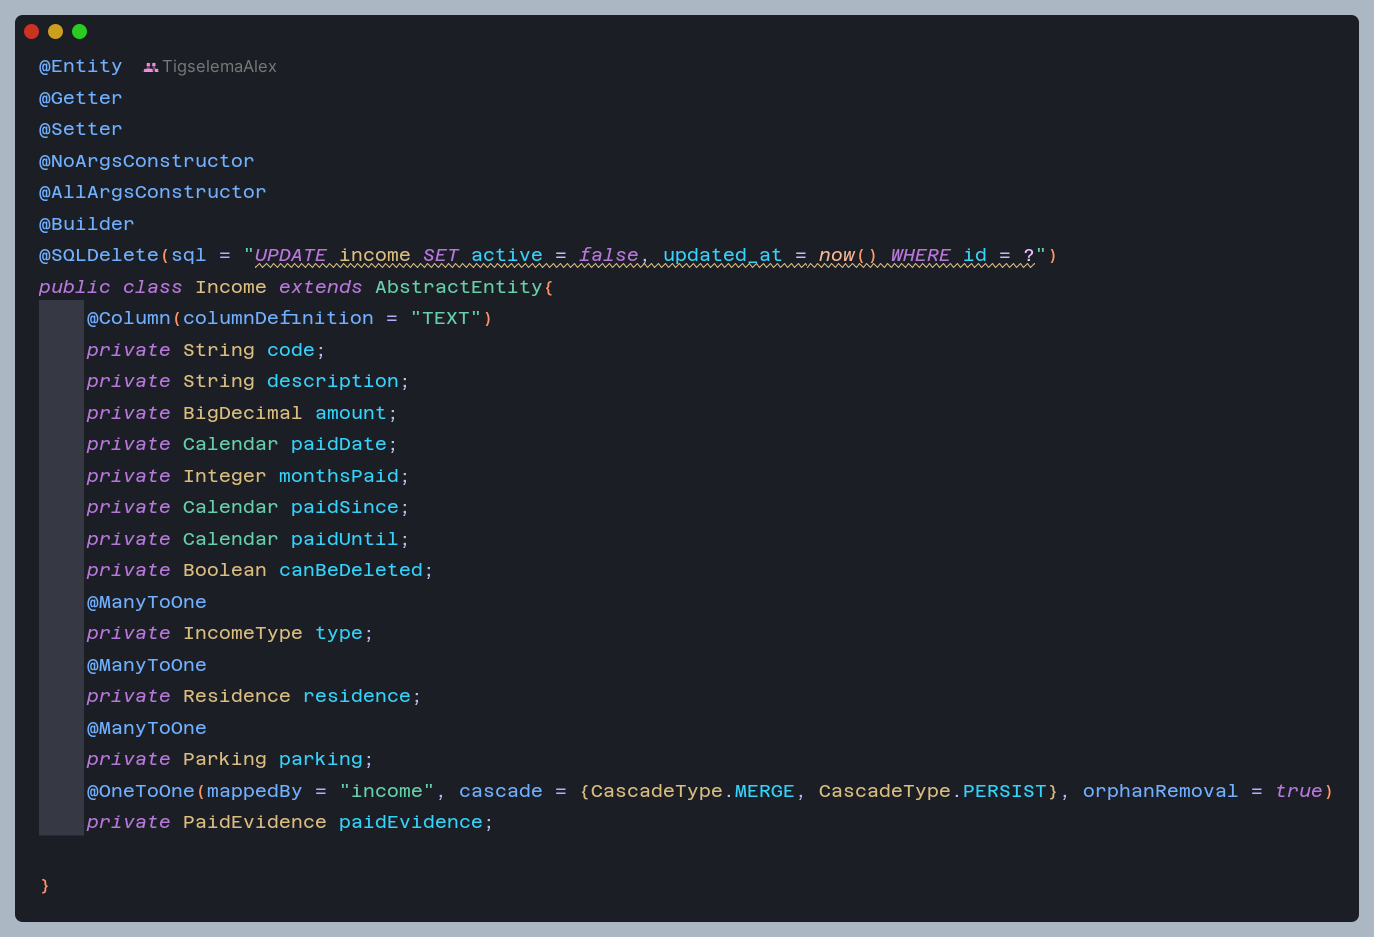
\includegraphics[width=1\textwidth]{resources/images/entity}
    \caption{Código de la entidad Income}
    \label{fig:entity}
\end{figure}

Para los procesos CRUD se utilizaron repositorios que extienden de la interfaz JpaRepository de Spring Data  tal como se muestra en la Figura \ref{fig:repository}, en donde se definen los métodos necesarios para realizar las operaciones de creación, lectura, actualización y eliminación de los registros en la base de datos además de los métodos personalizados que sean necesarios.

\begin{figure}[H]
    \centering
    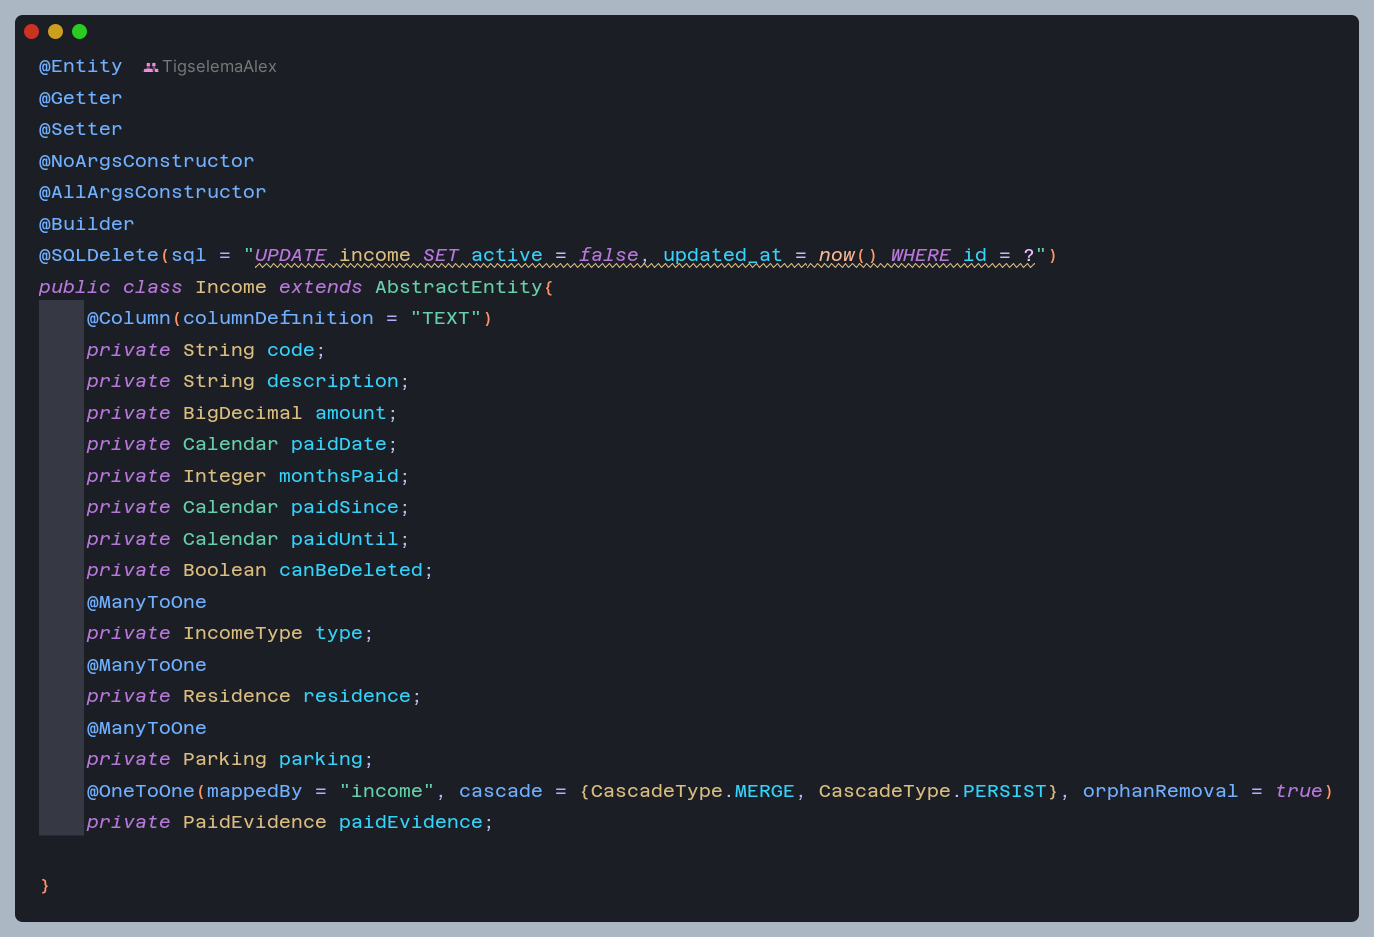
\includegraphics[width=1\textwidth]{resources/images/entity}
    \caption{Código de el repositorio para para entidad Income}
    \label{fig:repository}
\end{figure}
Posteriormente a la creación de todas las entidades se generó el siguiente diagrama entidad-relación como se muestra en las Figuras \ref{fig:er-diagram-1} y \ref{fig:er-diagram-2}.

    \begin{figure}[H]
        \centering
        \includegraphics[width=1\textwidth]{resources/images/diagram-1}
        \caption{Diagrama entidad-relación de la base de datos (Parte 1)}
        \label{fig:er-diagram-1}
    \end{figure}

\begin{figure}[H]
    \centering
    \includegraphics[width=1\textwidth]{resources/images/diagram-2}
    \caption{Diagrama entidad-relación de la base de datos (Parte 2)}
    \label{fig:er-diagram-2}
\end{figure}

\newpage

\paragraph{Configuración y uso del almacenamiento de archivos en S3}

Para poder usar los servicios de almacenamiento de AWS S3 se creo una componente o bean de configuración en donde se establecieron las credenciales de acceso al usuario de AWS y la región en donde se encuentra alojado el bucket de almacenamiento de archivos como se muestra en la Figura \ref{fig:s3-config}.

\begin{figure}[H]
    \centering
    \includegraphics[width=1\textwidth]{resources/images/s3}
    \caption{Código de configuración del almacenamiento de archivos en S3}
    \label{fig:s3-config}
\end{figure}

Para poder realizar la carga y eliminación de archivos en el bucket de almacenamiento como se ve en la Figura \ref{fig:s3-fileService}, se creó un servicio en donde se establecieron los métodos de carga en donde se reciben como parámetros el código y el archivo a cargar, en este método se genera un nombre único para el archivo y se procede a crear una petición de carga al bucket a través del método putObject de la instancia del bean inyectado AmazonS3.
Por otro lado el método de eliminación recibe como parámetro el nombre del archivo a eliminar y se procede a realizar la eliminación a través del bean inyectado AmazonS3.

\begin{figure}[H]
    \centering
    \includegraphics[width=1\textwidth]{resources/images/fileService}
    \caption{Código del servicio de carga y eliminación del archivo S3}
    \label{fig:s3-fileService}
\end{figure}


\paragraph{Configuración del motor de plantillas HTML FreeMarker y envío de correos electrónicos}

Se debe crear un componente o bean para configurar el creador de plantillas HTML para los correos electrónicos en este caso usando FreeMarker como motor de plantillas tal como se muestra en la Figura \ref{fig:freemaker}.

\begin{figure}[H]
    \centering
    \includegraphics[width=1\textwidth]{resources/images/fremaker}
    \caption{Código de configuración del motor de plantillas HTML para los correos electrónicos}
    \label{fig:freemaker}
\end{figure}

Para el envío de correos electrónicos se creo un servicio en el cual se establecen los métodos necesarios para los envíos de correos.
Se necesita crear un modelo para que éste sea mapeado en la plantilla HTML de FreeMarker, en la Figura \ref{fig:mail-service-model} se muestra un ejemplo de modelo y en la Figura \ref{fig:mail-service-method} se muestra el uso de éste modelo en un método y el envío de un correo electrónico a un usuario en particular.

\begin{figure}[H]
    \centering
    \includegraphics[width=1\textwidth]{resources/images/fremaker}
    \caption{Código de modelo para mapearlo en la plantilla HTML}
    \label{fig:mail-service-model}
\end{figure}

\begin{figure}[H]
    \centering
    \includegraphics[width=1\textwidth]{resources/images/fremaker}
    \caption{Código del método de envio de correo electrónico para recuperar la contraseña}
    \label{fig:mail-service-method}
\end{figure}

\paragraph{Configuración de Firebase para el envío de Notificaciones Push y servicio de envió de notificaciones}

Para poder enviar notificaciones push a los dispositivos móviles se debe configurar Firebase Cloud Messaging (FCM) en la API, para ello se debe crear un componente o bean de configuración en donde se establecerán las credenciales de acceso a Firebase como se muestra en la Figura \ref{fig:firebase}, dichas credenciales se obtienen de un archivo Json que se descarga desde la consola de Firebase para posteriormente referenciar su ubicación en el archivo de configuración de propiedades como se mostró en la Figura \ref{fig:api-properties}.


\begin{figure}[H]
    \centering
    \includegraphics[width=1\textwidth]{resources/images/firebase}
    \caption{Código de configuración de Firebase para el envío de Notificaciones Push}
    \label{fig:firebase}
\end{figure}

En la Figura \ref{fig:pushNotification-service} se muestra como se crea un servicio para el envío de notificaciones push y como se actualiza  el token de cada dispositivos móvil en la base de datos para poder enviar notificaciones a un dispositivo en particular.

\begin{figure}[H]
    \centering
    \includegraphics[width=0.8\textwidth]{resources/images/pushNotification}
    \caption{Código del servicio de las Notificaciones Push}
    \label{fig:pushNotification-service}
\end{figure}

\paragraph{Cálculo de la distancia de Haversine}

Como parte de la funcionalidad de la geolocalización se debe calcular la distancia entre dos puntos geográficos para poder determinar posteriormente si se encuentra dentro de un radio de aceptación.
Para este cálculo se necesitan las coordenadas del punto de referencia las cuales son almacenadas en un archivo Json en el servidor, y las coordenadas del punto a calcular la distancia.
Posteriormente se aplica la formula de Haversine como se muestra en la Figura \ref{fig:haversine} y se obtiene la distancia en metros.
Por último se compara la distancia obtenida con el radio de aceptación para determinar si el punto se encuentra dentro del rango o no tal como se ve aplicada en el registro de asistencia en la asamblea en la Figura \ref{fig:asamblea-asistencia-movil}.

\begin{figure}[H]
    \centering
    \includegraphics[width=1\textwidth]{resources/images/haversine}
    \caption{Código del cálculo de la distancia de Haversine en Java}
    \label{fig:haversine}
\end{figure}

\begin{figure}[H]
    \centering
    \includegraphics[width=1\textwidth]{resources/images/attendance-geolocation}
    \caption{Código de método de registro de asistencia en la asamblea}
    \label{fig:asamblea-asistencia-movil}
\end{figure}

\paragraph{Controladores}

Para poder exponer los puntos de salida o endpoints de la aplicación se deben crear controladores en donde se establecen las rutas y los métodos que se ejecutarán según el tipo de petición que se realice y validando los roles de los usuarios que realizan la petición tal como se muestra en la Figura \ref{fig:user-controller}.

\begin{figure}[H]
    \centering
    \includegraphics[width=1\textwidth]{resources/images/userController}
    \caption{Código del controlador de usuarios}
    \label{fig:user-controller}
\end{figure}

\subsubsection{Frontend}

\textbf{Sistema web Administrativo}
\bigbreak
\paragraph{Dependencias del sistema}

Para el desarrollo del sistema web Administrativo el cual se construyó con Angular se necesito instalar dependencias mediante el gestor de paquetes npm con el comando \textit{npm install <dependencia>}.
Estas dependencias se encuentran en el archivo \textit{package.json} como se muestra en la Figura \ref{fig:package-json}.
Entre ellas se encuentran PrimeNg, PrimeFlex, PrimeIcons, quill, chart.js, ngx-print, entre otros.

\begin{figure}[H]
    \centering
    \includegraphics[width=1\textwidth]{resources/images/dependencias-angular}
    \caption{Archivo \textit{package.json} con las dependencias del sistema web}
    \label{fig:package-json}
\end{figure}

\paragraph{Configuración de la aplicación}

Angular nos provee un archivo principal llamado \textit{app.config.ts} en donde se establecen los proveedores de servicios tales como el servicio de animaciones, el de rutas, el servicio para realizar peticiones HTTP, el servicio de localización y el servicio de optimización de imágenes como se muestra en la Figura \ref{fig:app-config}.

\begin{figure}[H]
    \centering
    \includegraphics[width=1\textwidth]{resources/images/app-config}
    \caption{Archivo \textit{app.config.ts} con la configuración de la aplicación}
    \label{fig:app-config}
\end{figure}

Adicionalmente es necesario configurar las rutas de la aplicación en el archivo \textit{app-routes.ts} en donde se establecen las rutas de los componentes que se mostrarán en la aplicación como se muestra en la Figura \ref{fig:app-routing}.

\begin{figure}[H]
    \centering
    \includegraphics[width=1\textwidth]{resources/images/app-routes}
    \caption{Archivo \textit{app-routes.ts} con la configuración de las rutas de la aplicación}
    \label{fig:app-routing}
\end{figure}

\paragraph{Inicio de sesión}

En la Figura \ref{fig:sw-login-code} se muestra el código del login en donde se tomarán las credenciales del formulario de inicio de sesión y se enviarán al servicio de autenticación para que éste realize la solicitud a la API y así el controlador de autenticación pueda validar las credenciales a través del método de autenticación definido Figura \ref{fig:api-auth-login-usecase} en donde se válidan las credenciales y en el caso de ser válidas se generará un token JWT que será enviado al cliente web para que este lo almacene en el sesión storage y pueda ser utilizado en las demás peticiones mediante el interceptador de peticiones HTTP definido en el sistema web Figura \ref{fig:sw-interceptor}.

\begin{figure}[H]
    \centering
    \includegraphics[width=1\textwidth]{resources/images/sw-login-code}
    \caption{Código del inicio de sesión en el frontend}
    \label{fig:sw-login-code}
\end{figure}

\begin{figure}[H]
    \centering
    \includegraphics[width=1\textwidth]{resources/images/api-auth-login-usecase}
    \caption{Código del método de autenticación en el API}
    \label{fig:api-auth-login-usecase}
\end{figure}

\begin{figure}[H]
    \centering
    \includegraphics[width=1\textwidth]{resources/images/sw-login}
    \caption{Página de inicio de sesión}
    \label{fig:sw-login-page}
\end{figure}

\begin{figure}[H]
    \centering
    \includegraphics[width=1\textwidth]{resources/images/sw-interceptor}
    \caption{Código del interceptor de peticiones HTTP en el sistema web}
    \label{fig:sw-interceptor}
\end{figure}

\paragraph{Gestión de usuarios}

Los usuarios del condominio únicamente podrán ser registrado por el administrador para lo cual se debe ingresar los datos personales proporcionados por el usuario y se debe seleccionar el rol que tendrá el usuario dentro del condominio.
Ésta información será enviada a la API en un cuerpo de tipo JSON para que ésta pueda ser procesada y almacenada en la base de datos.
Una vez registrado el usuario podrá ser visualizado en la tabla de usuarios en donde se podrá editar o eliminar el usuario tal como se muestra en la Figura \ref{fig:sw-usuarios}.

\begin{figure}[H]
    \centering
    \includegraphics[width=1\textwidth]{resources/images/api-controller-findall}
    \caption{Endpoint para obtener todos los usuarios}
    \label{fig:api-findAll-controller}
\end{figure}

\begin{figure}[H]
    \centering
    \includegraphics[width=1\textwidth]{resources/images/sw-usuarios}
    \caption{Página de gestión de usuarios}
    \label{fig:sw-usuarios}
\end{figure}

\begin{figure}[H]
    \centering
    \includegraphics[width=1\textwidth]{resources/images/api-crotroller-create-user}
    \caption{Endpoint para crear un usuario}
    \label{fig:api-controller-create-user}
\end{figure}

\begin{figure}[H]
    \centering
    \includegraphics[width=1\textwidth]{resources/images/sw-usuarios-form}
    \caption{Formulario de creación y edición de usuarios}
    \label{fig:sw-create-user-form}
\end{figure}


\paragraph{Gestión de geolocalización}

El usuario administrador podrá actualizar el punto de referencia para la geolocalización de la asamblea en donde se podrá visualizar un mapa con la ubicación actual y una circunferencia representado el radio de aceptación.
Para la modificación de éste punto de referencia se debe enviar la latitud, la longitud y el radio de aceptación en un cuerpo de tipo JSON a la API en donde se procesara ésta información leyendo el archivo JSON del servidor y modificando sus valores tal como se muestra en la Figura \ref{fig:api-geolocation-update}.


\begin{figure}[H]
    \centering
    \includegraphics[width=1\textwidth]{resources/images/api-geolocation-update-method}
    \caption{Método de actualización de la geolocalización en el API}
    \label{fig:api-geolocation-update}
\end{figure}

\begin{figure}[H]
    \centering
    \includegraphics[width=1\textwidth]{resources/images/sw-geolocation}
    \caption{Página de gestión de geolocalización}
    \label{fig:sw-geolocation}
\end{figure}

\paragraph{Gestión de residencias}

El presidente o vicepresidente podrá registrar en las residencias el usuario representante de la misma para ello se debe enviar a la API el id del usuario representante y el id de la residencia en un cuerpo de tipo JSON.
La API procesará esta información y actualizará el usuario representante de la residencia tal como se muestra en la Figura \ref{fig:api-residence-update}.

\begin{figure}[H]
    \centering
    \includegraphics[width=1\textwidth]{resources/images/api-update-residence-endpoint}
    \caption{Endpoint para actualizar el usuario representante de una residencia}
    \label{fig:api-residence-update}
\end{figure}

\begin{figure}[H]
    \centering
    \includegraphics[width=1\textwidth]{resources/images/sw-residente-update}
    \caption{Formulario de actualización de usuario representante de una residencia}
    \label{fig:sw-residente-update}
\end{figure}

\paragraph{Gestión de parqueaderos}

Como parte de la gestión de parqueaderos el presidente visualizará un mapa con la ubicación de los parqueaderos en grupos de dos colores en donde los azules representan a los de zona azul y los amarillos a los partículares.
Para poder la casa asociada a un parqueadero se debe seleccionar el parqueadero de uno de los grupos y seleccionar la casa a la que se le desea asignar el parqueadero, de esta manera se enviarán a la API el id de la casa y el id del parqueadero.
La API procesará la solicitud y actualizará la casa asociada a ese parqueadero tal como se muestra en la Figura \ref{fig:api-parking-update}.

\begin{figure}[H]
    \centering
    \includegraphics[width=1\textwidth]{resources/images/api-parking-update-method}
    \caption{Método de actualización de la casa asociada a un parqueadero en la API}
    \label{fig:api-parking-update}
\end{figure}

\begin{figure}[H]
    \centering
    \includegraphics[width=1\textwidth]{resources/images/sw-parking-group}
    \caption{Página de gestión de parqueaderos}
    \label{fig:sw-parking-group}
\end{figure}

\begin{figure}[H]
\centering
\includegraphics[width=1\textwidth]{resources/images/sw-parking-form}
\caption{Formulario de actualización de la casa asociada a un parqueadero}
\label{fig:sw-parking-form}
\end{figure}

\paragraph{Gestión de incidentes}

El control de los incidentes reportados por los guardías serán gestionados por el presidente y vicepresidente los cuales se deberá de proporcionar la información reportada por el guardía y en el caso de ser necesario subir evidencias del incidente.
Para ello se debe enviar el id del guardía que reportó el incidente, el asunto de incidente, una descripción, el tipo de incidente y las evidencias en formato form-data a la API tal como se muestra en la Figura \ref{fig:api-incident-create}.
Estos incidentes registrados podrán ser actualizados en el caso de que se lleguen a solucionar o queden inconclusos para poder generar un reporte del incidente tal como se muestra en la Figura \ref{fig:sw-guard-incidents-report}.

\begin{figure}[H]
    \centering
    \includegraphics[width=1\textwidth]{resources/images/api-guard-indicent-endpoint}
    \caption{Endpoint para crear un incidente}
    \label{fig:api-incident-create}
\end{figure}

\begin{figure}[H]
    \centering
    \includegraphics[width=1\textwidth]{resources/images/sw-guard-incidents}
    \caption{Página de gestión de incidentes}
    \label{fig:sw-guard-incidents}
\end{figure}

\begin{figure}[H]
    \centering
    \includegraphics[width=1\textwidth]{resources/images/sw-guard-incidents-form}
    \caption{Formulario de creación y edición de incidentes}
    \label{fig:sw-guard-incident-form}
\end{figure}

\begin{figure}[H]
    \centering
    \includegraphics[width=1\textwidth]{resources/images/sw-guard-incidents-report}
    \caption{Reporte de incidente}
    \label{fig:sw-guard-incidents-report}
\end{figure}

\paragraph{Gestión de convocatorias}

Para el registro de convocatorias se debe establecer la fecha de inicio, de que tipo de convocatoria es ya que dependiendo de si es una asamblea se podrá establecer la fecha y hora límite para el registro de asistencia por parte de los residentes mediante el uso de la aplicación móvil, el asunto de la convocatoria y una descripción a cerca de los temas o actividades a tratar en la convocatoria.
Esta información será enviada a la API en formato JSON para que ésta pueda ser registrada y notificar a los demás residentes solo en el caso de ser una asamblea tal como se muestra en la Figura \ref{fig:api-convocation-create}.
Adicionalmente se puede visualizar la convocatoria para ser descargada en formato PDF para poder ser compartida en los grupos de WhatsApp tal como se muestra en la Figura \ref{fig:sw-convocatorias-comunicado}.


\begin{figure}[H]
    \centering
    \includegraphics[width=1\textwidth]{resources/images/api-convocation-create-usecase}
    \caption{Método de creación de una convocatoria y envio de notificación push en la API}
    \label{fig:api-convocation-create}
\end{figure}

\begin{figure}[H]
    \centering
    \includegraphics[width=1\textwidth]{resources/images/sw-convocatorias}
    \caption{Página de gestión de convocatorias}
    \label{fig:sw-convocatorias}
\end{figure}

\begin{figure}[H]
    \centering
    \includegraphics[width=1\textwidth]{resources/images/sw-convocatorias-form}
    \caption{Formulario de creación y edición de convocatorias}
    \label{fig:sw-convocatorias-formulario}
\end{figure}

\begin{figure}[H]
    \centering
    \includegraphics[width=1\textwidth]{resources/images/sw-convocatorias-comunicado}
    \caption{Vista previa a la descarga del comunidado de la convocatoria en PDF}
    \label{fig:sw-convocatorias-comunicado}
\end{figure}

\paragraph{Gestión de asistencias en asambleas}

Para las convocatorias que son asambleas tendrán habilitada la opción de poder administrar las asistencias, en donde se listarán todas las residencias junto con la información de los residentes asociados a cada una de ellas.
Para el registro de asistencia manual se selecciona la casa y se coloca su estado de asistencia y en el caso de ser necesario se puede registrar el nombre de la persona que asiste representando esa residencia sin ser la persona asociada a ella.
A la API se le envía el id de la convocatoria, el id de la residencia, el estado de la asistencia y opcionalmente el nombre de la persona que asiste tal como se muestra en la Figura \ref{fig:api-attendance-create}.
Adicionalmente se puede obtener un reporte de las casas ausentes para poder realizar su descarga e informar a los residentes por los grupos de comunicación tal como se muestra en la Figura \ref{fig:sw-asamblea-asistencia-reporte}.

\begin{figure}[H]
    \centering
    \includegraphics[width=1\textwidth]{resources/images/api-asamblea-asistencia-manual}
    \caption{Método del registro de asistencia manual en la API}
    \label{fig:api-attendance-create}
\end{figure}

\begin{figure}[H]
    \centering
    \includegraphics[width=1\textwidth]{resources/images/sw-asamblea-asistencia}
    \caption{Página de gestión de asistencia en asambleas}
    \label{fig:sw-asamblea-asistencia}
\end{figure}

\begin{figure}[H]
    \centering
    \includegraphics[width=1\textwidth]{resources/images/sw-asamblea-asistencia-reporte}
    \caption{Reporte de inasistencias en la asamblea}
    \label{fig:sw-asamblea-asistencia-reporte}
\end{figure}

\paragraph{Gestión de votación en asambleas}

Para las convocatorias que son asambleas se pueden registrar preguntas para que sean votadas por los residentes, en donde se registrará las preguntas para lo cual solo es necesario proporcionar el enunciado de la pregunta y enviarla a la API en formato JSON como se muestra en la Figura \ref{fig:api-question-create}.
Una vez registrada la pregunta se debe habilitar para que los residentes puedan realizar la votación a través de la aplicación móvil, adicionalmente se podrán ver más detalladamente los votos de cada pregunta \ref{fig:sw-asamblea-votaciones-detail}, para lo cual se le debe enviar a la API el id de la pregunta por la ruta tal como se muestra en la Figura \ref{fig:api-question-toggle}.

\begin{figure}[H]
    \centering
    \includegraphics[width=1\textwidth]{resources/images/api-pregunta-crear}
    \caption{Endpoint para crear una pregunta de asamblea}
    \label{fig:api-question-create}
\end{figure}

\begin{figure}[H]
    \centering
    \includegraphics[width=1\textwidth]{resources/images/api-pregunta-listar-todos}
    \caption{Endpoint para obtener todas las preguntas de asamblea}
    \label{fig:api-question-all}
\end{figure}

\begin{figure}[H]
    \centering
    \includegraphics[width=1\textwidth]{resources/images/api-pregunta-toggle}
    \caption{Endpoint para habilitar o deshabilitar una pregunta de asamblea}
    \label{fig:api-question-toggle}
\end{figure}

\begin{figure}[H]
    \centering
    \includegraphics[width=1\textwidth]{resources/images/sw-asamblea-votaciones}
    \caption{Lista de preguntas de asamblea}
    \label{fig:sw-asamblea-votaciones}
\end{figure}

\begin{figure}[H]
    \centering
    \includegraphics[width=1\textwidth]{resources/images/sw-asamblea-votaciones-detalle}
    \caption{Listado detallado de votaciones de una pregunta de asamblea}
    \label{fig:sw-asamblea-votaciones-detail}
\end{figure}

\paragraph{Gestión de ingresos mensuales}

Para el registro de un ingreso mensual se debe proporcionar el o los meses de abono, la residencia a la que se le registra el pago junto con un comprobante de pago en formato de imagen, la fecha del pago y el monto se calcula automáticamente según el tipo de pago mensual tal y como se muestra en la Figura \ref{fig:sw-tesoreria-mensual-form}.
Esta información será enviada a la API en formato form-data para que ésta pueda ser procesada y almacenada en la base de datos tal como se muestra en la Figura \ref{fig:api-tesoreria-mensual-save}.

\begin{figure}[H]
    \centering
    \includegraphics[width=1\textwidth]{resources/images/sw-tesoreria-mensual-listar}
    \caption{Listado de los ingresos de tipo mensual}
    \label{fig:sw-tesoreria-mensual-listar}
\end{figure}

\begin{figure}[H]
    \centering
    \includegraphics[width=1\textwidth]{resources/images/api-listar-mensuales}
    \caption{Endpoint para listar los ingresos mensuales}
    \label{fig:api-tesoreria-mensual-listar}
\end{figure}

\begin{figure}[H]
    \centering
    \includegraphics[width=1\textwidth]{resources/images/sw-tesoreria-mensual-form}
    \caption{Formulario de creación y edición de ingresos mensuales}
    \label{fig:sw-tesoreria-mensual-form}
\end{figure}

\begin{figure}[H]
    \centering
    \includegraphics[width=1\textwidth]{resources/images/api-mensual-save}
    \caption{Endpoint para guardar un ingreso mensual}
    \label{fig:api-tesoreria-mensual-save}
\end{figure}


\paragraph{Gestión de multas}

Para el registro de multas se realiza un proceso similar al de los ingresos mensuales, salvo por la diferencia que este pago no tiene meses de abono ya que es un pago único, se debe proporcionar la residencia a que se le registra la multa, la cual puede estar o no pagada, junto con su comprobante en el caso de ser pagad, y adicionalmente se pueden adjuntar evidencias tal y como se muestra en la Figura \ref{fig:sw-tesoreria-multa-form}.
Esta información será enviada a la API en formato form-data para que ésta pueda ser procesada y almacenada en la base de datos.


\begin{figure}[H]
    \centering
    \includegraphics[width=1\textwidth]{resources/images/sw-tesoreria-multas-listar}
    \caption{Listado de multas}
    \label{fig:sw-tesoreria-multa-listar}
\end{figure}

\begin{figure}[H]
    \centering
    \includegraphics[width=1\textwidth]{resources/images/api-multas-listar}
    \caption{Endpoint para listar las multas}
    \label{fig:api-tesoreria-multa'listar}
\end{figure}

\begin{figure}[H]
    \centering
    \includegraphics[width=1\textwidth]{resources/images/sw-tesoreria-multas-form}
    \caption{Formulario de creación y edición de multas}
    \label{fig:sw-tesoreria-multa-form}
\end{figure}



\paragraph{Gestión de egresos}

El registro de egresos se realizan proporcionando el concepto del egreso, la fecha en la que se realizó el egreso, el monto del egreso y el comprobante de pago en formato de imagen o en formato PDF, junto con el proveedor del servicio o producto adquirido y el tipo de egreso tal y como se muestra en la Figura \ref{fig:sw-tesoreria-egreso-form}.
La información es enviado a la API en formato form-data para que ésta pueda ser procesada y almacenada en la base de datos tal como se muestra en la Figura \ref{fig:api-tesoreria-egreso-save}.

\begin{figure}[H]
    \centering
    \includegraphics[width=1\textwidth]{resources/images/sw-tesoreria-egresos-listar}
    \caption{Listado de los egresos}
    \label{fig:sw-tesoreria-egreso-listar}
\end{figure}

\begin{figure}[H]
    \centering
    \includegraphics[width=1\textwidth]{resources/images/api-egreso-listar}
    \caption{Endpoint para listar los egresos}
    \label{fig:api-tesoreria-egresos-listar}
\end{figure}

\begin{figure}[H]
    \centering
    \includegraphics[width=1\textwidth]{resources/images/sw-tesoreria-egresos-form}
    \caption{Formulario de creación y edición de egresos}
    \label{fig:sw-tesoreria-egreso-form}
\end{figure}

\begin{figure}[H]
    \centering
    \includegraphics[width=1\textwidth]{resources/images/api-egreso-save}
    \caption{Endpoint para guardar un ingreso mensual}
    \label{fig:api-tesoreria-egreso-save}
\end{figure}

\textbf{Aplicación Móvil}
\bigbreak
\paragraph{Dependencias de la aplicación}

Para desarrollar la aplicación móvil se utilizarón algunas dependencias extras de Capacitor como lo son el plugin de geolocalización, el plugin de notificaciones push y el plugin de dispositivos para poder obtener la información del dispositivo en donde se instala la aplicación como se pueden observar en la Figura \ref{fig:app-dependencias}.
También se utilizó TailwindCss como librería de estilos para el diseño de la aplicación.
\begin{figure}[H]
    \centering
    \includegraphics[width=0.8\textwidth]{resources/images/app-dependencias}
    \caption{Dependencias de la applicación móvil hecha con Ionic}
    \label{fig:app-dependencias}
\end{figure}

\paragraph{Configuración de la aplicación}

Se debe configurar la aplicación móvil para que se puedan realizar las peticiones a la API, para ello se debe establecer la URL de la API en el archivo \textit{environment.ts} como se muestra en la Figura \ref{fig:app-environment}, y adicionalmente configurar el archivo \textit{main.ts} para colocar los proveedores de peticiones HTTP, el proveedor de enrutamiento y los servicios de almacenamiento.

\begin{figure}[H]
    \centering
    \includegraphics[width=1\textwidth]{resources/images/app-env}
    \caption{Configuración de la URL de la API en la aplicación móvil}
    \label{fig:app-environment}
\end{figure}

\begin{figure}[H]
    \centering
    \includegraphics[width=1\textwidth]{resources/images/app-main}
    \caption{Codigo del archivo de configuración principal de la aplicación móvil}
    \label{fig:app-main}
\end{figure}

También es importante configurar Firebase para el envío de Notificaciones Push al dispositivo, para ello se debe crear un servicio en donde se establecerán el registro y los métodos de escucha de las notificaciones tal como se muestra en la Figura \ref{fig:app-push}.
Adicionalmente es necesario copiar el archivo JSON \textit{google.services.json} de Firebase en la carpeta \textit{android/app/src} de la aplicación móvil y agregar en el archivo \textit{variables.gradle} la referencia al plugin de Firebase como se muestra en la Figura \ref{fig:app-gradle}.

\begin{figure}[H]
    \centering
    \includegraphics[width=1\textwidth]{resources/images/app-push}
    \caption{Codigo del servicio de Notificaciones Push en la aplicación móvil}
    \label{fig:app-push}
\end{figure}

\begin{figure}[H]
    \centering
    \includegraphics[width=1\textwidth]{resources/images/app-firebase-config}
    \caption{Ubicación del archivo \textit{google.services.json}}
    \label{fig:app-firebase-config}
\end{figure}

\begin{figure}[H]
    \centering
    \includegraphics[width=1\textwidth]{resources/images/app-gradle}
    \caption{Código del archivo \textit{variables.gradle} con la referencia al plugin de Firebase}
    \label{fig:app-gradle}
\end{figure}

Finalmente en el archivo \textit{manifest.xml} se debe establecer los permisos necesarios para el uso de la geolocalización y notificaciones push como se muestra en la Figura \ref{fig:app-manifest}.

\begin{figure}[H]
    \centering
    \includegraphics[width=1\textwidth]{resources/images/app-manifest}
    \caption{Código del archivo \textit{manifest.xml} con los permisos necesarios}
    \label{fig:app-manifest}
\end{figure}

\paragraph{Inicio de sesión}

Para el inicio de sesión el usuario debe proporcionar sus credenciales las cuales serán enviadas a la API para que sean válidadas y en el caso de ser correctas generar un JWT que será almacenando de manera local en el dispositivo móvil para ser utilizado en las demás peticiones a través de un interceptor.

\begin{figure}[H]
    \centering
    \fbox{\includegraphics[width=0.3\textwidth]{resources/images/app-login}}
    \caption{Página de inicio de sesión}
    \label{fig:app-login}
\end{figure}

\paragraph{Visualizar calendario}

Los usuarios podrán visualizar los eventos próximos al dia actual y podrán ver detalladamente cada evento.
Para ello se toma la fecha actual desde la API y se evalúan todos las convocatorias que sean de tipo asamblea y esta es enviada como respuesta para obtener los eventos próximos a la fecha actual tal como se muestra en la Figura \ref{fig:api-event-filter}.

\begin{figure}[H]
    \centering
    \includegraphics[width=1\textwidth]{resources/images/api-calendar}
    \caption{Método para obtener las convocatorias próximas}
    \label{fig:api-event-filter}
\end{figure}

\begin{figure}[H]
    \centering
    \fbox{\includegraphics[width=0.3\textwidth]{resources/images/app-eventos}}
    \caption{Página de las próximas asambleas}
    \label{fig:app-events}
\end{figure}

\begin{figure}[H]
    \centering
    \fbox{\includegraphics[width=0.3\textwidth]{resources/images/app-eventos-detalle}}
    \caption{Detalle de una asamblea}
    \label{fig:app-eventos-detalle}
\end{figure}

\paragraph{Visualizar estado de las obligaciones financieras}

En la Figura \ref{fig:api-financial-obligations} se muestra el código de los endpoints de la API para obtener las obligaciones financieras de un usuario en particular, en donde se obtiene el id del usuario que ha iniciado sesión y se envía en la ruta de las peticiónes a la API y esta devuelve un conjunto de listados en las cuales se encuentran las los últimos diez pagos realizados por el usuario tanto en multas como en mensualidades, las multas sin pagar, y el estado por residencia del usuario en el cual se encuentran el pago de alícuotas y el pago de parqueaderos azules en el caso de que éste posea alguno tal como se muestra en la Figura \ref{fig:app-financial-obligations}.

\begin{figure}[H]
    \centering
    \fbox{\includegraphics[width=0.3\textwidth]{resources/images/app-mi-hogar}}
    \caption{Página de el estado de las obligaciones financieras}
    \label{fig:app-financial-obligations}
\end{figure}

\begin{figure}[H]
    \centering
    \includegraphics[width=1\textwidth]{resources/images/api-endpoints-obligaciones}
    \caption{Endpoints para obtener las obligaciones financieras de un usuario}
    \label{fig:api-financial-obligations}
\end{figure}

\begin{figure}[H]
    \centering
    \fbox{\includegraphics[width=0.3\textwidth]{resources/images/app-mi-hogar-pagos}}
    \caption{Página de los últimos pagos realizados por el usuario}
    \label{fig:app-pagos}
\end{figure}

\begin{figure}[H]
    \centering
    \fbox{\includegraphics[width=0.3\textwidth]{resources/images/app-multas-sin-pagar}}
    \caption{Página de las multas sin pagar}
    \label{fig:app-multas}
\end{figure}


\paragraph{Registrar asistencia}

Como se muestra en la Figura \ref{fig:app-asistencia-codigo} el se envía la ubicación actual del dispositivo móvil y el id del usuario que ha iniciado sesión y en un cuerpo la latitud, longitud, la residencia a la que esta registrando como asistente y un el identificador del dispositivo móvil para poder registrar la asistencia en la asamblea.
La API validará la ubicación a través del calculo de Haversine y en el caso de que la distancia sea menor al radio de aceptación se procederá a registrar la asistencia en la asamblea tal como se muestra en la Figura \ref{fig:app-asistencia}.

\begin{figure}[H]
    \centering
    \includegraphics[width=1\textwidth]{resources/images/app-asistencia-codigo}
    \caption{Código para registrar la asistencia en la asamblea}
    \label{fig:app-asistencia-codigo}
\end{figure}

\begin{figure}[H]
    \centering
    \includegraphics[width=1\textwidth]{resources/images/api-asistencia}
    \caption{Endpoint para registrar la asistencia en la asamblea}
    \label{fig:api-asistencia}
\end{figure}

\begin{figure}[H]
    \centering
    \fbox{\includegraphics[width=0.3\textwidth]{resources/images/app-asambleas-asistencias}}
    \caption{Página de asistencia en la asamblea}
    \label{fig:app-asistencia}
\end{figure}

\paragraph{Registrar voto}

Como se muestra en la Figura \ref{fig:api-votacion-codigo}, el registro del voto se realiza enviando el id del usuario, el id de la pregunta, el voto, el identificador del dispositivo móvil y la ubicación actual del dispositivo móvil para poder registrar el voto en la pregunta de la asamblea de una manera muy similar a como se realiza en el registro de la asistencia.
En este caso la API validará que el usuario que esta votando no sea un inquilino y que tenga colocada la asistencia en la asamblea para poder registrar el voto tal como se muestra en la Figura \ref{fig:api-vote}.

\begin{figure}[H]
    \centering
    \includegraphics[width=1\textwidth]{resources/images/api-votacion-metodo}
    \caption{Método para registrar el voto en la asamblea}
    \label{fig:api-votacion-codigo}
\end{figure}

\begin{figure}[H]
    \centering
    \fbox{\includegraphics[width=0.3\textwidth]{resources/images/app-asambleas-votacion}}
    \caption{Página de las votaciones de la asamblea}
    \label{fig:api-vote}
\end{figure}

\subsection{Transición}\label{subsec:transicion}

La transición de la aplicación a producción se realizó en dos fases, la primera fase fue la de pruebas de aceptación en donde se validaron los criterios de aceptación definidos en las tablas a continuación con las cuales los usuarios validarán las diferentes funcionalidades tanto de la aplicación móvil como de la web para que de esta manera se asegure el cumplimiento de los requisitos definidos en la primera fase de la metodología y la segunda fase fue la de despliegue en producción en donde se realizó la configuración de los servidores y se subió la aplicación a producción.

\begin{footnotesize}

\begin{spacing}{1}
    \begin{center}
    \renewcommand*{\arraystretch}{1.4}
    \begin{longtable}{ |>{\bfseries}l|p{0.5\textwidth}|l|l| }
        \caption{Pruebas de aceptación - Primera iteración}\\
        \hline
        \multicolumn{1}{|c|}{ \textbf{N.}} & \multicolumn{1}{c|}{\textbf{Criterio}} & \multicolumn{1}{c|}{ \textbf{Estado}} & \multicolumn{1}{c|}{ \textbf{Usuario}}\\
        \hline
        1 & Al iniciar sesión la página redirige a la sección principal & Aprobado & Administrador\\
        \hline
        2 & Al cerrar sesión la página redirige a la sección de inicio de sesión & Aprobado & Administrador\\
        \hline
        3 & Al recuperar la contraseña, el sistema envía una nueva contraseña válida por el correo electrónico & Aprobado & Administrador\\
        \hline
        4 & Visualización de los usuarios junto con su información personal, así como sus roles y su estado & Aprobado & Administrador\\
        \hline
        5 & Comprobar las funciones de crear, editar o inhabilitar usuarios & Aprobado & Administrador\\
        \hline
        6 & Comprobar la función de actualizar las coordenadas así como el radio de aceptación de la geolocalización & Aprobado & Administrador\\
        \hline
        7 & Comprobar la función de actualizar el usuario representante de una residencia & Aprobado & Administrador\\
        \hline
    \end{longtable}\label{tab:pruebas-aceptacion-1}
    \end{center}
\end{spacing}
\end{footnotesize}

\begin{footnotesize}
\begin{spacing}{1}
    \begin{center}


    \renewcommand*{\arraystretch}{1.4}
    \begin{longtable}{ |>{\bfseries}l|p{0.5\textwidth}|l|l| }
        \caption{Pruebas de aceptación - Segunda iteración}\\
        \hline
        \multicolumn{1}{|c|}{ \textbf{N.}} & \multicolumn{1}{c|}{\textbf{Criterio}} & \multicolumn{1}{c|}{ \textbf{Estado}} & \multicolumn{1}{c|}{ \textbf{Usuario}}\\
        \hline
        1 & Visualización de los diferentes parqueaderos agrupados por colores según su tipo en un mapa que represente las calles del conjunto habitacional & Aprobado & Presidente\\
        \hline
        2 & Comprobar la funcionalidad de actualización de residencia asociada con cada parqueadero & Aprobado & Presidente\\
        \hline
        3 & Visualización de todas las residencias del conjunto habitacional & Aprobado & Presidente\\
        \hline
        4 & Comprobar la función de actualizar al usuario representante de cada residencia & Aprobado & Presidente\\
        \hline
        5 & Comprobar las funciones de crear, editar o inhabilitar de guardias & Aprobado & Vicepresidente\\
        \hline
        6 & Comprobar las funciones de crear, editar o eliminar las actividades de guardianía & Aprobado & Vicepresidente\\
        \hline
        7 & Comprobar las funciones de crear, editar o eliminar los incidentes de guardianía & Aprobado & Presidente\\
        \hline
        8 & Al crear o editar una incidencia las imágenes se sube correctamente al sistema & Aprobado & Presidente\\

        \hline
        9 & Comprobar las funciones de crear, editar o eliminar las convocatorias & Aprobado & Presidente\\
        \hline
        10 & En las asambleas se visualiza todo el listado de casas junto con sus representantes en el caso de tener & Aprobado & Presidente\\
        \hline
        11 & Comprobar la función de actualizar el estado de asistencia de una casa en la asamblea & Aprobado & Presidente\\
        \hline
        12 & Comprobar la función de registrar la asistencia de una casa desde la aplicación móvil & Aprobado & Presidente\\
        \hline
        13 & En las asambleas comprobar las funciones de crear, editar, eliminar las preguntas de las votaciones & Aprobado & Presidente\\
        \hline
        14 & Comprobar la habilitación a votación de las preguntas & Aprobado & Presidente\\
        \hline
        15 & Comprobar el registro del voto por parte de los asistentes a través de la aplicación móvil & Aprobado & Presidente\\
        \hline
    \end{longtable}\label{tab:pruebas-aceptacion-2}
    \end{center}
\end{spacing}
\end{footnotesize}

\begin{footnotesize}
\begin{spacing}{1}
    \begin{center}
    \renewcommand*{\arraystretch}{1.4}
    \begin{longtable}{ |>{\bfseries}l|p{0.5\textwidth}|l|l| }
        \caption{Pruebas de aceptación - Tercera iteración}\\
        \hline
        \multicolumn{1}{|c|}{ \textbf{N.}} & \multicolumn{1}{c|}{\textbf{Criterio}} & \multicolumn{1}{c|}{ \textbf{Estado}} & \multicolumn{1}{c|}{ \textbf{Usuario}}\\
        \hline
        1 & Visualización de los ingresos mensuales como casuales junto con los meses pagados, fechas de pago, número de casa y comprobante de pago & Aprobado & Tesorera\\
        \hline
        2 & Comprobar las funcionalidades de crear, editar o eliminar ingresos mensuales y casuales & Aprobado & Tesorera\\
        \hline
        3 & Visualización de las multas junto con el monto a pagar, el estado del pago, número de casa, evidencias y comprobante de pago & Aprobado & Tesorera\\
        \hline
        4 & Comprobar las funciones de crear, editar o eliminar multas & Aprobado & Tesorera\\
        \hline
        5 & Al crear o editar una multa el sistema guarda correctamente comprobantes de pago y evidencias & Aprobado & Tesorera\\
        \hline
        6 & Comprobar las funciones de crear, editar, eliminar o descarga en PDF los eventos sociales  & Aprobado & Secretaria\\
        \hline
        7 & Al crear o editar un evento social con imagen se sube correctamente al sistema  & Aprobado & Secretaria\\
        \hline
        8 & Al iniciar sesión en la aplicación móvil se redirige a la vista principal & Aprobado & Propietario/Inquilino\\
        \hline
        9 & Se visualizan los eventos sociales y asambleas próximas & Aprobado & Propietario/Inquilino\\
        \hline
        10 & Se visualiza el estado financiero de las casas asociadas a cada usuario & Aprobado & Propietario/Inquilino\\
        \hline
        11 & Durante la asamblea la asistencia es validad y registrada & Aprobado & Propietario/Inquilino\\
        \hline
        12 & Durante la asamblea las preguntas a votar son visualizadas & Aprobado & Propietario\\
        \hline
        13 & Durante la asamblea se registra y valida el voto a cada pregunta & Aprobado & Propietario\\
        \hline
        14 & Durante la asamblea se visualiza el voto actual de cada pregunta & Aprobado & Propietario\\
        \hline
    \end{longtable}\label{tab:pruebas-aceptacion-3}
    \end{center}
\end{spacing}
\end{footnotesize}

Para poder implantar el sistema en producción se realizo la configuración de una instancia Elastic Compute Cloud (EC2) en AWS en donde se instaló un servidor Amazon-Linux para el despliegue de la aplicación web y un servidor Tomcat para el despliegue de la API.
También se requirió de un dominio para configurar los certificados (SSL) y poder habilitar el protocolo HTTPS en la aplicación web y la API.

En primer lugar es necesario crear un red virtual en AWS usando Virtual Private Cloud (VPC) para poder configurar las instancias EC2 y los grupos de seguridad.
A continuación se creó una instancia EC2 con Amazon-Linux y mediante la consola de AWS se accedió a la instancia para poder copiar el ejecutable .jar de la API desarrollada en Spring Boot.
Una vez creado el build del sistema web se realizó la misma operación de copiar el contenido dentro del servidor EC2.
Adicionalmente se se utilizo Route 53 para la configuración del dominio y poder asignar el redireccionamiento del dominio adquirido a la IP pública de la instancia EC2.
Finalmente en la instancia de EC2 usando la consola de AWS se instalo Nginx para poder configurar el proxy inverso y redirigir el tráfico del puerto 80 al puerto 8080 en donde se encuentra la API y el tráfico del puerto 443 al puerto 80 en donde se encuentra la aplicación web, y también se configurarón los certificados SSL para habilitar el protocolo HTTPS con certbot.

\begin{figure}[H]
    \centering
    \includegraphics[width=1\textwidth]{resources/images/aws-vpc}
    \caption{Administrador de VPC en AWS}
    \label{fig:vpc}
\end{figure}

\begin{figure}[H]
    \centering
    \includegraphics[width=1\textwidth]{resources/images/aws-ec2}
    \caption{Administrador de EC2 en AWS}
    \label{fig:ec2}
\end{figure}

\begin{figure}[H]
    \centering
    \includegraphics[width=1\textwidth]{resources/images/aws-ec2-code}
    \caption{Código de copia de recursos y ejecución del API en EC2}
    \label{fig:ec2-code}
\end{figure}

\begin{figure}[H]
    \centering
    \includegraphics[width=1\textwidth]{resources/images/aws-route53}
    \caption{Zonas hospedadas de Route 53 en AWS}
    \label{fig:route53}
\end{figure}

\begin{figure}[H]
    \centering
    \includegraphics[width=1\textwidth]{resources/images/aws-certificates}
    \caption{Certificados SSL generados con certbot}
    \label{fig:certbot}
\end{figure}

\begin{figure}[H]
    \centering
    \includegraphics[width=1\textwidth]{resources/images/aws-nginx}
    \caption{Estado del servicio web Nginx en la instancia EC2}
    \label{fig:nginx}
\end{figure}

\begin{figure}[H]
    \centering
    \includegraphics[width=1\textwidth]{resources/images/aws-nginx-config}
    \caption{Archivo de configuración de Nginx en la instancia EC2}
    \label{fig:nginx-config}
\end{figure}

\section{Aplicación de los cuestionarios TAM}\label{sec:aplicacion-de-los-cuestionarios-tam}

Una vez terminado el ciclo de vida de la aplicación con un resultado \("\)exitoso\("\) en las pruebas de aceptación en donde se evaluaron el cumplimiento de los requerimientos y la funcionalidad de la aplicación se procedió a aplicar los cuestionarios de Modelo de Aceptación de Tecnología (TAM) para poder evaluar la percepción de los usuarios sobre la utilidad y facilidad de uso de la aplicación en cada una de las aplicaciones desarrolladas.
\subsection{Modelo TAM}\label{subsec:modelo-tam}

Según los autores en \cite{tapia_leon_comparacion_2015} describen al modelo TAM como un modelo el cual se enfoca en analizar las tecnologías de la información y establecer la relación con los factores que condicionan la actitud del usuario hacia una tecnología nueva y su uso.
\subsubsection{Carácterísiticas principales de TAM)}\label{subsubsec:utilidad-percibida}
\paragraph{Utilidad percibida (PU)}
En \cite{varela_modelo_2010} se menciona que la utilidad percibida hace referencia al grado en el que un usuario cree que el uso de un sistema específico mejorará su desempeño en el trabajo.]
\paragraph{Facilidad de uso percibida (PEOU)}
Por otro lado en \cite{tapia_leon_comparacion_2015} menciona que la facilidad de uso percibida hace referencia al grado en el que un usuario piensa que el uso de una herramienta tecnológica le llevá a un esfuerzo mínimo.

\subsubsection{Resultados del modelo TAM}\label{subsubsec:cuestionarios-tam}
En esta sección se presentan los resultados obtenidos de la aplicación de los cuestionarios TAM a los directivos del conjunto habitacional y a los residentes del mismo.
Ambos cuestionarios se aplicarón a través de formularios en línea y se encuentran en los Anexos \ref{tab:tam_encuesta_web} y \ref{tab:tam_encuesta_app}.

\paragraph{Resultados del cuestionario TAM al sistema web} Los resultados recogidos de las encuestas aplicadas a los cuatro miembros de la directiva y dos miembros representantes de los pasajes del conjunto habitacional se muestran en las Figuras \ref{fig:TAM-w-PU-Result} y \ref{fig:TAM-w-PEOU-Result}.
\begin{figure}[H]
    \centering
    \begin{subfigure}[b]{0.4\textwidth}
        \fbox{\includegraphics[width=1\textwidth]{resources/images/tam-w-pu1}}
        \caption{Resultados PU1}
    \end{subfigure}%
    \hfill
    \begin{subfigure}[b]{0.4\textwidth}
        \fbox{\includegraphics[width=1\textwidth]{resources/images/tam-w-pu2}}
        \caption{Resultados PU2}
    \end{subfigure}%
    \\
    \begin{subfigure}[b]{0.4\textwidth}
        \fbox{\includegraphics[width=1\textwidth]{resources/images/tam-w-pu3}}
        \caption{Resultados PU3}
    \end{subfigure}%
    \hfill
    \begin{subfigure}[b]{0.4\textwidth}
        \fbox{\includegraphics[width=1\textwidth]{resources/images/tam-w-pu4}}
        \caption{Resultados PU4}
    \end{subfigure}%
    \caption{Resultados del PU de la encuesta TAM al sistema web}
    \label{fig:TAM-w-PU-Result}
\end{figure}

\begin{figure}[H]
    \centering
    \begin{subfigure}[b]{0.4\textwidth}
        \fbox{\includegraphics[width=1\textwidth]{resources/images/tam-w-peou1}}
        \caption{Resultados PEOU1}
    \end{subfigure}%
    \hfill
    \begin{subfigure}[b]{0.4\textwidth}
        \fbox{\includegraphics[width=1\textwidth]{resources/images/tam-w-peou2}}
        \caption{Resultados PEOU2}
    \end{subfigure}%
    \\
    \begin{subfigure}[b]{0.4\textwidth}
        \fbox{\includegraphics[width=1\textwidth]{resources/images/tam-w-peou3}}
        \caption{Resultados PEOU3}
    \end{subfigure}%
    \hfill
    \begin{subfigure}[b]{0.4\textwidth}
        \fbox{\includegraphics[width=1\textwidth]{resources/images/tam-w-peou4}}
        \caption{Resultados PEOU4}
    \end{subfigure}%
    \caption{Resultados del PEOU de la encuesta TAM al sistema web}
    \label{fig:TAM-w-PEOU-Result}
\end{figure}

\begin{footnotesize}
\begin{spacing}{1}
    \begin{center}
        \renewcommand*{\arraystretch}{1.4}
    \begin{longtable}{|p{0.08\textwidth}|p{0.14\textwidth}|p{0.14\textwidth}|p{0.1\textwidth}|p{0.14\textwidth}|p{0.14\textwidth}|p{0.08\textwidth}|}
        \caption{Resultados PU/PEOU-TAM web}\\
        \hline
        \multicolumn{7}{|c|}{\textbf{Resultados Utilidad percibida (PU)}}\\
        \hline
        \textbf{Código} & \textbf{Totalmente en desacuerdo} & \textbf{En desacuerdo} & \textbf{Neutral} & \textbf{De acuerdo} & \textbf{Totalmente de acuerdo} & \textbf{Media} \\
        \hline
        PU1 & 0 & 0 & 0 & 1.332 & 3.335 & 4.667\\
        \hline
        PU2 & 0 & 0 & 0 & 1.332 & 3.335 & 4.667\\
        \hline
        PU3 & 0 & 0 & 0 & 0.668 & 4.165 & 4.833\\
        \hline
        PU4 & 0 & 0 & 0.501 & 0.668 & 3.335 & 4.504\\
        \hline
            \multicolumn{6}{|c|}{\textbf{Media Total (PU)}} & 4.6678\\
        \hline
            \multicolumn{7}{|c|}{\textbf{Resultados Facilidad de uso percibida (PEOU)}}\\
        \hline
        PEOU1 & 0 & 0 & 0 & 2 & 2.5 & 4.5\\
        \hline
        PEOU2 & 0 & 0 & 0 & 1.332 & 3.335 & 4.667\\
        \hline
        PEOU3 & 0 & 0 & 0 & 2 & 2.5 & 4.5\\
        \hline
        PEOU4 & 0 & 0 & 0 & 1.332 & 3.335 & 4.667\\
        \hline
            \multicolumn{6}{|c|}{\textbf{Media Total (PEOU)}} & 4.5835\\
        \hline
    \end{longtable}
\end{center}
\end{spacing}
\end{footnotesize}


Basándonos en los datos recabados dela encuesta TAM del sistema web, donde la utilidad percibida promedio alcanzó 4.6678 y la facilidad de uso percibida fue de 4.5835, es claro que los usuarios de la directiva del conjunto habitacional valoran altamente tanto la utilidad como la facilidad de uso de la aplicación web.


\paragraph{Resultados del cuestionario TAM a la aplicación móvil} Los resultados recogidos de las encuestas aplicadas a ciento seis residentes tanto propietarios como inquilinos del conjunto habitacional se muestran en las Figuras \ref{fig:TAM-m-PU-Result} y \ref{fig:TAM-m-PEOU-Result}.

\begin{figure}[H]
    \centering
    \begin{subfigure}[b]{0.4\textwidth}
        \fbox{\includegraphics[width=1\textwidth]{resources/images/tam-m-pu1}}
        \caption{Resultados PU1}
    \end{subfigure}%
    \hfill
    \begin{subfigure}[b]{0.4\textwidth}
        \fbox{\includegraphics[width=1\textwidth]{resources/images/tam-m-pu2}}
        \caption{Resultados PU2}
    \end{subfigure}%
    \\
    \begin{subfigure}[b]{0.4\textwidth}
        \fbox{\includegraphics[width=1\textwidth]{resources/images/tam-m-pu3}}
        \caption{Resultados PU3}
    \end{subfigure}%
    \hfill
    \begin{subfigure}[b]{0.4\textwidth}
        \fbox{\includegraphics[width=1\textwidth]{resources/images/tam-m-pu4}}
        \caption{Resultados PU4}
    \end{subfigure}%
    \caption{Resultados del PU de la encuesta TAM a la aplicación móvil}
    \label{fig:TAM-m-PU-Result}
\end{figure}

\begin{figure}[H]
    \centering
    \begin{subfigure}[b]{0.4\textwidth}
        \fbox{\includegraphics[width=1\textwidth]{resources/images/tam-m-peou1}}
        \caption{Resultados PEOU1}
    \end{subfigure}%
    \hfill
    \begin{subfigure}[b]{0.4\textwidth}
        \fbox{\includegraphics[width=1\textwidth]{resources/images/tam-m-peou2}}
        \caption{Resultados PEOU2}
    \end{subfigure}%
    \\
    \begin{subfigure}[b]{0.4\textwidth}
        \fbox{\includegraphics[width=1\textwidth]{resources/images/tam-m-peou3}}
        \caption{Resultados PEOU3}
    \end{subfigure}%
    \hfill
    \begin{subfigure}[b]{0.4\textwidth}
        \fbox{\includegraphics[width=1\textwidth]{resources/images/tam-m-peou4}}
        \caption{Resultados PEOU4}
    \end{subfigure}%
    \caption{Resultados del PEOU de la encuesta TAM a la aplicación móvil}
    \label{fig:TAM-m-PEOU-Result}
\end{figure}

\begin{footnotesize}
    \begin{spacing}{1}
        \begin{center}
            \renewcommand*{\arraystretch}{1.4}
            \begin{longtable}{|p{0.08\textwidth}|p{0.14\textwidth}|p{0.14\textwidth}|p{0.1\textwidth}|p{0.14\textwidth}|p{0.14\textwidth}|p{0.08\textwidth}|}
                \caption{Resultados PU/PEOU-TAM móvil}\\
                \hline
                \multicolumn{7}{|c|}{\textbf{Resultados Utilidad percibida (PU)}}\\
                \hline
                \textbf{Código} & \textbf{Totalmente en desacuerdo} & \textbf{En desacuerdo} & \textbf{Neutral} & \textbf{De acuerdo} & \textbf{Totalmente de acuerdo} & \textbf{Media} \\
                \hline
                PU1 & 0 & 0.018 & 0.141 & 0.98 & 3.49 & 4.629\\
                \hline
                PU2 & 0 & 0 & 0.084 & 1.736 & 2.69 & 4.51\\
                \hline
                PU3 & 0 & 0 & 0.141 & 1.7 & 2.64 & 4.481\\
                \hline
                PU4 & 0 & 0 & 0.171 & 1.244 & 3.065 & 4.48\\
                \hline
                \multicolumn{6}{|c|}{\textbf{Media Total (PU)}} & 4.525\\
                \hline
                \newpage
                \hline
                \multicolumn{7}{|c|}{\textbf{Resultados Facilidad de uso percibida (PEOU)}}\\
                \hline
                PEOU1 & 0 & 0 & 0.114 & 1.396 & 3.065 & 4.575\\
                \hline
                PEOU2 & 0 & 0 & 0.171 & 1.432 & 2.926 & 4.529\\
                \hline
                PEOU3 & 0 & 0 & 0.114 & 1.396 & 3.065 & 4.575\\
                \hline
                PEOU4 & 0 & 0 & 0.084 & 1.736 & 2.69 & 4.51\\
                \hline
                \multicolumn{6}{|c|}{\textbf{Media Total (PEOU)}} & 4.54725\\
                \hline
            \end{longtable}
        \end{center}
    \end{spacing}
\end{footnotesize}

Con los resultados recopilados de la encuesta TAM sobre la aplicación móvil, donde la utilidad percibida promedio fue de 4.525 y la facilidad de uso percibida fue de 4.54725, es evidente que los residentes del conjunto habitacional valoran altamente la utilidad y la facilidad de uso de la aplicación móvil. Estos datos sugieren claramente que la aplicación es considerada como una herramienta valiosa y fácil de utilizar por parte de los usuarios del complejo residencial.


Por lo tanto se concluye que el proyecto de investigación ha sido un éxito en términos de la percepción de los usuarios sobre la utilidad y facilidad de uso de la aplicación web y móvil desarrollada para la gestión de un conjunto habitacional.

